\documentclass[a4paper,12pt,fleqn]{report}
\linespread{1.3}    
\usepackage{graphicx}
\usepackage{wrapfig}
\usepackage{lscape}
\usepackage{rotating}
\usepackage{epstopdf}
\usepackage{pdfpages}
\usepackage{appendix}
\usepackage{import}
\graphicspath{{images/}}
\usepackage[backend=biber, style=authoryear, natbib=true]{biblatex}
\usepackage{subcaption}
\usepackage{afterpage}
\addbibresource{references.bib}
\setlength{\textheight}{8.5in}
\setlength{\oddsidemargin}{0.7in}
\setlength{\evensidemargin}{0.7in}
\setlength{\textwidth}{5.50in}
\setlength{\topmargin}{0.0in}
\setlength{\headheight}{0in}
\setlength{\headsep}{0in}
\setcounter{secnumdepth}{3}
\usepackage{listings}
\usepackage{color}
\usepackage{xcolor}
\usepackage{longtable}
\usepackage{setspace}

\DefineBibliographyStrings{english}{%
  bibliography = {References},
}
\newcommand{\nocontentsline}[3]{}
\newcommand{\tocless}[2]{\bgroup\let\addcontentsline=\nocontentsline#1{#2}\egroup}

\onehalfspacing

\definecolor{dkgreen}{rgb}{0,0.6,0}
\definecolor{gray}{rgb}{0.5,0.5,0.5}
\definecolor{mauve}{rgb}{0.58,0,0.82}

\lstdefinestyle{numbers} {numbers=left, stepnumber=1, numberstyle=\tiny, numbersep=10pt}
\lstdefinestyle{MyFrame}{frame=tb}

\lstdefinestyle{Java} {
language=Java,
style=numbers,
style=MyFrame,
frame=lines,
showspaces=false,
showtabs=false,
breaklines=true,
showstringspaces=false,
breakatwhitespace=true,
commentstyle=\color{green},
keywordstyle=\color{blue},
stringstyle=\color{red},
basicstyle=\ttfamily
}

\lstdefinestyle{Python} {
language=Python,
style=numbers,
style=MyFrame,
frame=none,
backgroundcolor={},
aboveskip=3mm,
belowskip=3mm,
showstringspaces=false,
columns=flexible,
numberstyle=\tiny\color{gray},
keywordstyle=\color{blue},
commentstyle=\color{dkgreen},
stringstyle=\color{mauve},
breaklines=true,
breakatwhitespace=true,
tabsize=3
}

\lstdefinestyle{Command} {
  aboveskip=3mm,
  belowskip=3mm,
  showstringspaces=false,
  columns=flexible,
  basicstyle={\small\ttfamily},
  numbers=none,
  numberstyle=\tiny\color{gray},
  keywordstyle=\color{blue},
  commentstyle=\color{dkgreen},
  stringstyle=\color{mauve},
  breaklines=true,
  breakatwhitespace=true,
  tabsize=3
}

\lstset{language=Python,frame=lines}
\lstset{language=Java,frame=none}
\lstset{frame=none}
\setlength{\parindent}{0pt}
\setlength{\parskip}{1ex plus 0.5ex minus 0.2ex}

\newcommand\blankpage{%
        \null
        \thispagestyle{empty}%
        \addtocounter{page}{-1}%
        \newpage}

%\usepackage{thesis}
\thispagestyle{empty}
\pagenumbering{gobble}

\begin{document}

% \title{Identification and Classification in Food Images}
% \author{Tom Barrett}
% %\afterpage{\blankpage}
% %\date{}
% \maketitle

\begin{titlepage}
    \begin{center}
        \vspace*{0.5cm}

        \Huge
        \textbf{Identification and Classification in Food Images}
    
        \vspace{0.5cm}
        
\includegraphics[width=12cm]{ul} \\
        \large
        {\fontfamily{cmss} \selectfont Department of CSIS} \\
        \vspace{0.8cm}
        \large
        \textsc{Final Year Project - 2018} \\
        \textbf{Name}: \textsc{Tom Barrett} \\
        \textbf{ID}: 14171198 \\
        \vspace{1cm}

        \vfill
        \textbf{Bachelor of Science in Computer Systems (LM051)} \\
        \vspace{0.8cm}
        \normalsize
        \vspace{1cm}
        \textbf{Supervised by}: \textsc{\textbf{J. J. Collins}}
    \end{center}
\end{titlepage}

\newpage
\pagenumbering{Roman}
\begin{abstract}
Health conditions in the modern age are progressively getting worse with a high percentage of the population being obese.
In order to combat this problem, a dietary assessment smartphone application would be invaluable.
The task of recording ones food intake could be quite tedious and therefore, utilizing computer vision to automatically classify and calculate nutritional value of a users food image could help to make the process more practical for use.
One approach that could be attempted, is by using Convolutional Neural Networks (CNNs) for the classification of food images.
This is due to the recent high success in using CNNs for image classification.
Retraining of the Inception-V3 model architecture, using tensorflow, the Food-101 dataset and the ImageNet dataset was carried out, resulting in a classification model.
A Top 1 accurcay of 66.6\% was achieved.
It was found that CNNs are very successful in classifying images with over a 100 classes and that network fine tuning could result in even better results.
\end{abstract}

\section*{Acknowledgements}
Firstly, I would like to thank my supervisor Mr. J.J. Collins for all the support and guidance over the course of this final year project.
I came to J.J. with the plan to centre my FYP around image recognition using convolutional neural networks.
J.J. provided me with an aim to recognise food images which was both a challenging and relevant topic.
Throughout the course of my FYP, J.J. was available to talk through any issues or queries in a helpful manner and alaways made time for me.
This project would not have been possible without him.

Secondly, I would like to thank my course director Dr. Norah Power.
Norah has always been open to giving me guidance and support during my time in UL, of which I am very grateful.
I would also thank Paddy Healy who succeeded Norah in my final year as my course director.

Many thanks are due to my family and friends who supported me during my time in college.
It would not have been possible to complete my degree without my parents Karen and Derek, my sister Kate and my girlfriend Lauren.

Special thanks to Miky, Robbie and PJ for all the projects that we worked on together and the good times that came with them.

Finally, I would to thank all of the CSIS staff especially Jim Buckely our FYP coordinator, for their support over my four years in UL.
\clearpage

\tableofcontents
\listoffigures
\listoftables

\chapter{Introduction}
\label{intro}

\section{Summary}
This project explores the use of indentification and classification of food images for use in a calorie measurement android application.
Food calorie consumption is a huge problem in the modern world.
Over 25\% of the population in Ireland is obese and this figure is likely to rise over the coming years.
A mobile application that could help keep track of a user's calorie intake by taking pictures of their meals would be a great help.
The area of Machine Vision is a very difficult topic to address as it is a very hard task for computers to undertake.
We, as humans, take vision for granted as we can soon see, from the study of Machine Vision, that there are many difficult steps that have to be made for full identification and classification of an image.

When looking into calorie measurement using an image, there are three questions that have to be answered:
\begin{itemize}
\item{Where are the Regions of Interest (ROI) in this food image?}
\item{What food types are in these ROI's?}
\item{What is the portain size of each food type?}
\end{itemize}
In this project, my main focus will be on the first question, 'Where are the Regions of Interest (ROI) in this food image?'.

Many researchers in various machine vision labs have attempted to solve this problem using different methodolgies.
There has been promising results from some papers but these are mostly under highly constrained circumstances.
When mixed foods are introduced to the problem, many of the methods fail.
Convolution Neural Networks (CNN) have had very promising results in the field of image classification in the recent years but to get to the classification step, image segmentation is first needed, otherwise known as image identification.

I have researched many different methods of image segmentation but it seems that CNN's have had the best results for multiple objects in one image and I hope to apply these results for many foods in an image.

The application that I am proposing to solve the problem statement above is an easy to use Android mobile phone application.
The idea is, that when a user is about to eat their meal, they can simply take a picture of their meal for computation.
From here, the application would take the image, find the objects (ROI) in the image and take note of them.
Concurrently, the application would attempt to classify each object detected.
Once this is done, the size of each food type would be measured and through this an overall calorie count would be displayed for the user.
This could be logged for user metrics. 
I will focus on finding the objects for this application as I would not be able to implement the full system due to time constraints.

\section{Objectives}
I have a few objectives for this project and I will explain each one in detail.
\subsubsection{Understanding of Convolutional Neural Networks}
In the project, I will be using Convolutional Neural Networks (CNN's) for object identification in Food Images.
I will be using an API for this due to time contraints but it is a key objective for me to develop a deep undertanding of CNN's as they are quite pivotal in the current Machine Vision Industry and I find bio-inspired systems very interesting.

\subsubsection{Learn about different image identification and classification techniques}
Although, I will be using CNN's for my implementation I will not be turning a blind eye to other methods of indentification and classification.
I have done extensive research on many different methods prior to my decision to use CNN's.
I think it is very important to learn about other methods as different methods are better for some situations and it would be best to know about these methods due to the inevitability of their use.

\subsubsection{Develop real world skills in Machine Vision}
Machine Vision is a growing field in computer science and I think it is a very interesting field to study.
My main objective is develop the skills necessary in order to partake in Machine Vision projects in industry or to do further research in academia.

\section{Methodology}

\section{Overview of Report}

\section{Motivation}
\chapter{Background}
\label{background}

This chapter outlines background information about nutritional assessment using computer vision.
An overview of neural networks is explored, followed by a literature review of the subject area.
Analysis into evaluating the efficacy of CNNs is covered and finally a conclusion to the information gained.

\section{Introduction to Machine Learning}
In \parencite{MLANN}, machine learning is defined as "the question of how to
construct computer programs that automatically improve with experience".
Machine learning has blossomed in recent years with applications across multiple
domains using vastly different paradigms and technologies. 
Some of the different approaches used in machine learning are: Artificial Neural Networks, Genetic Algorithms, Decision Tree Learning and Bayesian Learning \parencite{MLANN}.

There are many ways in which machine learning can be used in the modern world,
many of which are being utilised to great effect.
Some of these applications are image recognition, natural language
processing and many more.
These applications can be applied to many different domains such as security (face detection in airports) or object detection (autonomous driving).
\parencite{medical} carried out research into the area of using machine learning to aid diagnosis of medical conditions.
Machine learning algorithms could suggest possible diagnosis for medical professionals to interpret and therefore reduce the time spent diagnosing a patient's condition.
There may be fear that machine learning will start to take away many jobs
from
humans, but this may not be the case as in the example above as computers will only be aiding professionals.

One of the most exciting avenues in machine learning is computer
vision.
This is due to the application domains mentioned above. 
Computer vision is the process of extracting high-dimensional data from an image to produce useful information, which in terms of classification usually results in labelling. It can be used in many areas to improve our lives. As
mentioned earlier, autonomous cars are only possible when a machine can
determine what objects are around it. Computer Vision can allow a machine to
recognise medical conditions in an image such as breast cancer using mammography images \parencite{medical}. The applications are nearly limitless.

\section{Neural Computing}
The main area of my focus for this project is in
Artificial Neural Networks (ANN). This is because extensive research has been carried out into Convolutional Neural Networks (CNNs) which are based on ANNs.
\subsection*{Artificial Neural Networks}
An Artificial Neural Network is a bio-inspired system that is used to model the human brain in how it learns from experience.
The ANN uses this model to build a very complex web of connected units called
artificial neurons.
These neurons are connected by certain weights which determines the processing
capacity of the network and these weights are created by learning a
dataset.(reference Malachy)
An ANN has a set of inputs that take in a value, sometimes from network outputs
and produce a single result or classification.
While an ANN is bio-inspired from the human brain, there are many elements of
the brain that are not present in ANN and many new elements in ANN that are not
modeled from the human brain.

Before Convolution Neural Networks can be explored, which are vital to image
processing, the perceptron learning algorithm, the multi
layer perceptron, backpropogation must be analysed.

\tocless\subsubsection{Perceptron Learning - Artificial Neuron}
In our ANN, a perceptron is an artificial neuron.
It is called an artificial neuron because it is a bio-inspired neuron which models
a neuron in the human brain in terms of inputs and output.

In perceptron learning, we can take two inputs which are put towards an
activation function with a bias attached as seen in Figure \ref{fig:perceptron}.
These inputs are multiplied by the weights that connect the input to the
activation function and depending on the result, the activation function may
fire an output. These inputs are either 1 or -1.

\begin{figure}[h]
	\centering
     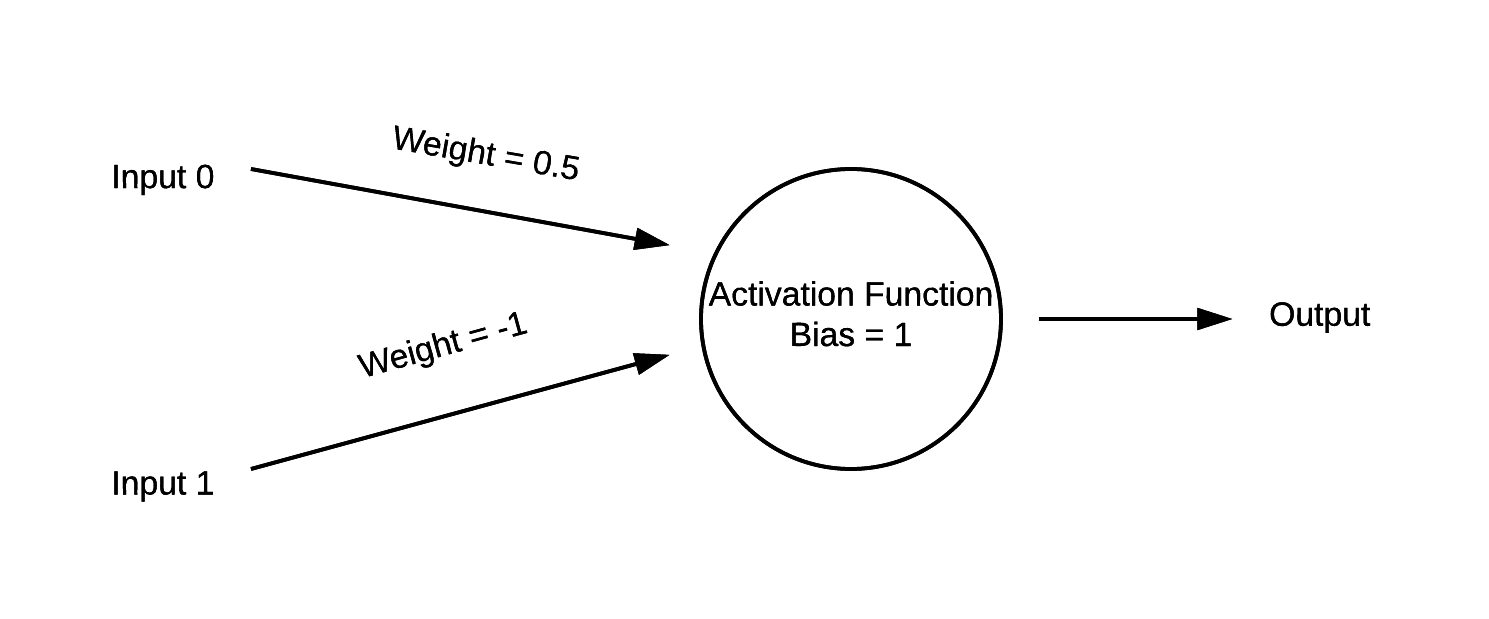
\includegraphics{Perceptron}
     \caption{Perceptron}
     \label{fig:perceptron}
\end{figure}

The Perceptron Training Rule is how weights are selected to produce the correct output during training.
As in \parencite{MLANN}, a common way to train a perceptron is to start with random weights and change them during training as per the training rule.
This rule follows the formula in Equation \ref{eqn:perceptron1}, where xi is the input and Equation \ref{eqn:perceptron2} is valid:
\begin{equation}\label{eqn:perceptron1}
    w_{i} \leftarrow w_{i} + \Delta w_{i}
\end{equation}

\begin{equation}\label{eqn:perceptron2}
    \Delta w_{i} = n(t-o)x_{i}
\end{equation}

In Equation \ref{eqn:perceptron2}, "t is the target output for the current training example, o is the output generated by the perceptron, and n is the positive constant called the learning rate" \parencite{MLANN}.
The output of a neuron is calculated using the activation function.
This Perceptron Training Rule assumes that there are two sets of instances, a
positive and negative set (class x and - in Figure \ref{fig:ls}), and that they are linearly separable, as in demonstrated in Figure \ref{fig:ls}. 

\begin{figure}[h]
	\centering
    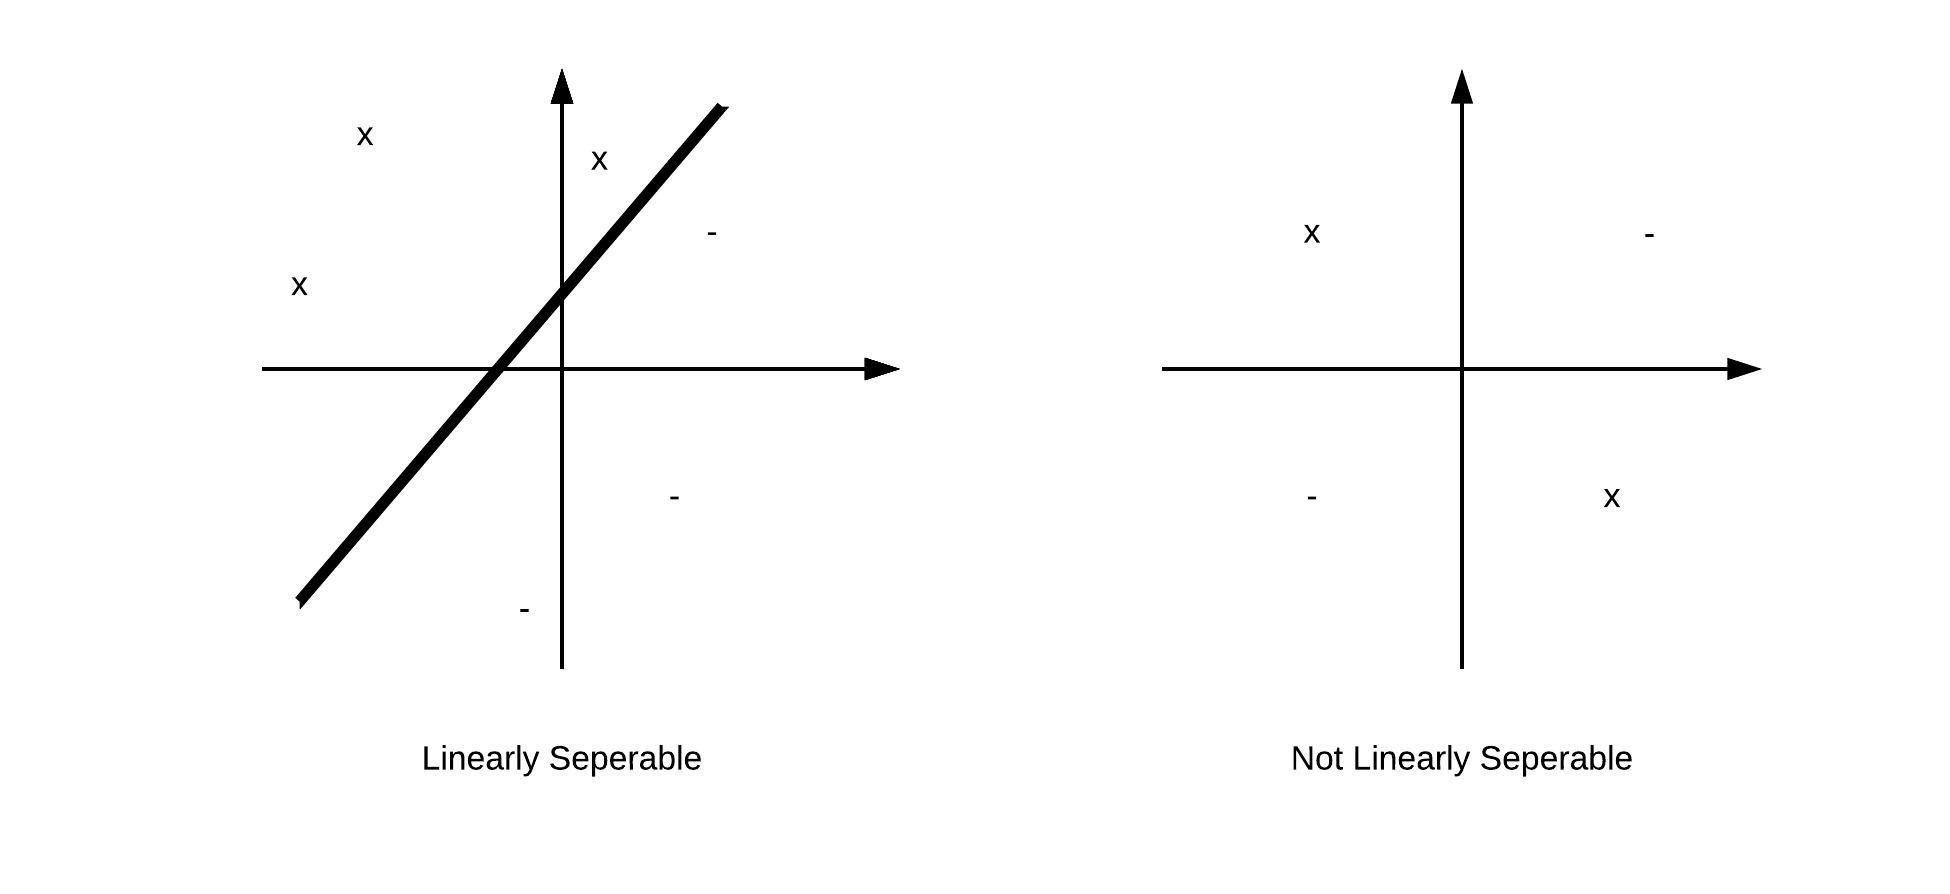
\includegraphics{LS}
     \caption{Linearly Separable, adapted from \parencite{MLANN}}
     \label{fig:ls}
\end{figure}

A perceptron is trained using supervised learning. When the perceptron
classifies a result, it is told if it is correct or not. If the result is
incorrect, weights are changed in value so that this error can be reduced
\parencite{AI}. 

There is one major problem with perceptron learning and that is, it can't solve
a problem if there is not a clear linear separation between the classes. There
is a way in which we can attempt to solve this, through the delta rule. The
delta rule utilises gradient descent to find the best weight for the training
samples \parencite{MLANN}. We will discuss gradient descent in the next section.

\tocless\subsubsection{Multi Layered Perceptron}
Multi-Layer Perceptrons (MLPs) are made up of multiple layers of perceptrons connected
together and are used to combat non-linearly separable classes.
While the delta rule can solve problems of non-linearity when there are two classes, MLPs can solve non-linearity when there are more than two classes.
Firstly, we have an input layer, followed by one or more hidden layers and then
finally an output layer.
Any ANN with more than three hidden layers is categorised as a deep neural network.

\begin{figure}[h]
	\centering
    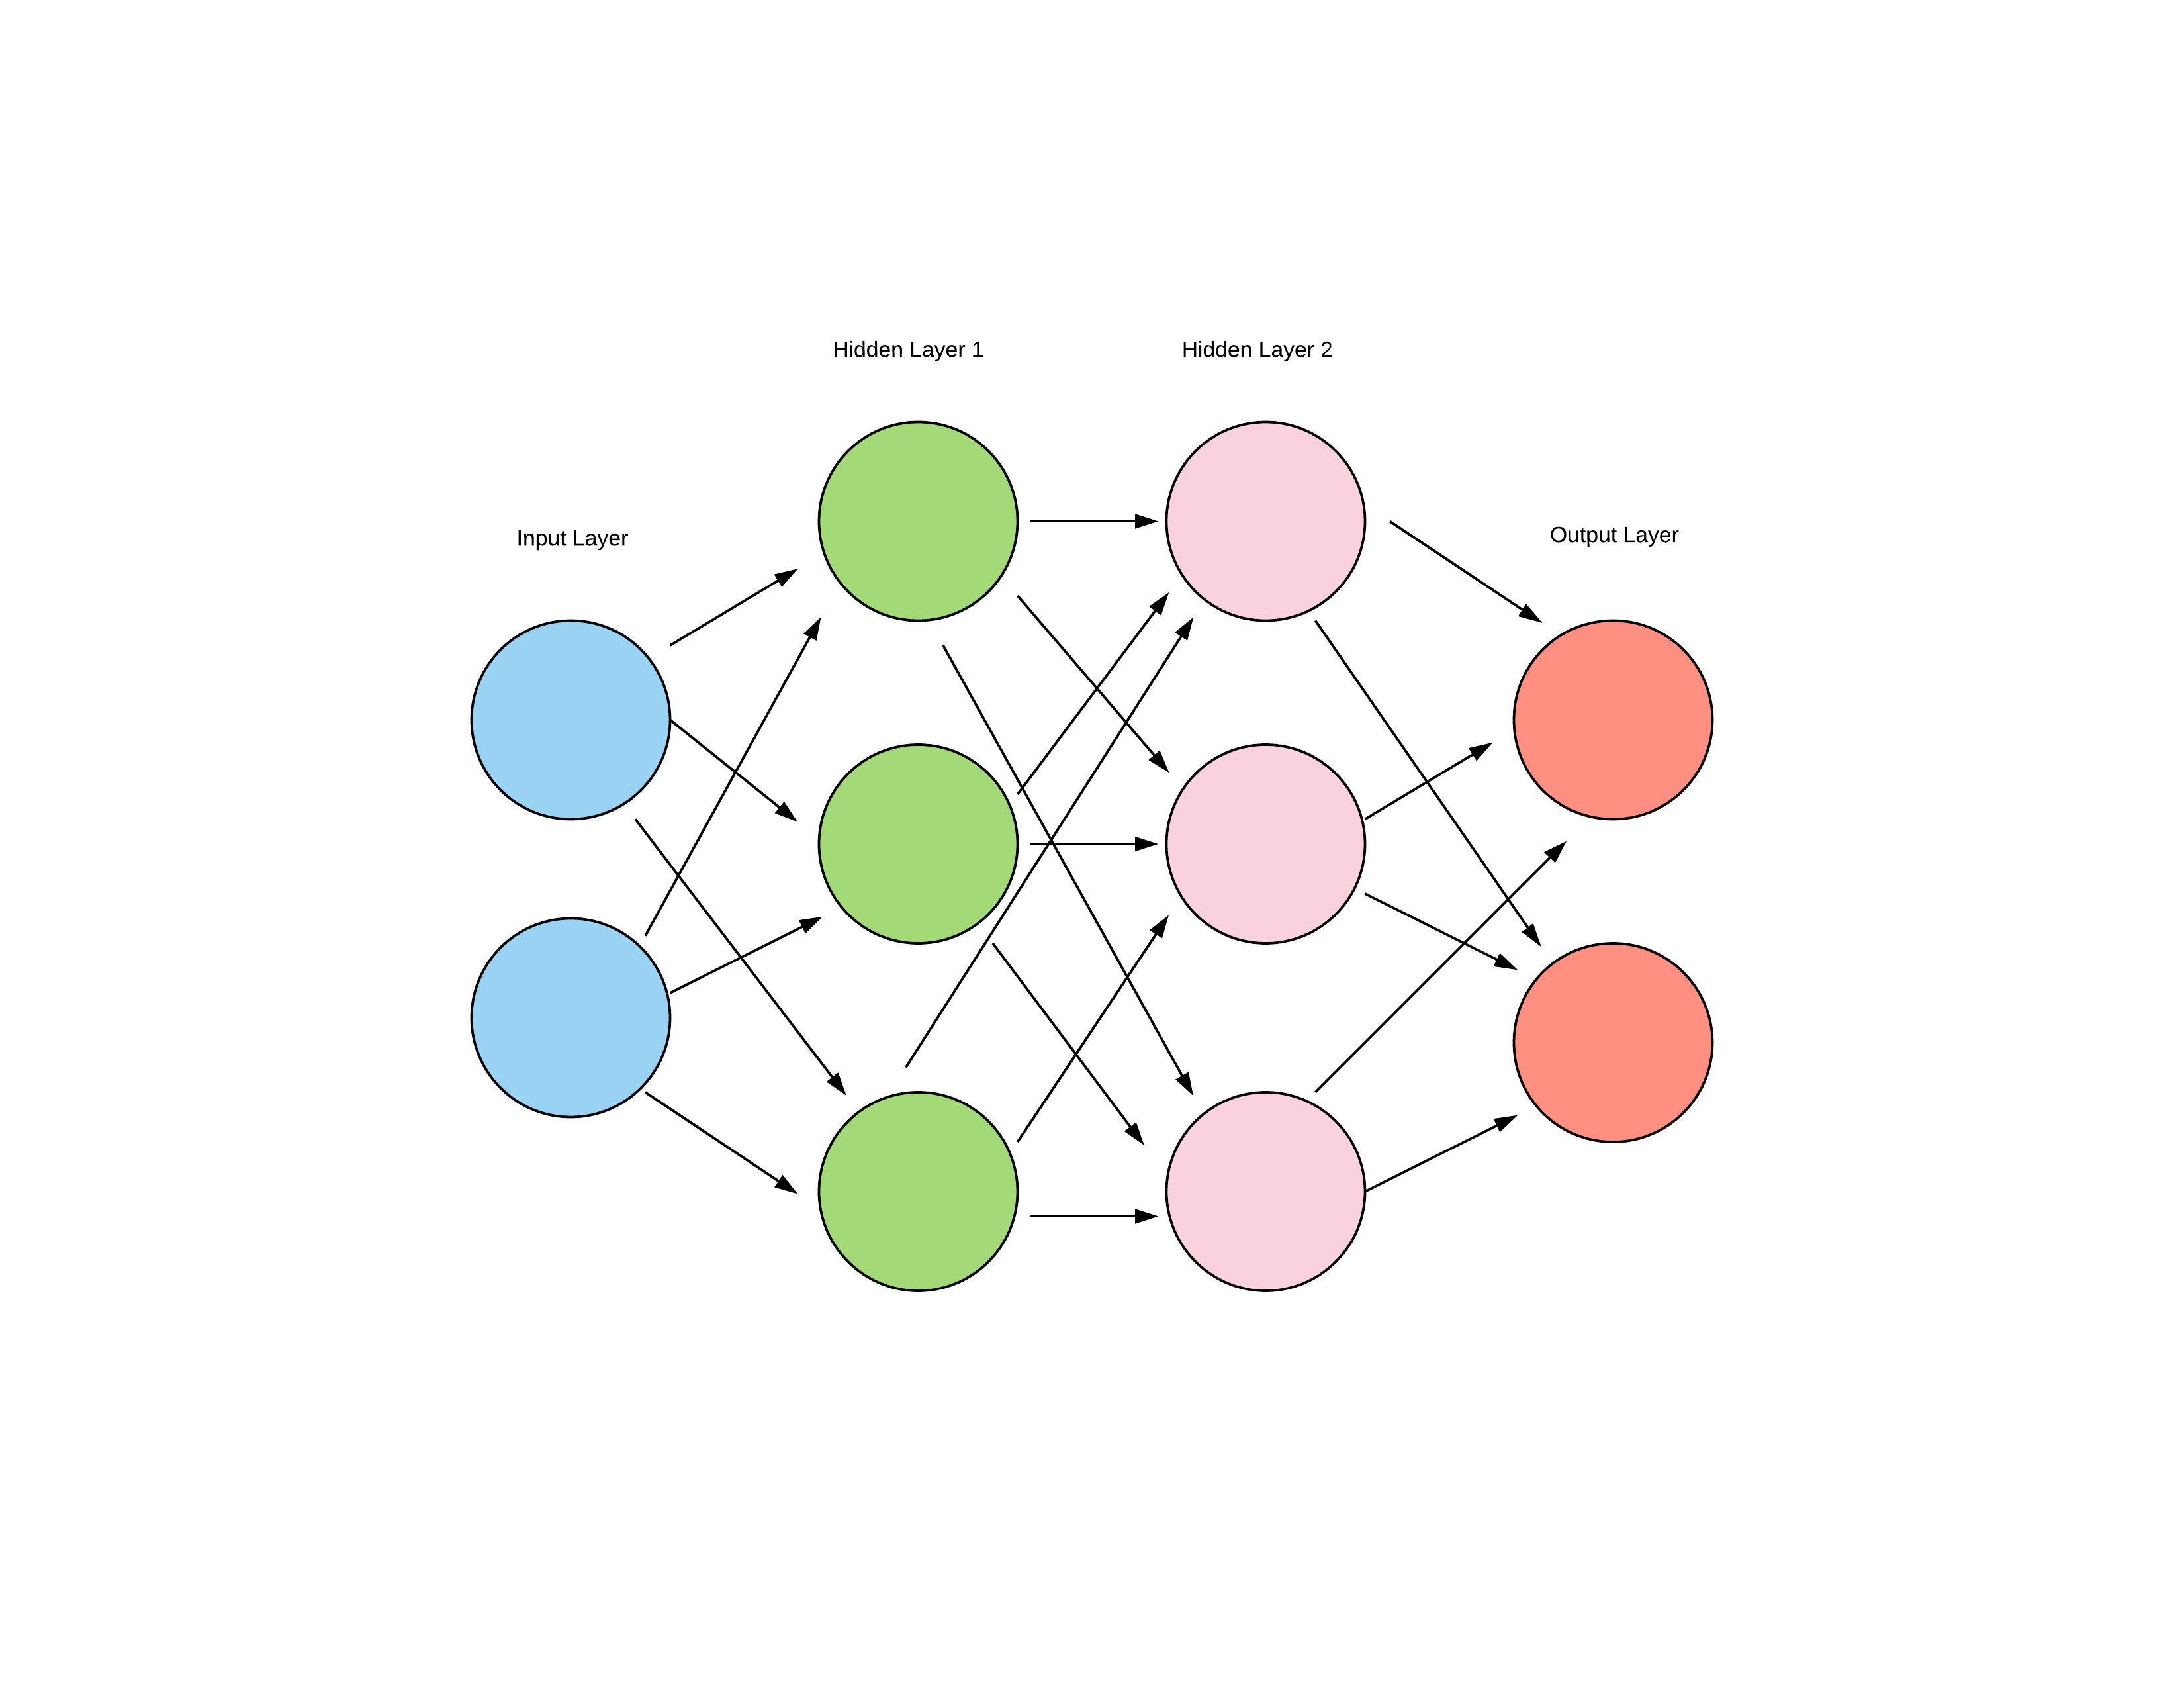
\includegraphics[width=150mm,scale=0.5]{mlp}
    \caption{Multi Layer Perceptron}
    \label{fig:mlp}
\end{figure}

The input layer of a network consists of the data that is fed into the network to be classified. The input layer passes this data to a hidden layer
whose purpose is to transform this data into something that the output layer can
understand. This transformation results in a linearly separable space that can be classified. The output layer normally consists of a class prediction.

MLPs are a class of feed forward ANNs.
These means that the output of each perceptron feeds into an input in the next
layer of the network, example seen in Figure \ref{fig:mlp}.

During training, using backpropagation for each step, the output of every neuron is calculated in each layer and then passed to the next layer. Then the error of the output is calculated, and the network calculates how each neuron in the last hidden layer effected the error. This is continued back through all the layers until the input layer \parencite{handsOnML}. The weights are then altered to try and reduce this error.

There is one large problem with MLP's and as a result CNNs were created. If one is attempting to classify images with a MLP then
each pixel in that image would have to be a separate input. This creates a
massive number of neurons through all the layers and this isn't feasible. CNN's
solve this problem which we will discuss later.



\tocless\subsubsection{Gradient Descent and backpropagation}
Gradient descent is an algorithm used to find the optimal weights to produce the
smallest prediction error. It is used to overcome problems of non-linearly
separable classes. Gradient descent search selects a random weight value and
then modifies it gradually to minimize the error. "At each step, the weight
vector is altered in the direction that produces the steepest descent along the
surface" \parencite{MLANN}. This step is iterated until the lowest value is met.

There is an error function used for the perceptron which finds the lowest error for that neuron, but it can't be used here because, since we have many neurons, there could be an error in multiple neurons.
Gradient descent is mathematically based on the derivative of a function.
The gradient of a function can be calculated by differentiating it.
As the weights are what is being controlled, "they are what we differentiate in respect to" \parencite{MLAlgorithm}.
The negative gradient of this function is followed to find the lowest possible point, hence the name gradient descent \parencite{MLAlgorithm}.

One problem with gradient descent is that if we look at Figure \ref{fig:GD}, we may
never get to the optimal point, point B. This is because we will find point A
without too many problems but when the weights change we will get too high a
slope of error and therefore will never reach point B.

Another variation of gradient descent is Stochastic Gradient Descent (SGD). SGD
is different because it updates "weights incrementally, following the
calculation of the error of each individual example" \parencite{MLANN}. 

\begin{figure}[h]
      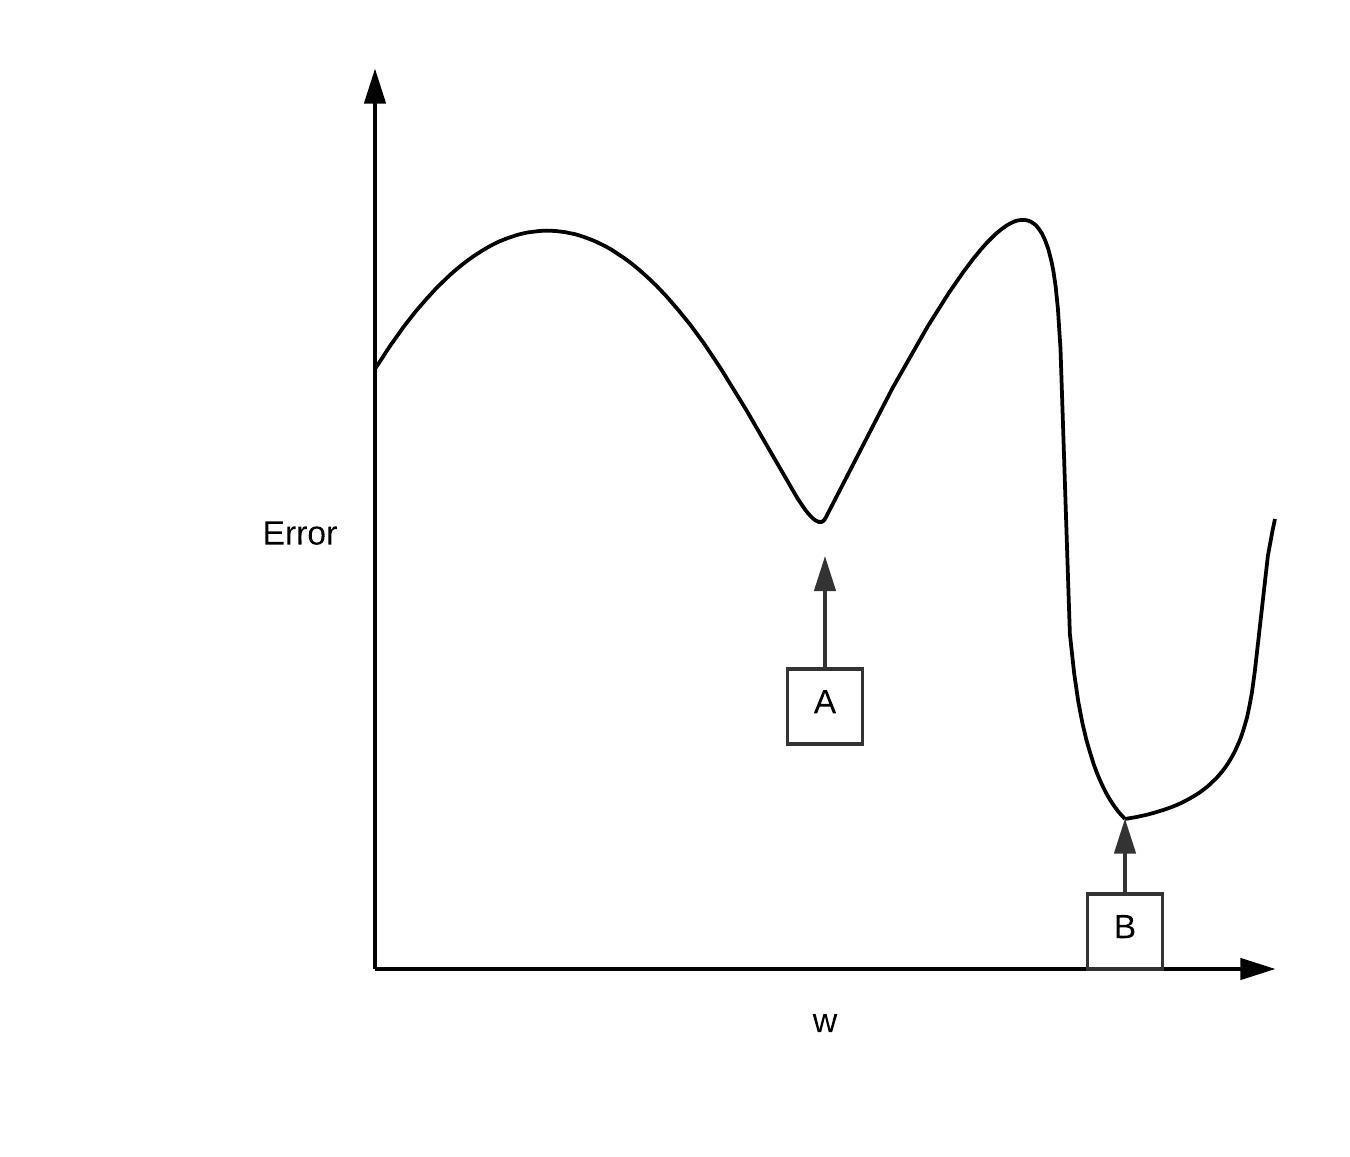
\includegraphics{GradientDescent}
      \caption{Gradient Descent}
      \label{fig:GD}
 \end{figure}

"The Backpropagation algorithm learns the weights of a multilayer network,
given a network with a fixed set of units and interconnections" \parencite{MLANN}.
Backpropagation attempts to minimize the mean squared error between the target
output and the actual output of a network.

Backpropagation works by starting at the output layer of the network and going
back through previous hidden layers, updating weights as it goes i.e. it propagates back through the network, updating the weights to try and reduce the error.

\parencite{MLANN} defined a walkthrough of the backpropagation algorithm.
For every value of Equation \ref{eqn:bp1}, in the training set where x is a vector of inputs and t is a vector of output values to act as a target:
\begin{itemize}
	\item{Run x through the network and output Equation \ref{eqn:bp2}.}
	\item{For each output k, calculate the error by Equation \ref{eqn:bp3}.}
	\item{For every hidden unit, calculate the error by Equation \ref{eqn:bp4}.}
	\item{Update weights by Equation \ref{eqn:bp5} where Equation \ref{eqn:bp5} is true.}
\end{itemize}

\begin{equation}\label{eqn:bp1}
    \vec{x}, \vec{t}
\end{equation}

\begin{equation}\label{eqn:bp2}
    o_{u}
\end{equation}

\begin{equation}\label{eqn:bp3}
    \delta_{k} \leftarrow o_{k}(1 - o_{k})(t_{k} - o_{k}) 
\end{equation}

\begin{equation}\label{eqn:bp4}
    \delta_{h} \leftarrow o_{h}(1 - o_{h}) \sum_{k \in outputs}   w_{kh}\delta_{k}
\end{equation}

\begin{equation}\label{eqn:bp5}
    w_{ji} \leftarrow w_{ji} + \Delta w_{ji}
\end{equation}

\begin{equation}\label{eqn:bp6}
    \Delta w_{ji} = \delta_{j} x_{ji}
\end{equation}


\section{Convolutional Neural Networks Overview}
Convolutional Neural Networks (CNN's) are essentially a Multi Layered Percetron with a
special structure. CNN's have one major difference from a MLP, they have extra
layer of convolution and pooling. The architecture of a convolution network can
be seen in Figure \ref{fig:convNet}.

\begin{figure}
	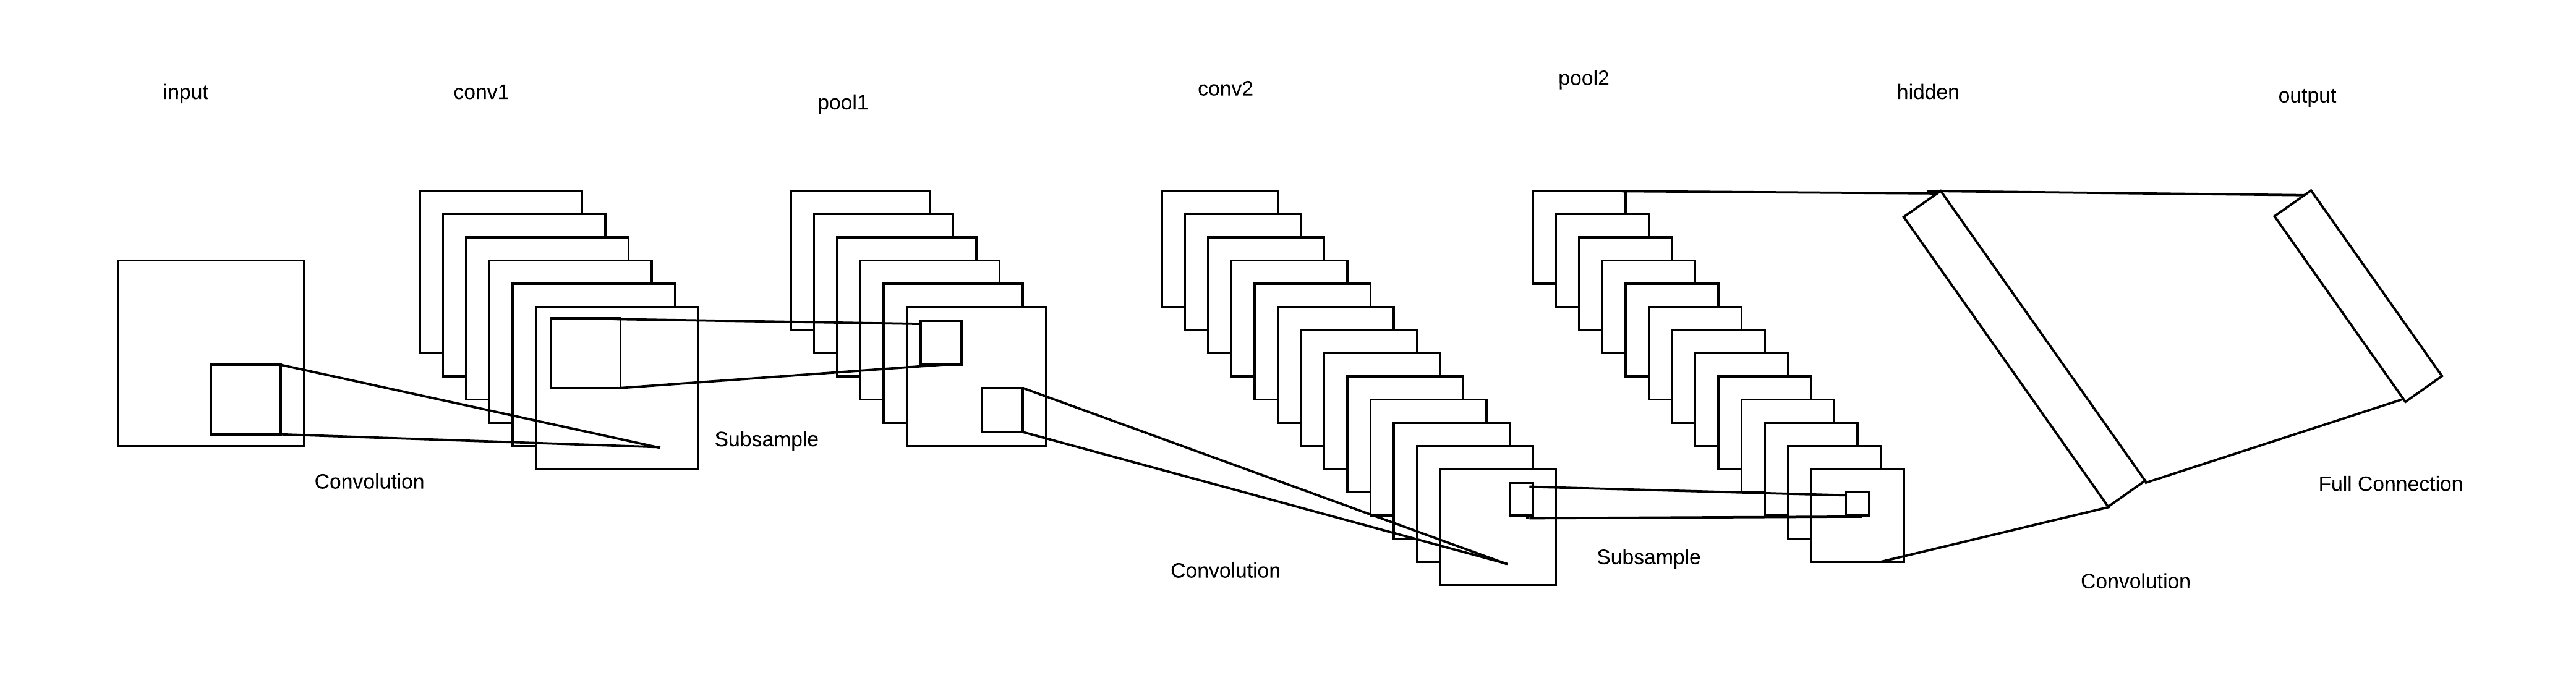
\includegraphics[width=150mm, scale=0.5]{convNet}
	\caption{CNN Architecture}
	\label{fig:convNet}
\end{figure}

Figure \ref{fig:XtoRec} show an image that we want to compare against
Figure \ref{fig:XtoComp}.
For humans, it is quite easy to determine that these images are very similar but
for a computer this task is surprisingly difficult.

So what a CNN does, to combat this problem, is to take a small feature from
Figure \ref{fig:XtoRec} and compare it to a subsection of Figure \ref{fig:XtoComp}.
The CNN multiplies the feature and a section of Figure \ref{fig:XtoComp}, adds
up the results and divides by 9. This then gives a decimal value of how likely
it is that the feature is in the part of the image, as seen in Figure
\ref{fig:convoluted}.
This is called filtering. The Convolutional layer is composed of carrying out
this filtering for every single possible location in Figure \ref{fig:XtoComp}.
\begin{figure}
	\caption{Image filtering}
    \label{fig:filter}
      \begin{subfigure}[b]{0.4\textwidth}
          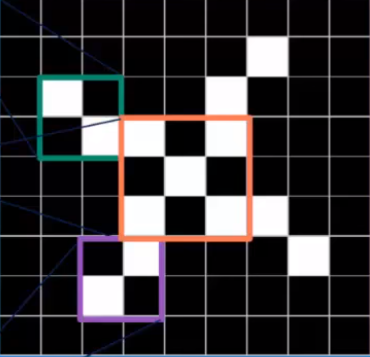
\includegraphics[width=\textwidth]{XtoRec}
          \caption{Image to Classify}
          \label{fig:XtoRec}
      \end{subfigure}
    %
      \begin{subfigure}[b]{0.4\textwidth}
      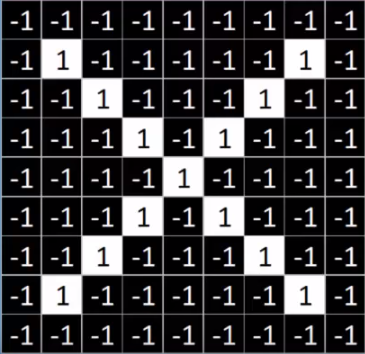
\includegraphics[width=\textwidth]{XtoComp}
      \caption{Image to Compare}
      \label{fig:XtoComp}
      \end{subfigure}
\end{figure}

\begin{figure}
    \caption{Image Convolution}  
    \begin{subfigure}[b]{0.4\textwidth}
          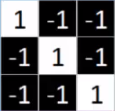
\includegraphics[width=\textwidth]{ImageFeature}
          \caption{Image Feature to Search}
          \label{fig:feature}
      \end{subfigure}
     %
      \begin{subfigure}[b]{0.4\textwidth}
           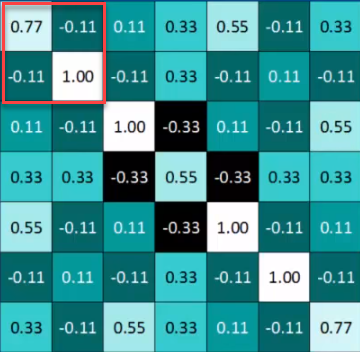
\includegraphics[width=\textwidth]{ConvImage}x
           \caption{Convoluted Image}
           \label{fig:convoluted}
      \end{subfigure}
\end{figure}
\begin{figure}
    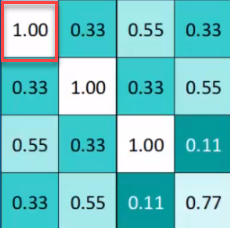
\includegraphics[width=50mm,scale=0.5]{PooledImage}
    \caption{Pooled Image}
    \label{fig:pooled}
\end{figure}
Next is the Pooling Layer, what this layer does, is it takes the convoluted
layer output, you can use Figure \ref{fig:convoluted} as reference, and from a
user defined size ie. 2x2, gets either the highest decimal value (Max pooling)
or the average value (Mean pooling) and records that as the new value for the
section. This is then applied to the entire image. As we can see in Figure
\ref{fig:pooled} we know have a much smaller image stack in which to classify,
thus making the computation easier.

In between the Convolution and Pooling layer, there is sometimes a Normalization
layer. This Normalization layer creates Rectified Linear Units (RLU's). In other
words, if we take Figure \ref{fig:convoluted}, it changes all minus values to
zero.

There are some problems with CNN's however. One of the main problems is that you
need a very large dataset in order to produce am accurate model and the training
can be very time consuming without a GPU.

\section{Convolution Neural Networks Extended}

\subsection*{Fully Convolutional Networks}
A Fully Convolutional Network is one that does not have a fully connected layer
and in a fully connected layers place is another convolution layer.

\section{Support Vector Machine}
A Support Vector Machine (SVM) is a machine learning algorithm that has been
very popular before the use of a CNN was mainstream.
Many of the texts that will be analysed later use SVMs for their classification.

A SVM works by creating an n-dimensional space, with n as the number of
inputs you have \parencite{svm}. The SVM algorithm finds the hyperplane that splits this space.
This hyperplane can then be used for classification. 
An SVM casts the problem to a higher dimensional space and this can solve a problem when the classes are not linearly separable.
This can be seen in Figure \ref{fig:svm}, where on the left there is no clear way to separate the classes but once the problem is cast to another dimensional, the separation is clear.

\begin{figure}[h]
    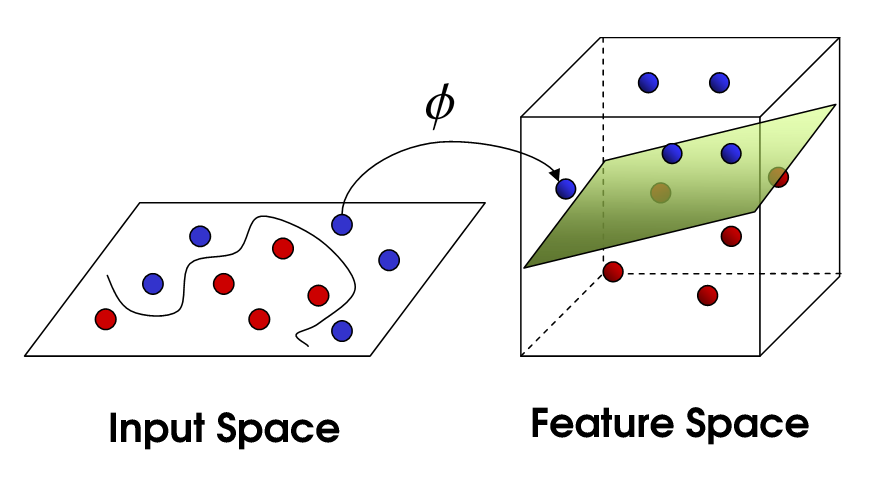
\includegraphics[scale=0.35]{svm}
    \caption{Support Vector Machine Applicability sourced from https://stackoverflow.com/questions/9480605/what-is-the-relation-between-the-number-of-support-vectors-and-training-data-and}
    \label{fig:svm}
\end{figure}

There are benefits and liabilities to using a SVM.
They can be very accurate and can work efficiently with small datasets but unfortunately it can take a large amount of time to train. 

\section{Evaluating the Output}
There are various different metrics that can be used for evaluating the output
of a classifier or segmentation algorithm, many of which we have seen in previous
sections. I was analyse a few of these evaluations of results so that I can use
them as a reference to apply to my own experiments. I will also look into some
problems associated with evaluating models.

\subsection{Research into Diagnosing Errors in Object Detectors}
There has been some research into the question of how to evaluate object
detectors, one of which I will discuss in detail \textcite{diagnosingErrors}.
This paper in question "analyzes the influences of object characteristics on
detection performance and the frequency and impact of different types of false
positives" \textcite{diagnosingErrors}. They found that there were many effects
that had influence on detectors as follows:
\begin{itemize}
    \item{occlusion}
    \item{size}
    \item{aspect ratio}
    \item{visibility of parts}
    \item{viewpoint}
    \item{localization error}
    \item{confusion with semantically similar objects}
    \item{confusion with other labeled objects}
    \item{confusion with background}
\end{itemize}

The research team goes on to analyse false positives in object detectors.
Localization errors were a large factor. This is were bounding boxes overlap to
other objects in the image. Confusion with similar objects had a large influence
on false positives also by which, for example, a dog detector had a high score
for a cat \textcite{diagnosingErrors}. Confusion with dissimilar objects and
confusion with background are the categories of the rest of the false positives
they measured.

In conclusion the team would that "Most false positives are due to misaligned
detection windows or confusion with similar objects"
\textcite{diagnosingErrors}. They had some recommendations towards improves
detectors as follows:
\begin{itemize}
	\item{Smaller objects are less likely to be detected}
	\item{Localization could be improved}
	\item{Reduce confusion with similar categories}
	\item{Robustness to object variation}
	\item{More detailed analysis}
\subsection{Detection Average Precision}
See \ref{fig:dap}.
\begin{figure}
	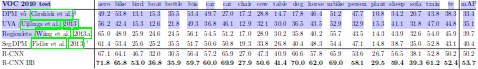
\includegraphics[width=150mm,scale=0.5]{DAP}
	\caption{Detection Average Precision \textcite{donahue}}
    \label{fig:dap}
\end{figure}

\subsection{Mean Average Precision}
See \ref{fig:MAP}.
		\begin{figure}
			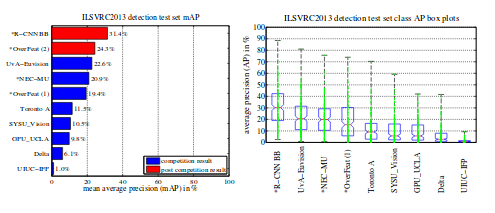
\includegraphics[width=150mm,scale=0.5]{MAP}
			\caption{Mean Average Precision \textcite{donahue}}
			\label{fig:MAP}
		\end{figure}
		
\subsection{Distribution of top-ranked false positives}
See \ref{fig:DFP}.
		\begin{figure}
			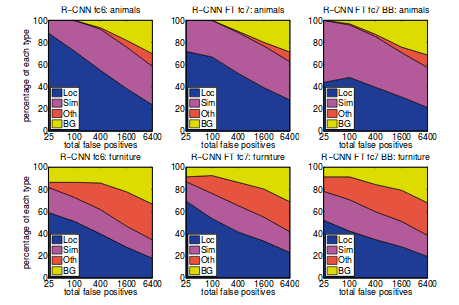
\includegraphics[width=150mm,scale=0.5]{DFP}
			\caption{Distribution of top-ranked false positives \textcite{donahue}}
			\label{fig:DFP}
		\end{figure}
		

\subsection{Segmentation Mean Accuracy}
See \ref{fig:SMP}.
		\begin{figure}
			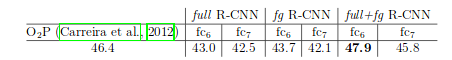
\includegraphics[width=150mm,scale=0.5]{SMP}
			\caption{Segmentation Mean Accuracy \textcite{donahue}}
			\label{fig:SMP}
		\end{figure}
		

\subsection{Per-category segmentation accuracy}
See \ref{fig:PCATSA}.
		\begin{figure}
			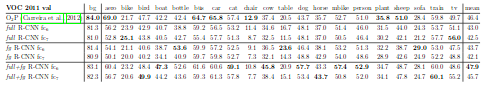
\includegraphics[width=150mm,scale=0.5]{PCATSA}
			\caption{Per-category segmentation accuracy \textcite{donahue}}
			\label{fig:PCATSA}
		\end{figure}
		

\subsection{Per-class segmentation accuracy}
\See \ref{fig:PCLASSA}.
		\begin{figure}
			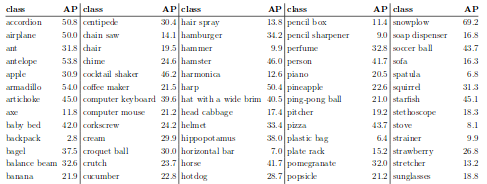
\includegraphics[width=150mm,scale=0.5]{PCLASSSA}
			\caption{Per-class segmentation accuracy \textcite{donahue}}
			\label{fig:PCLASSA}
		\end{figure}
		



\section{Dietary Assessment using Computer Vision}
\subsection{Convolution Neural Networks}
Many researchers have used convolutional neural networks for image
classification with various network architectures and many have used a food image dataset.
Some of these papers will be looked at below.
A summary of their results can be seen in Table \ref{cnn_summary}.

\parencite{deepLearning} focused on a deep learning approach to food image recognition based
their neural network architecture on Inception-ResNet and Inception V3.
Deep learning is a term usually given to algorithms based on neural networks.
They also used the Food-101 dataset. For this system, Google's
Tensorflow was used for image preprocessing. Preprocessing was needed as the
environmental background is different in many food images. Because of these
"Grey World method and Histogram equalization" \parencite{deepLearning} were
used.
Amazon Web Services (AWS) Graphics Processing Units (GPU) instances were used for training.
AWS instances are cloud servers.
The results on completion were quite impressive with a Top-1 Accuracy of 72.55\% and a Top-5 Accuracy of 91.31\%.

Another research team in Japan, \parencite{yanaiFood} researched this topic. This was built off previous research they had carried out in the field \parencite{kawano2014food}.
They were aware of how
difficult the problem was and therefore employed many techniques to solve the
problem such as "pre-training with the large-scale ImageNet data, fine-tuning
and activation features extracted from the pre-trained DCNN". 
In conclusion, they found that the "fine-tuned DCNN which was pre-trained
with 2000 categories" from ImageNet was the best method. A
DCNN is a Deep Convolution Neural Network. 
A network can become a DCNN when the number of hidden layers is larger than three.
While many of the CNNs discussed have been DCNN, most are just labeled as CNNs.
The achieved results of 78.77\% for Top-1 Accuracy in the UECFOOD100 dataset.


\parencite{kagayaFood} also employed the use of convolutional neural networks for
image detection. They used a CNN for the "tasks of food detection and recognition
through parameter optimization".
They found that a CNN is much better suited to the task than a Support Vector
Machine (SVM). They achieved an overall classification accuracy of 93.8\%
against their baseline accuracy of 89.7\%. This accuracy
was calculated using a dataset that they created specifically for this task.
When they had completed the task they analysed the trained convolutional kernels
and came to an interesting conclusion. They found that "color features are
essential to food image recognition".


The last paper that will be analysed, \parencite{deepFood}, oriented around using a Convolutional Neural
Network for food image recognition, focuses on developing a dietary assessment
application for use on a smart phone. They used the UEC-256 and Food-101 dataset
for their experiments and achieved impressive results.
They used a Convolutional Neural Network but "with a few major optimizations,
such as optimized model and an optimized convolution technique". 
They used the Inception module for their CNN. After the
inception module was complete, they made the GoogleNet architecture by combining modules. In
total, the network had 22 layers.
They achieved the results shown in Table \ref{resultsDeepFood}.

\begin{table}[h]
	\centering
	\caption{DeepFood Results}
	\label{resultsDeepFood}
	\begin{tabular}{lll}
		& Top-1  & Top-5  \\
		UEC-256                   & 54.7\% & 81.5\% \\
		UEC-100                   & 76.3\% & 94.6\% \\
		Food-101                  & 77.4\% & 93.7\% \\
		UEC-256 With Bounding Box & 63.8\% & 87.2\% \\
		  UEC-100 With Bounding Box & 77.2\% & 94.8\%
	\end{tabular}
\end{table}

\parencite{nutrinet} developed a new neural architecture specifically for detecting food and drink images using deep convolutional neural networks called NutriNet.
The trained network was to be used to aid patients with Parkinson's disease in monitoring their diet.
NutriNet was created based off of the AlexNet architecture.
The dataset used for this study consisted of approximately 500 images for each of over 500 classes.
Through this dataset a Top-1 accuracy of 86.72\& and a Top-5 accuracy of 94.47\% was recorded.
A smart phone application was used for real world testing which brought a Top-5 accuracy of 55\%.
The application also saved these real world images from the smart phone to increase their dataset size.
In conclusion, the team found that there were modifications that could be made to the NutriNet architecture as real world images didn't perform incredibly well due to occlusion and background noise in the images.
The detection and recognition steps were separated in this architecture.
The team also acknowledges that joining these steps into a single DCNN may be successful and should be explored.

\begin{table}[h]
	\centering
	\caption{Summary of results in CNN based methods}
	\label{cnn_summary}
	\begin{tabular}{lll}
		Title                                & Dataset     & Top-1 Accuracy \\
		\parencite{deepLearning} 			 & Food 101    & 72.55\%  \\
		\parencite{yanaiFood}               	 & UECFood101  & 78.77\%  \\
		\parencite{kagayaFood}       		 & Own dataset & 93.80\%   \\
		\parencite{deepFood}                  & Food 101    & 77.40\%  	\\
		\parencite{nutrinet}                  & Own dataset & 86.72\%
	\end{tabular}
\end{table}



\subsection{Support Vector Machines}
While Convolutional Neural Networks have proven very successful in recent years, there are many other methods of food image identification and classification that have been employed by food image recognition researchers, such as SVMs.
A summary of the results of these methods can be seen in Table \ref{other_dietary_summary}.

In a study conducted by \parencite{kernelLearning}, a practical use for food image recognition in the form of a mobile phone application was proposed.
In order to classify the images, multiple kernel learning(MKL) was used.
MKL is similar to a SVM expect that instead of a single kernel during training, MKL " treats with a combined kernel which is a weighted linear combination of several single kernels" \parencite{kernelLearning}.
The idea behind this is that different food types are distinguishable by different factors and using this method, the best of these factors can be used for classification of that food type.
In the experiments carried out, three different factors were used for learning:
\begin{itemize}
	\item{Colour Histograms}
	\item{Gabor Texture Features}
	\item{Bag-of-Features using Scale Invariant Feature Transformation (SIFT)}
\end{itemize}

According to \parencite{sift}, "SIFT features are formed by computing the gradient at each pixel" in a window and then using the correct level of the Gaussian filters where the window was detected.
50 different classifiers were created in a SVM using MKL with " one category as a positive set and other 49 categories as a negative set" \parencite{kernelLearning}.
For each of these categories, a web scrape was carried out and then the best 100 images for each scrape was manually selected. Five-fold cross validation was utilised in the paper.

MKL proceeded to yield results of 61.34\% on the 50 food types and a Top-3 accuracy of 80.05\%.
The prototype mobile phone application resulted in a 37.55\% user accuracy.
While the Top 1 and Top 5 accuracies for this model show promising results, the user accuracy is very poor.
This would suggest that the classifier does not work well with real life images and is possibly overfitting to the training and testing dataset.
MKL classifiers may not be promising for generalisation.

Another quite successful study was carried out using a SVM.
\parencite{novelSVM} had established that both colour and texture are very important, but they also decided that shape and size are vital features to analyse.
The proposed system has two main parts, segmentation followed by classification.
To create a 'robust' system, a 'Robust Handling of Different Lighting Conditions' module is added to the system \parencite{novelSVM}.
This is so that various lighting conditions don't cause colour data to be distorted. 

Since this paper calls for calorie estimation, the first step of the system calculates the size of the food portion. In order to do this, a coin or the users thumb is included in the image taken so that the pixel count of the thumb and the food can be compared to estimate the size. Following this the image is segmented into various portions. The following step classifies each segment of the image by extracting colour, texture and shape features and inputting these into a SVM.

12 different food types were trained for this SVM with an average classification accuracy of 92.6\%.
\parencite{novelSVM} came to the conclusion that it would be difficult to use their algorithm with real data and no evidence of real-world testing was recorded.
This is unfortunate as it is difficult to get an idea of the success of the system.
Unfortunately, only 12 food types were trained and no evidence is given of how the classifier scales to more classes.

Another study that employed both a SVM and an emphasis on colour, texture and shape features, was carried out by \parencite{pouladzadeh2014measuring}.
Size was also a factor in the calorie measurement module of the system. It was found that using all four of these features increases the overall accuracy.

In order to segment the image successfully, Gabor filters were applied to separate texture features while colour was also utilised. For each segment established, size, shape, colour and texture features were extracted and using a SVM, a classification was made. The SVM used the radial basis function kernel.
Calorie estimation was also a large part of this paper, and the users thumb was taken with the food to calculate food size.

In the prototype application, once the classification had been made, the user can confirm or change the prediction. Another feature of the application was in regards to " Partially Eaten Food" \parencite{pouladzadeh2014measuring}. This was accomplished by taking a picture before and after consumption and as a result only calculated the size of the food eaten and therefore more accurate calorie counts can be produced.

15 food types were trained using the SVM with 3,000 images. The accuracy for the classifier averaged at 90.41\% using 10-fold cross-validation.
There was also a calorie count accuracy of 86\%. The best classification results were on single foods followed by non-mixed and finally mixed foods produced the worst results.

Even though \parencite{pouladzadeh2014measuring} segmented the image before classification, they still had poor results on mixed foods.
The low number of classes the classifier was trained on makes it difficult to see how effective the classifier is.
It would also be beneficial to know how long classification took on a new image as the classifier used features of colour, texture, size and shape which would be quite time consuming.

\parencite{zhu2011segmentation} had a strong focus on the segmentation aspect of a dietary assessment system.
The segmentation of the food images was achieved " using Normalized Cuts based on intensity and colour" \parencite{zhu2011segmentation}.
Normalized Cuts is a graph-based segmentation method.
To aid the segmentation aspect of this study, a common background colour was introduced to the images.
Segmentation refinement was also an important module in the experiment.
This is the process by which neighbouring segments with  the same classification label are merged together.
This also helps calculate a more accurate size estimation.
The classification of the segmented image was processed by using a SVM calculating colour and texture features.
Gabor filters were used for the texture feature extraction.

In the experimental results for this study, it was found that segmentation was not always successful " when the region of interest is camouflaged by making its boundary faint" \parencite{zhu2011segmentation}. In their case, it was a can of coke that wasn't segmented correctly.
The classification accuracy was of 56.2\% and 95.5\% with ground truth segmentation data.
19 classes of food were used in this study with approximately 60 images per class.
Very little information was given in this paper on the classifier used.
The low classification results do not yield promising results for this method.

% % \tocless\subsubsection{Promising Approaches of Computer-supported Dietary Assessment and Management: 
% % Current Research Status and Available Applications}
% % \parencite{arens2015promising}

% \tocless\subsubsection{Novel Technologies for Assessing Dietary Intake: Evaluating the
% Usability of a Mobile Telephone Food Record Among Adults and Adolescents}
% \parencite{novelTech}

There was a study carried out on food identification through a smart phone application by \parencite{chen2012automatic}.
This study resulted in an application that allows a user to send an image of their food to a server which can give them an automatic response in 12 seconds.
This back-end service can have 34 threads working concurrently as stated at the time the paper was published.

A SVM is used to classify the image across 50 categories trained on around 100 images each.
The SVM uses SIFT and Local Binary pattern feature extractors.
A separate SVM was trained for each of these extractors and was merged together using a " Multi-class AdaBoost algorithm" \parencite{chen2012automatic}.

The study produced a top-1 accuracy  of 68.3\%. Accuracy of 80.6\%, 84.8\% and 90.9\% were recorded using top-2, top-3 and top-5 accuracy respectively.
Unfortunately, real-world image classifcation results were not recorded from the smartphone applications.
Due to this, it is difficult to measure the efficacy of the classifier, even more so because they only had 50 classes.  

% % \tocless\subsubsection{An Overview of the Technology Assisted Dietary Assessment Project at Purdue University}
% % \parencite{khanna2010overview}

\parencite{villalobos2012image} researched the question of using a computer vision approach to this topic. They focus mostly on the segmentation and region of interest calculation of the system in their study.

The system in question requires two images of the food, one from above and one from the side. This helps with size estimation. The users thumb is required to be in the image for accurate size estimation. The application also requires an image after consumption as to not calculate calories for uneaten food.
The system segments the image and then extracts colour, size and shape information from each segment. This data is then used by a SVM for classification along with a nutritional database for calorie information. 
Multiple segmentation methods were tested such as:
\begin{itemize}
	\item{Semi-automatic contour definition}
	\item{Watershed transformation}
	\item{Colour rasterization}
	\item{Edge accentication}
\end{itemize}
The first two were dismissed due to poor results but the second two were used in conjunction for the segmentation aspect of the system.
\parencite{villalobos2012image} did not provide extension information on the classifier used in this study and would be therfore very difficult to replicate.
However, impressive segmentation results were obtained.

An application called "Snap-n-Eat" was proposed by \parencite{snap}.
When an image is taken using this application, the system finds saliency regions to remove the background of the image.
If the image has multiple food types present, hierarchical segmentation takes place before proceeding to a SVM. Similar segments are merged together.
These are found by using colour, texture and size.

SIFT and Histogram of Oriented Gradients (HOG) feature extractors are used on the image and these features are used by the SVM for classification.
The SVM is trained using Scholastic Gradient Descent.
\parencite{snap} also uses a Bog of Visual Words model along with k-means clustering.
An accuracy of 85\% on 15 classes was recorded using this method.

\begin{table}[]
\centering
\caption{Summary of accuracy in dietary assessment methods}
\label{other_dietary_summary}
\begin{tabular}{|p{9cm}|l|l|}
\hline
\textbf{Title}                                                         & \textbf{Classes} & \textbf{Accuracy}   \\ \hline
Food Image Recognition with Multiple Kernel Learning          & 50             & 61.3\%    \\ \hline
A Novel SVM Based Food Recognition Method                     & 12             & 92.6\%     \\ \hline
Measuring Calorie and Nutrition from Food Image               & 15             & 90.4\%    \\ \hline
Segmentation Assisted Food Classification                     & 19            & 56.2\%     \\ \hline
Large Scale Leaning for Food Image Classification             & 11             & 78.0\%       \\ \hline
Toward Dietary Assessment via Mobile Phone Video Camera       & 20             & 92.0\% \\ \hline
Automatic Chinese Food Identification and Quantity Estimation & 50             & 68.3\%     \\ \hline
Food Recognition and Nutrition Estimation on a Smartphone      & 15             & 85.0\% \\ \hline      
\end{tabular}
\end{table}

\subsection{Other Methods}
Methods outside of CNNs and SVMs are outlined below.
A summary of the results can be seen in Table \ref{other_dietary_summary} along with SVM method results.

\subsubsection*{Large Scale Learning for Food Image Classification}
\parencite{LSL_2015} proposed a food image recognition system using a Bag of Features model.
This study used over 5000 images separated into 11 classes.

A clustering algorithm was employed on this study before classification.
For the classification step, experiments were carried out using different methods:
\begin{itemize}
	\item{SVM}
	\item{ANN}
	\item{Random Forests}
\end{itemize}

The final accuracy of the system was 78\% \parencite{LSL_2015}.

% % \subsubsection*{Promising Approaches of Computer-supported Dietary Assessment and Management: 
% % Current Research Status and Available Applications}
% % \parencite{arens2015promising}

\subsubsection*{A Personal Assistive System for Nutrient Intake Monitoring}
Similar to other approaches seen thus far, \parencite{personalAssistive} employs the use of the users thumb in the image for size estimation.

Once a photo has been taken by the user with their thumb present, the system segments the food on the plate using shape, colour and texture detectors.
The system then classifies the food type based on these features.

In this paper, it was decided to allow the users to change the prediction by the system.
The thumb of each user is calibrated upon first use of the application so that size estimation can be as accurate a possible \parencite{personalAssistive}.

\subsubsection*{Toward Dietary Assessment via Mobile Phone Video Camera}
Another study into using computer vision for dietary assessment was carried out by \parencite{chen2010toward}. They had a unique medium for the topic by using a video of the dishes in question and extracting frames from these videos to get the food from different angles.

\parencite{chen2010toward} then formed a region of interest in the image, where there were the most food items and extracted colour and image features.
These image features were extracted using Maximally Stable Extremal Regions (MSER), Speeded Up Robust Features (SURF) and Star detector.

This research team also uses k-means clustering to build a bag-of-words model \parencite{chen2010toward}.

The system had results as seen below across 20 categories using five images out of each video taken of the food:
\begin{itemize}
	\item{MSER - 95\%}
	\item{SURF - 90\%}
	\item{STAR - 90\%}
\end{itemize}

% \subsubsection*{Novel Technologies for Assessing Dietary Intake: Evaluating the
% Usability of a Mobile Telephone Food Record Among Adults and Adolescents}
% \parencite{novelTech}


% % \subsubsection*{An Overview of the Technology Assisted Dietary Assessment Project at Purdue University}
% % \parencite{khanna2010overview}

\subsubsection*{Merging dietary assessment with the adolescent lifestyle}
\parencite{schap2014merging} proposed a system used by smart phones which sends an image of a users food to a back end system for computation.

Once this has been completed, the image is segmented, features are extracted from each segment and these segments are classified.
Colour and texture features are used for classification.
The user has the ability to confirm or amend predictions of the food type.

Size estimation is also an important aspect of this system.
In contrast to previous studies, \parencite{snap} uses food type shape and then those shape's geometric properties to estimate size.

This study produced results of 94\% out of 32 test cases.










\section{Object Detection Using CNNs}
Due to the issues with composite images (images with multiple items) in food image recognition, an object detection approach may prove to be successful.
If the objects (different food items) in an image could be classified seperately then the overall effiency of a nutrional assessment system, aided by deep learning, could be improved.
Ross Girshik and other contributors had some very positive results in the area
of object detection using region based convolutional neural networks. There were
four iterations of papers based on this work by Ross and groups in UC Berkley,
Microsoft and Facebook. A PHD student at the time of Ross's first paper also
completed his dissertation on the subject. These papers, their
results (Table \ref{rcnnResults}) and the changes made through each iteration will be analysed thoroughly in the proceeding sections.

In the first paper written by Ross Girshik, while researching at UC Berkeley,
focused on two main insights. These were that " one can apply high-capacity convolutional neural networks (CNNs) to bottom-up region proposals in order to localize and segment objects" and that
"when training data is scarce, supervised pre-training for n auxiliary task,
followed by domain-specific fine-tuning, yields a significant performance boost"
\parencite{rcnn}.

The system that they developed followed these steps:
\begin{itemize}
    \item{Take image as input}
    \item{Extract approximately 2000 region proposals from the image}
    \item{Compute fixed length vectors of features for the regions using a convolutional
        neural network}
    \item{Use a Support Vector Machine (SVM) to classify these regions}
    \item{Bounding box regression for final region proposals}
\end{itemize}

This system utilised selective search to gather these region proposals, but they
mention that a sliding-window detector is also an option. Ross Girshik and his
team used the open source Caffe CNN library for this system. The system is quite
efficient and scalable. It is scalable because of the fixed length vector of
features which will remain constant regardless of inputs and additional outputs.
The team evaluated their results on a few metrics and test sets as seen in Table
\ref{rcnnResults}. Explanation of the datasets used can be seen in Table \ref{datasets}.

Ross Girshik's next iteration of work on region based convolution neural
networks took place in Microsoft Research. This paper was titled "Fast R-CNN" as
its aim was to decrease training and testing time "while also increasing
detection accuracy" \parencite{fastRcnn}.

This paper analyses why RCNN \parencite{rcnn} was slow and therefore how it could be improved.
RCNN was classified to be slow because of three main factors:
\begin{itemize}
	\item{There are multiple stages to training as both a CNN and a SVM need to
		be trained.}
	\item{In training of the SVM, each region proposal must be written to disk
		and is therefore expensive.}
	\item{Object detection takes 47 seconds per image}
\end{itemize}

Due to these problems with RCNN, a new algorithm, titled Fast RCNN was proposed.
The architecture is as follows. An image is taken as input along with a
proposal for regions. The image is pushed through convolutional and pooling
layers (using max pooling). A fixed-length vector of features is then extracted
from each region proposal. These vectors are inputted to fully connected
layers for bounding box location prediction.
At detection time, a pass through of the net is all that is needed so this
runtime is significantly less than RCNN.

Due to the success of RCNN and Fast RCNN, Faster RCNN was introduced to combat
the problem of region proposal computation \parencite{fasterRcnn}.
The architecture for this system comprises of two modules. These consist of a
convolutional neural network for region proposals (RPN) which the feeds into a Fast
RCNN detector. These combine to produce a single neural network for object
detection.

Instead of training these networks separately, the team had to look at how to
share layers between the two networks. There were three options available:
\begin{itemize}
    \item{Alternating training whereby RPN is trained, and then used to train
        Fast RCNN. The Fast RCNN network is then used to initialise RPN and the
		process is iterated \parencite{fasterRcnn}. This paper follows this approach.}
    \item{Approximate joint training.}
    \item{Non- approximate joint training.}
\end{itemize}

\begin{table}[h]
    \centering
    \caption{Results from Region Based CNN Research}
    \label{rcnnResults}
    \begin{tabular}{|p{1.5cm}|l|l|l|l|l|l|}
    \hline
                    & \textbf{VOC07} & \textbf{VOC10} & \textbf{VOC11} & \textbf{VOC12} & \textbf{COCO15} &
                    \textbf{COCO16} \\ \hline
                    RCNN        & 58.5\%  & 53.7\%  & 47.9\%  & N/A     & N/A
                    & N/A      \\ \hline
                    Fast RCNN   & 70.0\%  & 68.8\%  & N/A     & 68.4\%  & N/A
                    & N/A      \\ \hline
                    Faster RCNN & 78.8\%  & N/A     & N/A     & 75.9\%  & 42.7\%
                    & N/A      \\ \hline
                    Mask RCNN   & N/A     & N/A     & N/A     & N/A     & N/A
                    & 63.1\%  \\ \hline
    \end{tabular}
\end{table}

\begin{table}[h]
\centering
\caption{Datasets}
\label{datasets}
\begin{tabular}{|p{1.65cm}|p{10.5cm}|}
\hline
\textbf{Table} & \textbf{Explanation}                                                                                                                                                                                               \\ \hline
VOC07          & The PASCAL VOC dataset is used for the PASCAL (Pattern Analysis, Statistical Modelling and Computational Learning) Visual Object Classes Challenge. \parencite{pascal-voc-2007} was used for the 2007 challenge. \\ \hline
VOC10          & The PASCAL VOC 2010 dataset was used for the 2010 challenge \parencite{pascal-voc-2010}.                                                                                                                         \\ \hline
VOC11          & The PASCAL VOC 2011 dataset was used for the 2011 challenge \parencite{pascal-voc-2011}.                                                                                                                        \\ \hline
VOC12          & The PASCAL VOC 2012 dataset was used for the 2012 challenge \parencite{pascal-voc-2012}.                                                                                                                        \\ \hline
COCO15         & The COCO (Common Objects in Context) dataset created by Microsoft (\parencite{coco}) is used to measure the efficacy of object detection algorithms. The COCO 2015 dataset was released in 2015 for training.    \\ \hline
COCO16         & An updated version of the COCO dataset was released in 2015.                                                                                                                                                       \\ \hline
\end{tabular}
\end{table}

The most recent paper on this topic was also written by Ross Girshik while
working with Facebook AI Research \parencite{maskRcnn}. Mask RCNN " extends Faster
RCNN by adding a branch for predicting an object mask in parallel with the
existing branch for bounding box regression" \parencite{maskRcnn}.
Mask RCNN has two modules, like Faster RCNN, where the first module is the
Region Proposal Network. In the second module, in parallel to classification, a
binary mask is outputted for each region. Bounding box regression and
classification are done in parallel.



\section{APIs and Libraries}
\tocless\subsection{TensorFlow}
TensorFlow is a deep learning software library for various machine learning paradigms. TensorFlow will be used to create neural networks.
TensorFlow uses a data structure called a tensor which is basically an array of n dimensions.
TensorFlow has two utilisations, through a Graphics Processing Unit (GPU) and through a Central Processing Unit (CPU).
GPU computation is recommended for CNN training. 

\tocless\subsubsection{Central Processing Unit Computation}
It is quite easy to get TensorFlow up and running if you are only using a CPU to
train. TensorFlow CPU has been successfully installed on both Windows and Ubuntu, for this project.
For Windows you can download and install using the TensorFlow website and on ubuntu you can
using apt-get. Once installed, TensorFlow can be imported into any python shell
or script for use. TensorFlow can also be used in C++. There will be various
python implementations of neural networks in Chapter 3.

\tocless\subsubsection{Graphics Processing Unit Computation}
For use with a GPU, the set up for TensorFlow is a bit more complicated. Firstly
you must check that the GPU in your machine is compatible for CUDA 8.0 using the
NVIDIA website. If your GPU is compatible, you must install CUDA after signing
up as an NVIDIA developer. CUDA 8.0 is compatible with TensorFlow.
You also need to install cudnn6.
The NVIDIA website contains tutorials to install these.
Once these are installed, download and install tensorflow-gpu.
This can be imported into python similar to CPU computation.


\tocless\subsection{OpenCV}
OpenCV is an industry wide, open source library for computer vision and machine learning \parencite{opencv}.
It has over 2500 algorithms that are available for use \parencite{opencv}.
OpenCV is supported across multiple languages and platforms such as Python, C++, C, Java, Matlab, running on Windows, Android, Mac OS and Linux \parencite{opencv}.

There is not much of the library utilised in this project due to the nature of Tensorflow but some algorithms for image reading, writing and resizing were used due to the ease of use.

\begin{lstlisting}
image = cv2.imread('image.jpg')
\end{lstlisting}

\begin{lstlisting}
resized = cv2.resize(image, (299, 299))
\end{lstlisting}

\begin{lstlisting}
cv2.imwrite('imageResized.jpg', resized)
\end{lstlisting}


\tocless\subsection{NumPy}
NumPy is a package for Python that is used for scientific computing \parencite{numpy}.
In the context of this FYP, it will be used for multi-dimensional array manipulation.

\section{Public Domain Datasets}
Some public domain datasets were used in this FYP while learning TensorFlow and conducting empirical studies.
These datasets are outlined below.
\tocless\subsection{Food-101}
\parencite{food101} created the Food-101 dataset which consists of 101 different food types.
Each food type in the dataset has 1,000 images associated.
These images can be divided up into a training, test and validation set as seen fit by the user.
The Food-101 dataset is open for public use as long as it is used for research purposes and not for commericial use.
Examples from the Food-101 dataset can be seen in below.

\begin{figure}[h] 
  \label{food} 
  \begin{minipage}[b]{0.25\linewidth}
    \centering
    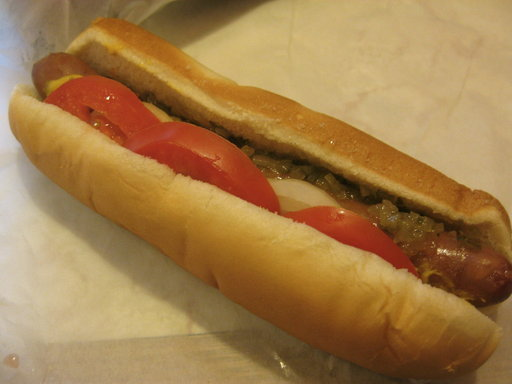
\includegraphics[width=.75\linewidth]{food1} 
    \caption{Hotdog} 
    \vspace{4ex}
  \end{minipage}%%
  \begin{minipage}[b]{0.25\linewidth}
    \centering
    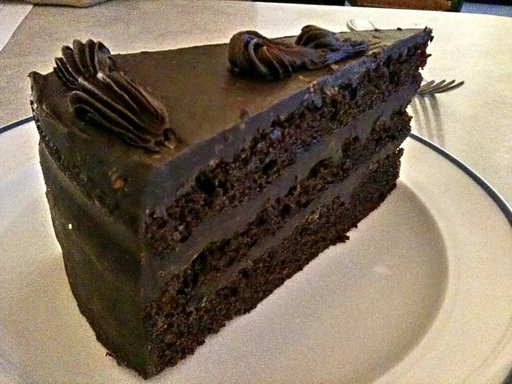
\includegraphics[width=.75\linewidth]{food2} 
    \caption{Chocolate Cake} 
  \label{fig:page2}
    \vspace{4ex}
  \end{minipage} 
  \begin{minipage}[b]{0.25\linewidth}
    \centering
    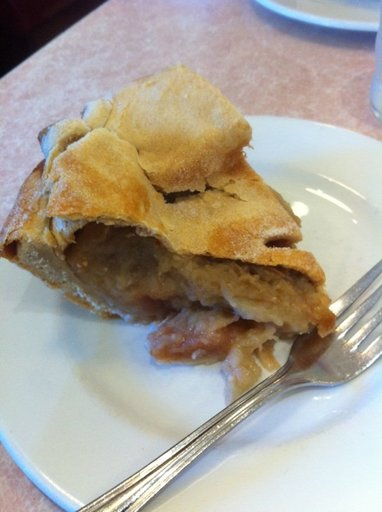
\includegraphics[width=.75\linewidth]{food3} 
    \caption{Apple Pie} 
    \vspace{4ex}
  \end{minipage}%% 
  \begin{minipage}[b]{0.25\linewidth}
    \centering
    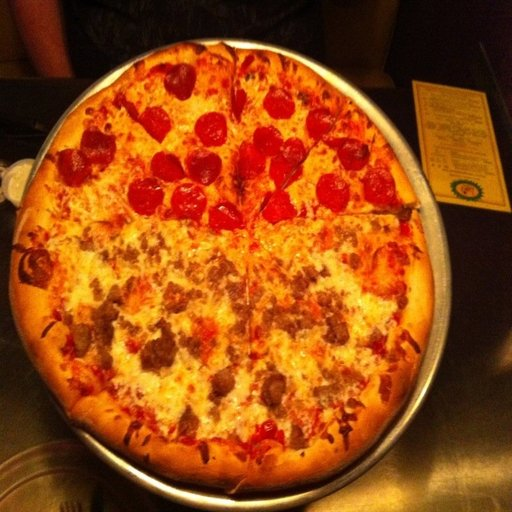
\includegraphics[width=.75\linewidth]{food4} 
    \caption{Pizza} 
    \vspace{4ex}
  \end{minipage} 
\end{figure}

\tocless\subsection{MNIST}
The MNIST dataset (created by \parencite{mnist}) consists of 70,000 hand written digits.
It is widely used in introductory CNN tutorials.
The dataset is split into 60,000 training images and 10,000 test images.
All the images are of the same dimensions.
Examples from the MNIST dataset can be seen in below.

\begin{figure}[h] 
  \label{mnistDataset} 
  \begin{minipage}[b]{0.25\linewidth}
    \centering
    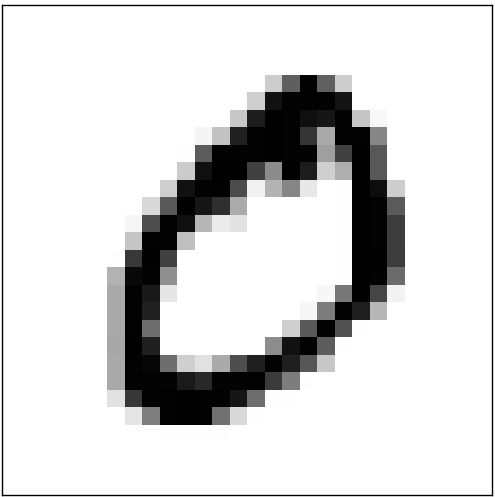
\includegraphics[width=.75\linewidth]{mnist0} 
    \caption{MNIST 0} 
    \vspace{4ex}
  \end{minipage}%%
  \begin{minipage}[b]{0.25\linewidth}
    \centering
    
\includegraphics[width=.75\linewidth]{mnist2} 
    \caption{MNIST 2} 
  \label{fig:page2}
    \vspace{4ex}
  \end{minipage} 
  \begin{minipage}[b]{0.25\linewidth}
    \centering
    
\includegraphics[width=.75\linewidth]{mnist4} 
    \caption{MNIST 4} 
    \vspace{4ex}
  \end{minipage}%% 
  \begin{minipage}[b]{0.25\linewidth}
    \centering
    
\includegraphics[width=.75\linewidth]{mnist5} 
    \caption{MNIST 5} 
    \vspace{4ex}
  \end{minipage} 
\end{figure}

\tocless\subsection{CIFAR-10}
\parencite{cifar} created the CIFAR-10 dataset which consists of 10 classes.
Each of the 10 classes has 6,000 32x32 colour image associated and these are split between a 5,000 image training set and a 1,000 image test set.
There are five training batches and one test batch in the dataset.
The test set contains 1,000 randomly selected images from each class.
The training batches consist of random orderings of the remaining images.
Examples from the CIFAR-10 dataset can be seen below.

\begin{figure}[h] 
  \label{cifar10} 
  \begin{minipage}[b]{0.25\linewidth}
    \centering
    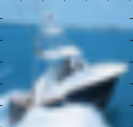
\includegraphics[width=.75\linewidth]{cifar1} 
    \caption{CIFAR-10 Truck} 
    \vspace{4ex}
  \end{minipage}%%
  \begin{minipage}[b]{0.25\linewidth}
    \centering
    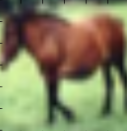
\includegraphics[width=.75\linewidth]{cifar2} 
    \caption{CIFAR-10 Horse} 
  \label{fig:page2}
    \vspace{4ex}
  \end{minipage} 
  \begin{minipage}[b]{0.25\linewidth}
    \centering
    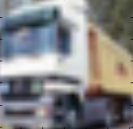
\includegraphics[width=.75\linewidth]{cifar3} 
    \caption{CIFAR-10 Boat} 
    \vspace{4ex}
  \end{minipage}%% 
  \begin{minipage}[b]{0.25\linewidth}
    \centering
    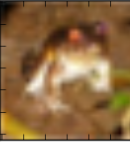
\includegraphics[width=.75\linewidth]{cifar4} 
    \caption{CIFAR-10 Frog} 
    \vspace{4ex}
  \end{minipage} 
\end{figure}

\section{Conclusion}
This chapter has covered a comprehensive survey of literature along with an overview of the underlying concepts to the approaches used in the literature.
This survey has covered the topics of using CNNs, SVMs and other methods for nutritional assessment.
Topics also covered include evaluating the output, object detection using CNNS, neural computing, an overview of CNNS and SVMS and an overview of the technologies used in this project.

From the literature review, there are many different approaches that have been promising in the area of using deep learning for nutritional assessment.
It has been decided to attempt to replicate the work carried out by \parencite{yanaiFood} with some modifications that will be outlined in the following chapters.
While this approach will be attempted, there are many viable options that can still be investigated for future work.



\chapter{Introduction to Using Tensorflow}
\section{Template for Experiments}
The template followed for all experiments in chapters three, four and five is outlined in Figure \ref{fig:expTemplate}.

\begin{table}[]
\centering
\caption{Experiment Template}
\label{fig:expTemplate}
\begin{tabular}{|p{4cm}|p{11cm}|}
Experiment Section   & Rationale                \\
Overview             & An explanation of the purpose of the experiment along with how it is carried out. \\
Network Architecture & An explanation of the network architecture used in the experiment. If the architecture has been explained in another experiment, the architecture will only be referenced by name.                       \\
Dataset              & The dataset used for the experiment, with its source and an overview of its details. A brief mention will be made in following experiments.                       \\
API's                & Reference to the technologies used as outlined in Chapter 2.                      \\
Script               & Snippets of the script used for the experiment.                       \\
Results              & The results acquired from the experiment, usually in the form of a percentage accuracy.                       \\
Empirical Analysis   & States any information gained from the experiment and speculation for the reasoning of the results.                      
\end{tabular}
\end{table}

\section{Udemy Tutorial}
\label{udemy1}
\subsection*{Overview}
There are many on line resources that are geared towards helping deep learning novices.
One of these resources is a course on Udemy titled 'Complete Guide to Tensorflow for Deep Learning with Python' \textcite{udemy}.
This course has a section on Convolutional Neural Networks which has been followed and completed.

\subsection*{Network Architecture}
The architecture for this network is very simple as it is an introductory CNN.
It consists of two convolutional layers, two max pooling layers and a fully connected layer.

\subsection*{Dataset}
This CNN is trained on the MNIST dataset.
This dataset consists of 70000 handwritten digits \textcite{mnist}.

\subsection*{API's}
This experiment was carried out in a jupyter notebook using tensorflow.

\subsection*{Script}
\begin{lstlisting}

#Helper Functions

#INIT WEIGHTS
def init_weights(shape):
    init_random_dist = tf.truncated_normal(shape, stddev = 0.1)
    return tf.Variable(init_random_dist)

#INIT BIAS
def init_bias(shape):
    init_bias_vals = tf.constant(0.1, shape = shape)
    return tf.Variable(init_bias_vals)

#CONV2D
def conv2d(x, W):
    #x -> [batch, H, W, Channels]
    #W -> [filterH, filterW, ChannelsIn, ChannelsOut]
    return tf.nn.conv2d(x, W, strides = [1,1,1,1], padding = 'SAME')

#POOLING
def max_pool_2by2(x):
    #x -> [batch, H, W, Channels]
    return tf.nn.max_pool(x, ksize = [1,2,2,1], strides = [1,2,2,1], padding = 'SAME')

    #NORMAL (FULLY CONNECTED)
def normal_full_layer(input_layer, size):
    input_size = int(input_layer.get_shape()[1])
    W = init_weights([input_size, size])
    b = init_bias([size])
return tf.matmul(input_layer, W) + b
\end{lstlisting}

\begin{lstlisting}
#32 features for every 5 x 5 patch with 1(grayscale)
convo_1 = convolutional_layer(x_image, shape = [5,5,1,32])
convo_1_pooling = max_pool_2by2(convo_1)

convo_2 = convolutional_layer(convo_1_pooling, shape = [5,5,32,64])
convo_2_pooling = max_pool_2by2(convo_2)

convo_2_flat = tf.reshape(convo_2_pooling, [-1,7*7*64])
full_layer_one = tf.nn.relu(normal_full_layer(convo_2_flat, 1024))
\end{lstlisting}

\begin{lstlisting}
with tf.Session() as sess:
    sess.run(init)
    
    for i in range(steps):
        batch_x, batch_y = mnist.train.next_batch(32)
        batch_test = mnist.test.next_batch(32)
        sess.run(train, feed_dict = {x:batch_x, y_true:batch_y, hold_prob:0.5})
        if i%500 == 0:
            print("ON STEP: {}".format(i))
            print("ACCURACY: ")
            match = tf.equal(tf.argmax(y_pred, 1), tf.argmax(y_true, 1))
            acc = tf.reduce_mean(tf.cast(match, tf.float32))
            print(sess.run(acc, feed_dict = {x:batch_test, y_true:mnist.test.labels, hold_prob:1.0}))
            print('\n')
            
    sess.run(acc, feed_dict = {x:mnist.test.images} )

#Final Accuracy 0.973
\end{lstlisting}

\subsection*{Results}
The Final Accuracy for this experiment was of 97.3\%.


\section{Udemy Tutorial 2}
\label{udemy2}
\subsection*{Objective}
Similar to the previous experiment \ref{udemy2}, this experiment is a Udemy course exercise \parencite{udemy}. In contrast, this does not use a dataset built into TensorFlow so therefore, there is extra configuration to be done on the dataset.

\subsection*{Network Architecture}
Same architecture as in \ref{udemy1}.

\subsection*{Dataset}
The CIFAR-10 dataset is used here. 
This has 60000 images split into 10 classes and a test set of 1000 images \parencite{cifar}.

\subsection*{Script}
\begin{lstlisting}[style=Python]
def unpickle(file):
    import pickle
    with open(file, 'rb') as fo:
        cifar_dict = pickle.load(fo, encoding='bytes')
    return cifar_dict

dirs = ['batches.meta','data_batch_1','data_batch_2','data_batch_3','data_batch_4','data_batch_5','test_batch']

all_data = [0,1,2,3,4,5,6]

for i,direc in zip(all_data,dirs):
    all_data[i] = unpickle(CIFAR_DIR+direc)

batch_meta = all_data[0]
data_batch1 = all_data[1]
data_batch2 = all_data[2]
data_batch3 = all_data[3]
data_batch4 = all_data[4]
data_batch5 = all_data[5]
test_batch = all_data[6]
\end{lstlisting}

\begin{lstlisting}[style=Python]
def set_up_images(self):
        
        print("Setting Up Training Images and Labels")
        
        # Vertically stacks the training images
        self.training_images = np.vstack([d[b"data"] for d in self.all_train_batches])
        train_len = len(self.training_images)
        
        # Reshapes and normalizes training images
        self.training_images = self.training_images.reshape(train_len,3,32,32).transpose(0,2,3,1)/255
        # One hot Encodes the training labels (e.g. [0,0,0,1,0,0,0,0,0,0])
        self.training_labels = one_hot_encode(np.hstack([d[b"labels"] for d in self.all_train_batches]), 10)
        
        print("Setting Up Test Images and Labels")
        
        # Vertically stacks the test images
        self.test_images = np.vstack([d[b"data"] for d in self.test_batch])
        test_len = len(self.test_images)
        
        # Reshapes and normalizes test images
        self.test_images = self.test_images.reshape(test_len,3,32,32).transpose(0,2,3,1)/255
        # One hot Encodes the test labels (e.g. [0,0,0,1,0,0,0,0,0,0])
        self.test_labels = one_hot_encode(np.hstack([d[b"labels"] for d in self.test_batch]), 10)

        
    def next_batch(self, batch_size):
        # Note that the 100 dimension in the reshape call is set by an assumed batch size of 100
        x = self.training_images[self.i:self.i+batch_size].reshape(100,32,32,3)
        y = self.training_labels[self.i:self.i+batch_size]
        self.i = (self.i + batch_size) % len(self.training_images)
return x, y
\end{lstlisting}

\begin{lstlisting}[style=Python]
cross_entropy = tf.reduce_mean(tf.nn.softmax_cross_entropy_with_logits(labels = y_true, logits = y_pred))
optimizer = tf.train.AdamOptimizer(learning_rate = 0.001)
train = optimizer.minimize(cross_entropy)
init = tf.global_variables_initializer()
with tf.Session() as sess:
    sess.run(tf.global_variables_initializer())

    for i in range(10000):
        batch = ch.next_batch(100)
        sess.run(train, feed_dict={x: batch[0], y_true: batch[1], hold_prob: 0.5})
        
        # PRINT OUT A MESSAGE EVERY 100 STEPS
        if i%1000 == 0:
            
            # Test the Train Model
            matches = tf.equal(tf.argmax(y_pred,1),tf.argmax(y_true,1))

            acc = tf.reduce_mean(tf.cast(matches,tf.float32))
            testSet = ch.next_test_batch(100)
            print('Accuracy: ')
            print(sess.run(acc,feed_dict={x:testSet[0] ,y_true:testSet[1],hold_prob:1.0}))
print('\n')
\end{lstlisting}

\subsection*{Results}
A Final Accuracy of 71\% was reached.

\subsection*{Analysis}


\section{Using the Food 101 dataset}
\label{food101}
\subsection*{Objective}
For the next experiment, it was decided to use the Food-101 dataset.
An on line tutorial was used to create a dataset in TensorFlow using image directories on disk \parencite{file_dir_code}.
Tutorials used previously were also utilized for this experiment \parencite{udemy} and \parencite{cifar}.

\subsection*{Network Architecture}
A similar network architecture to the previous two experiments (\ref{udemy1} and \ref{udemy2}) was used here.

\subsection*{Dataset}
The Food-101 dataset was used for this experiment \parencite{food101}.

\subsection*{Script}
\begin{lstlisting}[style=Python]
# Reading the dataset
# 2 modes: 'file' or 'folder'
def read_images(dataset_path, mode, batch_size):
    imagepaths, labels = list(), list()
    if mode == 'file':
        # Read dataset file
        data = open(dataset_path, 'r').read().splitlines()
        for d in data:
            imagepaths.append(d.split(' ')[0])
            labels.append(int(d.split(' ')[1]))
    elif mode == 'folder':
        # An ID will be affected to each sub-folders by alphabetical order
        label = 0
        # List the directory
        try:  # Python 2
            classes = sorted(os.walk(dataset_path).next()[1])
        except Exception:  # Python 3
            classes = sorted(os.walk(dataset_path).__next__()[1])
        # List each sub-directory (the classes)
        for c in classes:
            c_dir = os.path.join(dataset_path, c)
            try:  # Python 2
                walk = os.walk(c_dir).next()
            except Exception:  # Python 3
                walk = os.walk(c_dir).__next__()
            # Add each image to the training set
            for sample in walk[2]:
                # Only keeps jpeg images
                if sample.endswith('.jpg') or sample.endswith('.jpeg'):
                    imagepaths.append(os.path.join(c_dir, sample))
                    labels.append(label)
            label += 1
    else:
raise Exception("Unknown mode.")
\end{lstlisting}

\begin{lstlisting}[style=Python]
# Convert to Tensor
    imagepaths = tf.convert_to_tensor(imagepaths, dtype=tf.string)
    labels = tf.convert_to_tensor(labels, dtype=tf.int32)
    # Build a TF Queue, shuffle data
    image, label = tf.train.slice_input_producer([imagepaths, labels],
                                                 shuffle=True)

    # Read images from disk
    image = tf.read_file(image)
    image = tf.image.decode_jpeg(image, channels=CHANNELS)

    # Resize images to a common size
    image = tf.image.resize_images(image, [IMG_HEIGHT, IMG_WIDTH])

    # Normalize
    image = image * 1.0/127.5 - 1.0

    # Create batches
    X, Y = tf.train.batch([image, label], batch_size=batch_size,
                          capacity=batch_size * 8,
                          num_threads=4)

    return X, Y

\end{lstlisting}

\begin{lstlisting}[style=Python]
# Start training
with tf.Session() as sess:

    # Run the initializer
    sess.run(init)

    # Start the data queue
    tf.train.start_queue_runners()

    # Training cycle
    for step in range(1, num_steps+1):

        if step % display_step == 0:
            # Run optimization and calculate batch loss and accuracy
            _, loss, acc = sess.run([train_op, loss_op, accuracy])
            print("Step " + str(step) + ", Minibatch Loss= " + \
                  "{:.4f}".format(loss) + ", Training Accuracy= " + \
                  "{:.3f}".format(acc))
        else:
            # Only run the optimization op (backprop)
            sess.run(train_op)

print("Optimization Finished!")
\end{lstlisting}

\subsection*{Results}
The final accuracy for this model was 18.8\% after 5000 steps.

\subsection*{Analysis}
The poor accuracy of this model is to be expected due to the simple architecture of the network and the fact that 101 classes is a lot to process.

\chapter{Training Using the Inception-V3 Model Architecture}

\section{Retrain ImageNet Inception V3 Model}
\label{inception}
\subsection*{Objective}
For this experiment, it was decided to take inspiration from
\parencite{yanaiFood}, where pre-training was used training a model for food
classification. In order to achieve this, the final layer of the
Inception V3 model which was trained on the ImageNet dataset had to be retrained. This is called
Transfer Learning.
A tutorial, created by Google, on the TensorFlow website was followed
for direction on this process \parencite{retrainInception}.

Firstly, to retrain the final layer of a model, a dataset must be
prepared in the correct way. The Food-101 dataset \parencite{food101}
was used for this experiment, which will be analysed below.

This dataset contrasts with \parencite{yanaiFood} as they used the UECFOOD100 dataset.
The food-101 dataset was chosen due to larger number of images per class.
The UECFOOD100 dataset has 100 images per class while the food-101 dataset has 1000 images per class.
The dataset must be structured so that
there is a separated directory for each class with the directory name as the class
name. These directories should contain all the images for this class. 

Once this dataset has been set up correctly, a directory can be found on GitHub
which contains the necessary files for this tutorial. When the directory has
been downloaded, the following command can be executed:
\begin{lstlisting}[style=Command]
python tensorflow/examples/image_retraining/retrain.py \ --image_dir
~/dataset_directory
\end{lstlisting}

The first thing that the script will do is create bottleneck files for the
images. A bottleneck is a term used to define the final layer before the output
layer. This is so that for each image, we do not have to push it through the
entire network during training \parencite{retrainInception}.

After, the bottlenecks are created, the training can be completed. The images
are split into three sub directories of training, testing and validation. By
default, these images are split into percentages of 80\%, 10\% and 10\%
respectively. The model is trained at a default of 4000 steps. 

At the final stage of the script, the model is run on a batch of test images not
yet seen and a final test accuracy is displayed. This can be seen in the Script
section below.

The command used for using this model once it is trained is:
\begin{lstlisting}[style=Command]
python tensorflow/examples/label_image.py --graph=/tmp/output_graph.pb
--labels=/tmp/output_labels.txt --input_layer=Mul --output_layer=final_result
--input_mean=128 --input_std=128 --image=~/image_directory
\end{lstlisting}

\begin{table}[h]
\centering
\caption{Retrain ImageNet Inception V3 Model}
\label{my-label}
\begin{tabular}{|l|p{9cm}|}
\hline
\textbf{Network Architecture} & Inception-V3 architecture \parencite{inception}            \\ \hline
\textbf{Dataset}              & Food-101 dataset \\ \hline
\textbf{APIs and Libraries}   & TensorFlow and NumPy                                                        \\ \hline
\end{tabular}
\end{table}

\subsection*{Script}
The following snippets of code are from the retrain.py script.

\subsubsection*{Add New Layer}
\begin{lstlisting}[style=Python]
# Add new layer to the network
(train_step, cross_entropy, bottleneck_input, ground_truth_input,
final_tensor) = add_final_training_ops(
            len(image_lists.keys()), FLAGS.final_tensor_name,
            bottleneck_tensor,
            model_info['bottleneck_tensor_size'],
            model_info['quantize_layer'])
 
# Create operations to evaluate the accuracy of the model
evaluation_step, prediction = add_evaluation_step(
final_tensor, ground_truth_input)
 
# Set up weights to initial default values.
init = tf.global_variables_initializer()
sess.run(init)
\end{lstlisting}

\subsubsection*{Evaluate Model}
\begin{lstlisting}[style=Python]
# Run final test evaluation
test_bottlenecks, test_ground_truth, test_filenames = (
    get_random_cached_bottlenecks(
        sess, image_lists, FLAGS.test_batch_size, 'testing',
        FLAGS.bottleneck_dir, FLAGS.image_dir, jpeg_data_tensor,
        decoded_image_tensor, resized_image_tensor, bottleneck_tensor,
        FLAGS.architecture))
test_accuracy, predictions = sess.run(
   [evaluation_step, prediction],
   feed_dict={bottleneck_input: test_bottlenecks,
        ground_truth_input: test_ground_truth})
tf.logging.info('Final test accuracy = %.1f%% (N=%d)' %
                (test_accuracy * 100, len(test_bottlenecks)))
\end{lstlisting}

\subsection*{Results}
The final test Top-1 accuracy for this retrained model was 54.8\%.
For example, an image of pizza Figure \ref{fig:pizza}, was fed into the model with the following results:
\begin{itemize}
    \item{pizza 0.925}
    \item{pancakes 0.008}
    \item{nachos 0.007}
    \item{beef carpaccio 0.006}
    \item{tiramisu 0.004}
\end{itemize}
In contrast, Figure \ref{fig:pizza_unclassified} was not classified as a pizza.

\begin{figure}[h] 
\centering
  \label{pizzas} 
  \begin{minipage}[h]{0.5\linewidth}
    \centering
    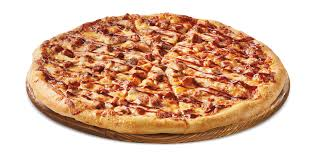
\includegraphics[scale=0.5]{pizza} 
    \caption{Pizza - sourced from https://www.cicis.com/} 
  \label{fig:pizza}
    \vspace{4ex}
  \end{minipage}%%
  \begin{minipage}[h]{0.5\linewidth}
    \centering
    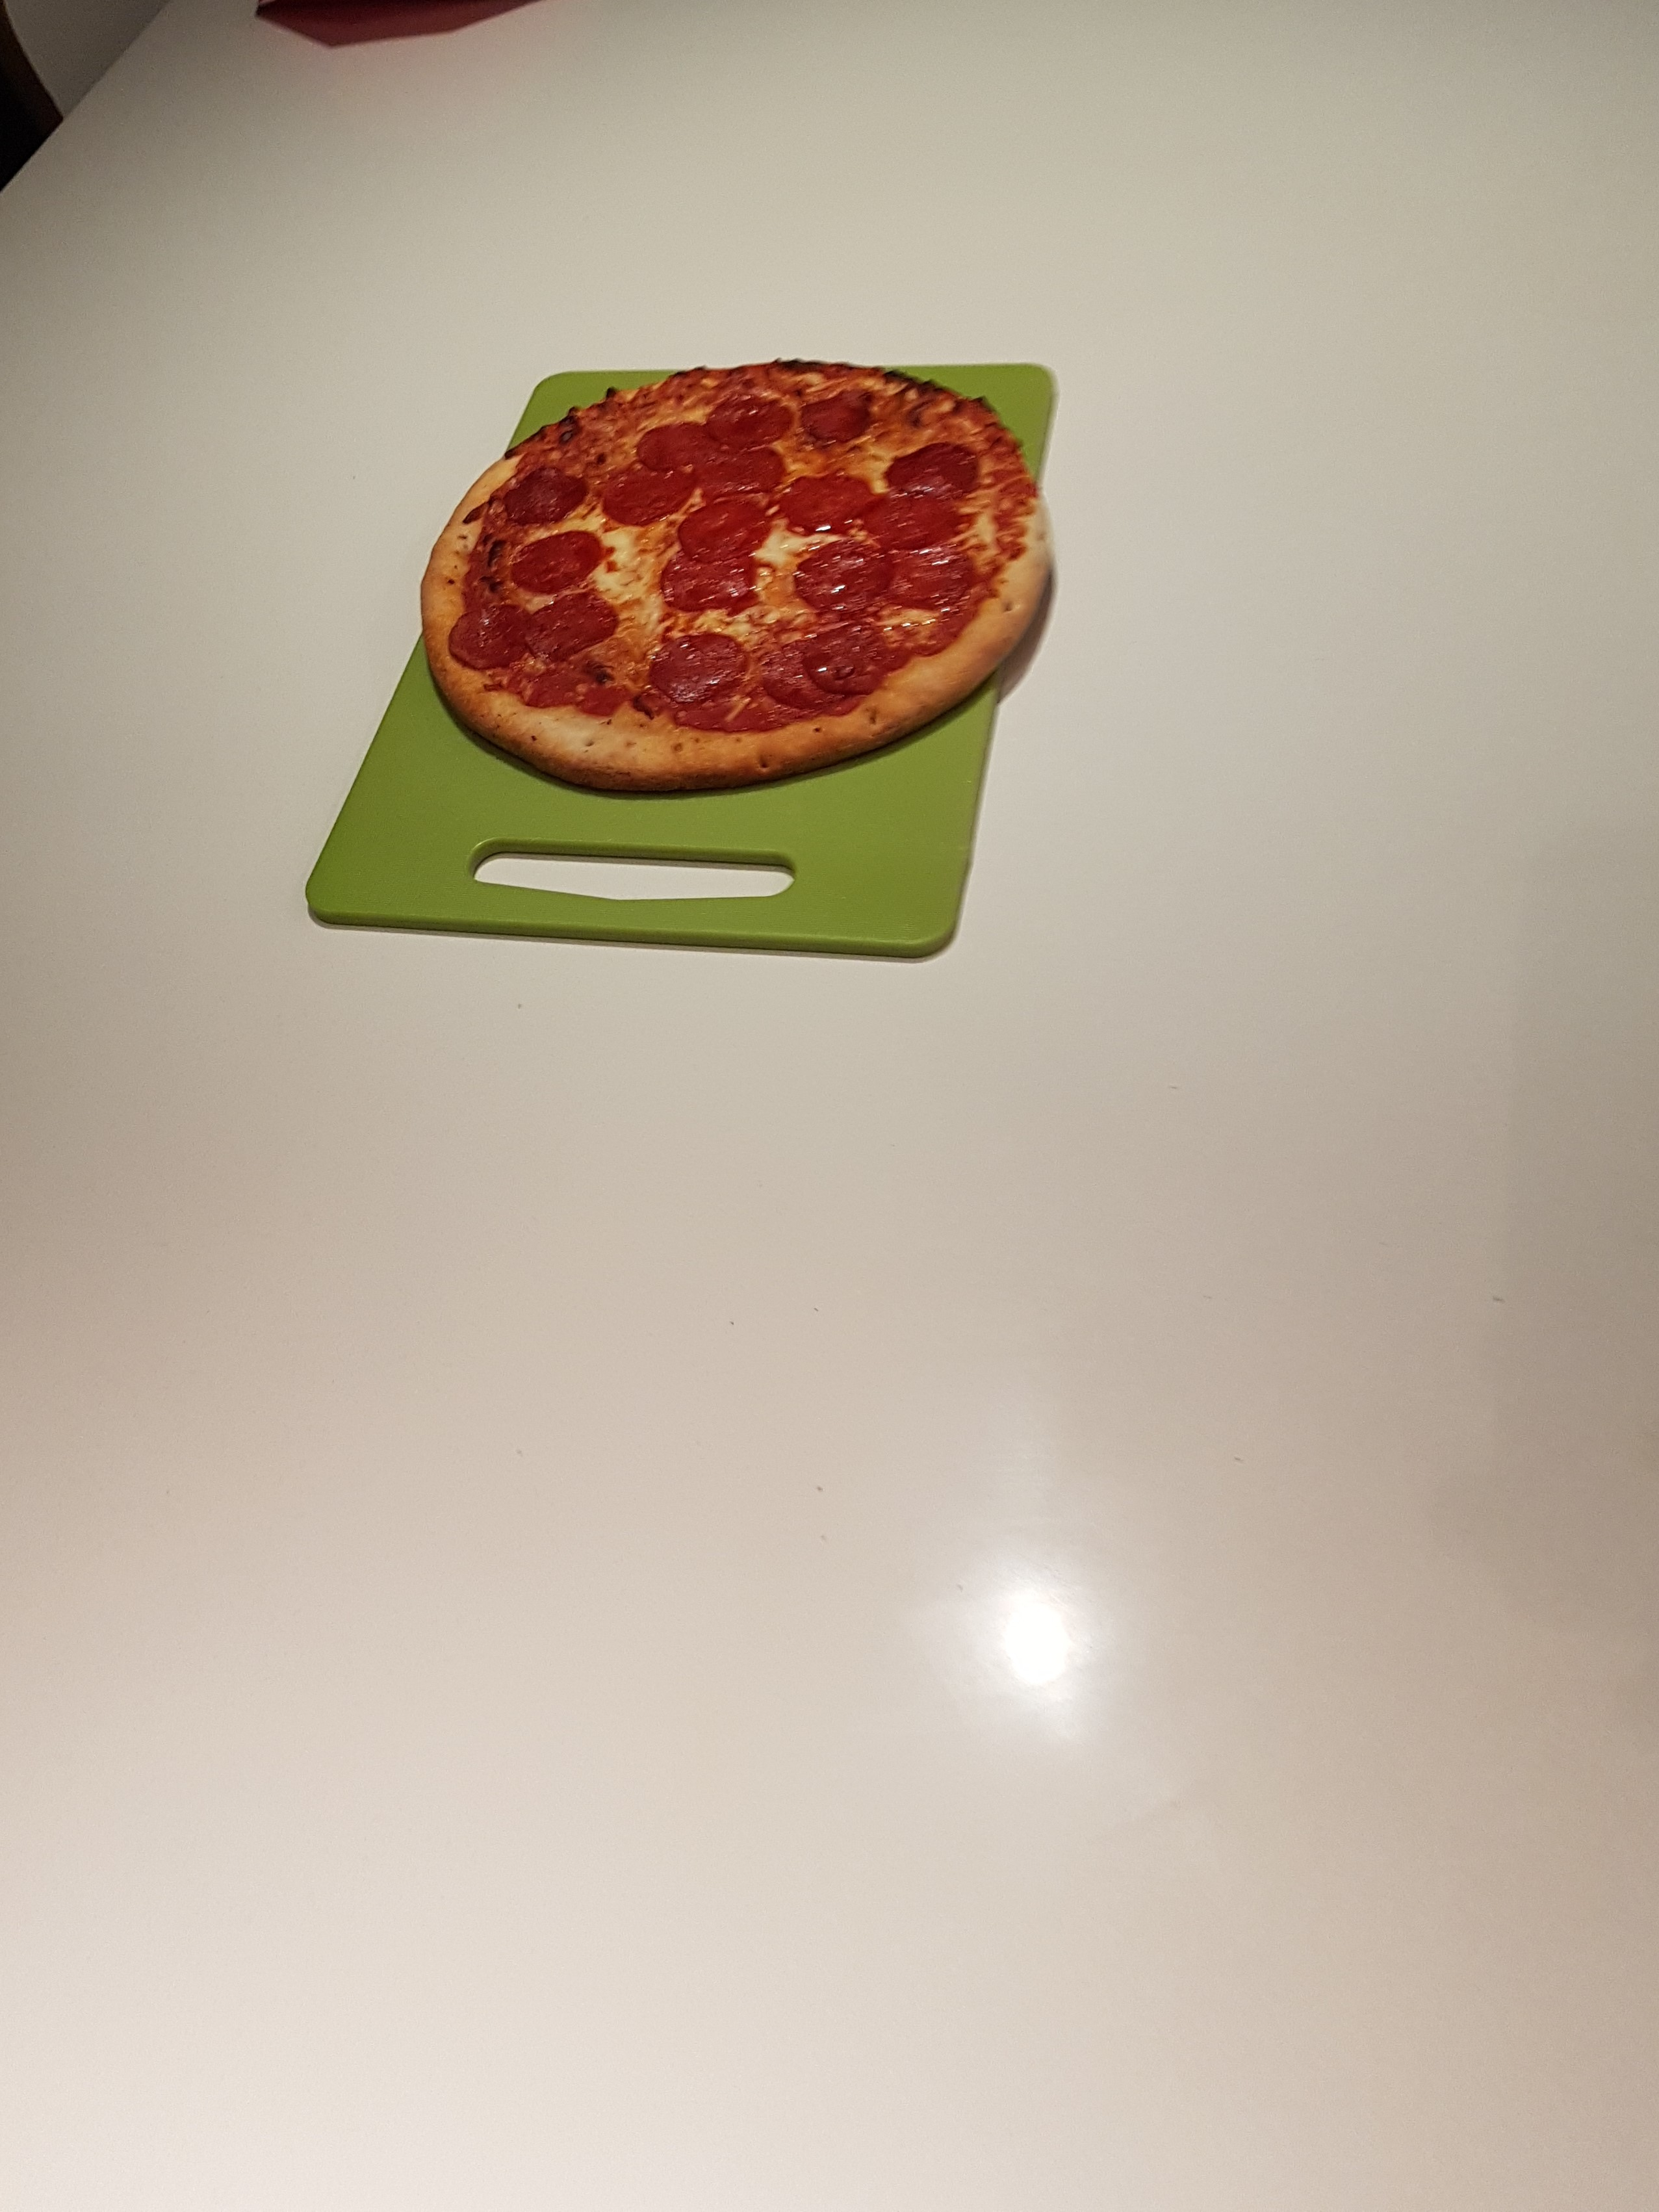
\includegraphics[scale=0.065]{pizza_unclassified} 
    \caption{Pizza not classified correctly by the model} 
  \label{fig:pizza_unclassified}
    \vspace{4ex}
  \end{minipage} 
\end{figure}

\subsection*{Analysis}
These poor results are not that surprising.
This is because we have many classes to train for, 101, and no parameter tuning has been carried out on the running of this code.
Figure \ref{fig:pizza_unclassified} was not classified correctly, this is most likely due to the fact that the pizza does not take up much of the image.



\section{Retrain with Extended Dataset}
\label{extended}
\subsection*{Overview}
For my fifth experiment, I decided to take inspiration from
\textcite{yanaiFood}, where pre-training was used training a model for food
classification. In order to achieve this, I retrained the final layer of the
Inception V3 model which was trained on the ImageNet dataset. This is called
Transfer Learning. I followed the tutorial by Google on the tensorflow website
for direction on this process \textcite{retrainInception}.

Firstly, in order to retrain the final layer of a model, a dataset must be
prepared in the correct way. I used the Food-101 dataset \textcite{food101}
which I will analyse in a later section. The dataset must be structured so that
there is a separated directory for each class with the directory name as the class
name. These directories should contain all the images for this class. 

Once this dataset has been set up correctly, a directory can be found on github
which contains the necessary files for this tutorial. When the directory has
been downloaded, the following command can be ran:
\begin{lstlisting}
python tensorflow/examples/image_retraining/retrain.py \ --image_dir
~/dataset_directory
\end{lstlisting}

The first thing that the script will do is create bottleneck files for the
images. A bottleneck is a term used to define the final layer before the output
layer. This is so that for each image, we do not have to push it through the
entire network during training \textcite{retrainInception}.

After, the bottlenecks are created, the training can be completed. The images
are split into three sub directories of training, testing and validation. By
default, these images are split into percentages of 80\%, 10\% and 10\%
respectively. The model is trained at a default of 4000 steps. 

At the final stage of the script, the model is run on a batch of test images not
yet seen and a final test accuracy is displayed. This can be seen in the Script
section below.

The command used for using this model once it is trained is:
\begin{lstlisting}
python tensorflow/examples/label_image.py --graph=/tmp/output_graph.pb
--labels=/tmp/output_labels.txt --input_layer=Mul --output_layer=final_result
--input_mean=128 --input_std=128 --image=~/image_directory
\end{lstlisting}

\subsection*{Network Architecture}
The Inception V3 model network architecture was used which consists of 22
layers.

\subsection*{Dataset}
The dataset used for this experiment is the Food-101 dataset \textcite{Food
101}. This dataset has 101 classes with 1000 images for each class.

\subsection*{Libraries}
Tensorflow and Numpy were used to run this scipt.

\subsection*{Script}
The following snippets of code are from the retrain.py script.

\begin{lstlisting}
# Add the new layer that we'll be training.
(train_step, cross_entropy, bottleneck_input, ground_truth_input,
final_tensor) = add_final_training_ops(
            len(image_lists.keys()), FLAGS.final_tensor_name,
            bottleneck_tensor,
            model_info['bottleneck_tensor_size'],
            model_info['quantize_layer'])
 
# Create the operations we need to evaluate the accuracy of our new layer.
evaluation_step, prediction = add_evaluation_step(
final_tensor, ground_truth_input)
 
# Merge all the summaries and write them out to the summaries_dir
merged = tf.summary.merge_all()
train_writer = tf.summary.FileWriter(FLAGS.summaries_dir + '/train',
                                     sess.graph)
 
validation_writer = tf.summary.FileWriter(
    FLAGS.summaries_dir + '/validation')
 
# Set up all our weights to their initial default values.
init = tf.global_variables_initializer()
sess.run(init)

\end{lstlisting}




\begin{lstlisting}
# We've completed all our training, so run a final test evaluation on
# some new images we haven't used before.
test_bottlenecks, test_ground_truth, test_filenames = (
    get_random_cached_bottlenecks(
        sess, image_lists, FLAGS.test_batch_size, 'testing',
        FLAGS.bottleneck_dir, FLAGS.image_dir, jpeg_data_tensor,
        decoded_image_tensor, resized_image_tensor, bottleneck_tensor,
        FLAGS.architecture))
test_accuracy, predictions = sess.run(
   [evaluation_step, prediction],
   feed_dict={bottleneck_input: test_bottlenecks,
        ground_truth_input: test_ground_truth})
tf.logging.info('Final test accuracy = %.1f%% (N=%d)' %
                (test_accuracy * 100, len(test_bottlenecks)))
\end{lstlisting}

\subsection*{Results}
The final test accuracy for this retrained model was 54.8\%.

For example, an image of pizza, see \ref{fig:pizza} was fed into the model with the followng results:
\begin{itemize}
    \item{pizza 0.925}
    \item{pancakes 0.008}
    \item{nachos 0.007}
    \item{beef carpaccio 0.006}
    \item{tiramisu 0.004}
\end{itemize}

\begin{figure}
     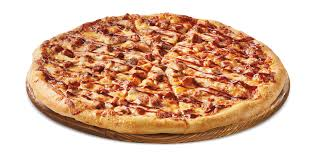
\includegraphics{pizza}
     \caption{Pizza}
     \label{fig:pizza}
\end{figure}

\subsection*{Analysis}


\section{Retrain with Parameter Tuning}
\label{parameterTuning}
\tocless\subsection{Objective}
Within the retrain.py script \parencite{retrainInception}, as mentioned in
previous experiments, there are various parameters that can be set and changed.
Various combinations of these parameters were changed to see if it would increase the
test accuracy of the model.

\begin{table}[h]
\centering
\caption{Retrain with Parameter Tuning}
\label{my-label}
\begin{tabular}{|l|p{8cm}|}
\hline
\textbf{Network Architecture} & Inception-V3           \\ \hline
\textbf{Dataset}              & Food-101+ dataset \\ \hline
\textbf{APIs and Libraries}   & TensorFlow and NumPy                                                       \\ \hline
\end{tabular}
\end{table}

\tocless\subsection{Script}
Script as seen in \ref{inception} but with some additions to calculate Top 5 accuracy as seen
in Figure \ref{lst:top5}.
Also documented is the code used to label a new image using the model (Figure \ref{lst:labelImage2}).

Figure \ref{lst:top5} takes 10 images for each class and runs each through the model.
The script then checks if the expected value is within the top 5 predictions returned from Figure \ref{lst:labelImage2}.
If it is the amount of correct top 5 predictions is incremented by one.
To calculate the Top-5 accuracy, the number of correct top-5 predictions is divided by the total number of images tested (10 images per class x number of classes) and multiplied by 100 for obtain a percentage value.


\begin{figure}[h]
\caption{Retrain Inception With Parameter Tuning Command}
\label{lst:retrainParameterCommand}
\begin{lstlisting}
python retrain_top5.py \ --image_dir
~/dataset_directory \ --how_many_training_steps 4000 \ --learning_rate 0.01 \
--testing_percentage 10 \ --validation_percentage 10
\end{lstlisting}
\end{figure}

Top 5 accuracy of the model was also calcultaed using the code below.
\begin{figure}[h]
\caption{Top-5 Accuracy Calculation}
\label{lst:top5}
\begin{lstlisting}[style=Python]
#Variables used to store a list of all classes, the amount of images tested,
# the amount of images with a top 5 accuracy and the sum of the highest probabilities
classes = list(image_lists.keys())
image_count = 0
top_5_count=0
total_of_top1_probs = 0
i = 0 
class_counter = 0

#Loops through all test images, selecting 10 images per class 
#and running them through the method in 'label_image.py'.
while(i < len(test_bottlenecks)):
  class_counter += 1
  
  if class_counter > 10:
    i = int(round((i + len(test_bottlenecks)/len(classes)) - 10))
    class_counter = 0
  else:
    image_count += 1
    results_from_classifier = label_image.runModel(test_filenames[i])
    results = results_from_classifier[0]
    probabilities = results_from_classifier[1]

    if classes[test_ground_truth[i]] in results:
      top_5_count += 1
    else:
      print("Expected:  " + classes[test_ground_truth[i]])
      for result in results:
        print("Classes: " + result)
      print("")

    total_of_top1_probs += max(probabilities)
    i = i + 1
print(str(top_5_count))
average_probabilities = total_of_top1_probs/(len(classes*10))

#Prints out the amount of test images used, the top 5 accuracy
# and the average probability of predictions.
print("Amount of test images: " + str(image_count))
print("Top 5 Accuracy: " + str((top_5_count/image_count)*100))
print("Average probability: " + str(average_probabilities))
\end{lstlisting}
\end{figure}

\begin{figure}[h]
\caption{Label Image - adapted from \parencite{retrainInception}}
\label{lst:labelImage2}
\begin{lstlisting}[style=Python]
def runModel(file_name):
  model_file = \
    "/tmp/output_graph.pb"
  label_file = "/tmp/output_labels.txt"
  input_height = 299
  input_width = 299
  input_mean = 128
  input_std = 128
  input_layer = "Mul"
  output_layer = "final_result"

  graph = load_graph(model_file)
  t = read_tensor_from_image_file(file_name,
                                  input_height=input_height,
                                  input_width=input_width,
                                  input_mean=input_mean,
                                  input_std=input_std)

  input_name = "import/" + input_layer
  output_name = "import/" + output_layer
  input_operation = graph.get_operation_by_name(input_name)
  output_operation = graph.get_operation_by_name(output_name)

  with tf.Session(graph=graph) as sess:
    results = sess.run(output_operation.outputs[0],
                      {input_operation.outputs[0]: t})
  results = np.squeeze(results)

  top_k = results.argsort()[-5:][::-1]
  labels = load_labels(label_file)
  
  setIndex = False

  top5_results = [None] * 5
  index = 0
  for i in top_k:
    top5_results[index] = labels[i]
    index += 1

  final_results = [top5_results, results]
  return final_results
\end{lstlisting}
\end{figure}

Some further parameters could be set such as:
\begin{itemize}
	\item{--flip\_left\_right}
	\item{--random\_crop}
	\item{--random\_scale}
	\item{--random\_brightness}
\end{itemize}

\begin{figure}[h]
    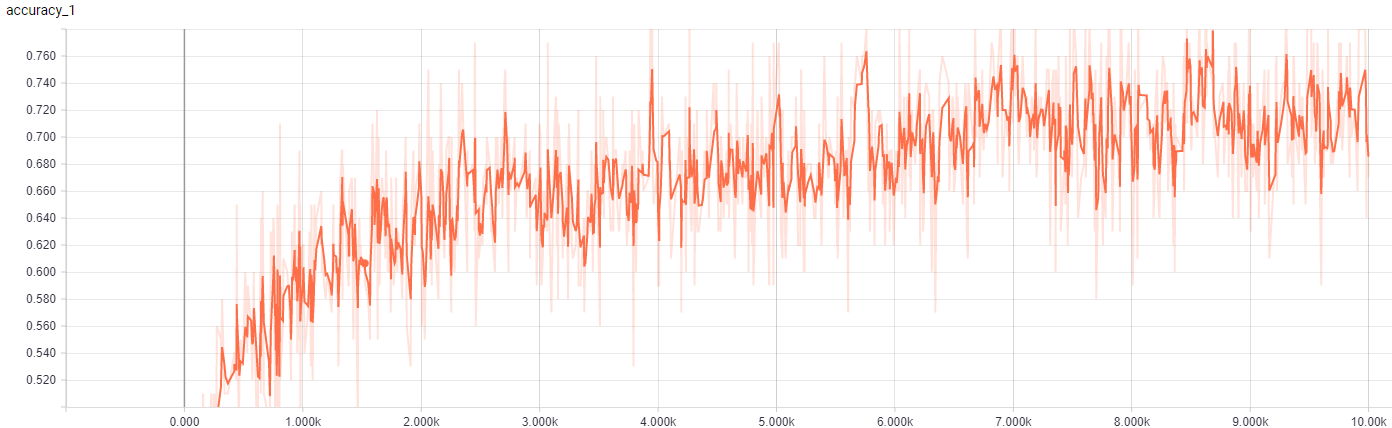
\includegraphics[scale=0.4]{model_test}
     \caption{Graph of accuracy of the test dataset during training}
     \label{fig:model_train_test}
\end{figure}

\begin{figure}[h]
    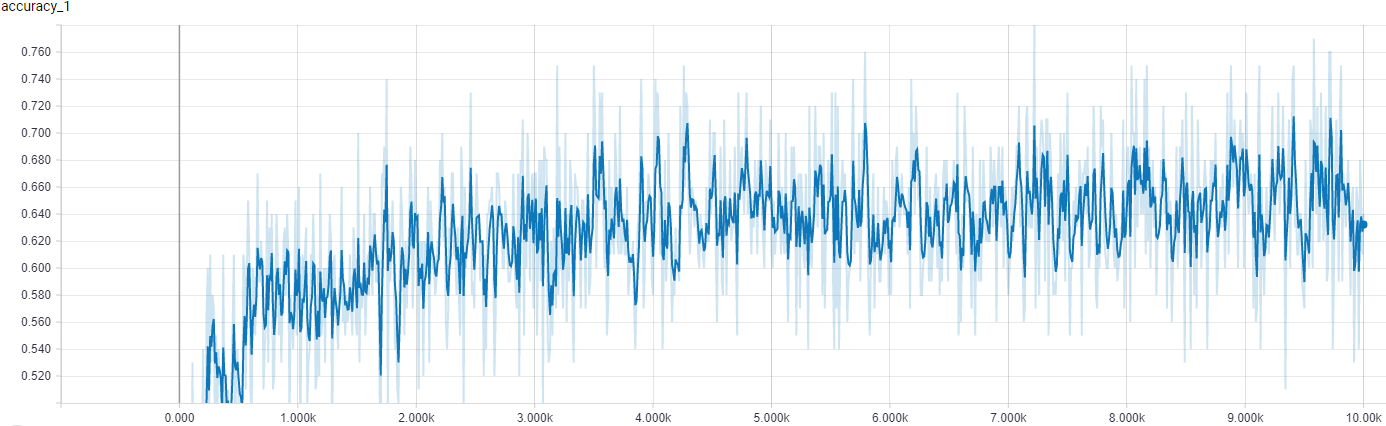
\includegraphics[scale=0.4]{model_val}
     \caption{Graph of accuracy of the validation dataset during training}
     \label{fig:model_train_val}
\end{figure}

\begin{figure}[h]
    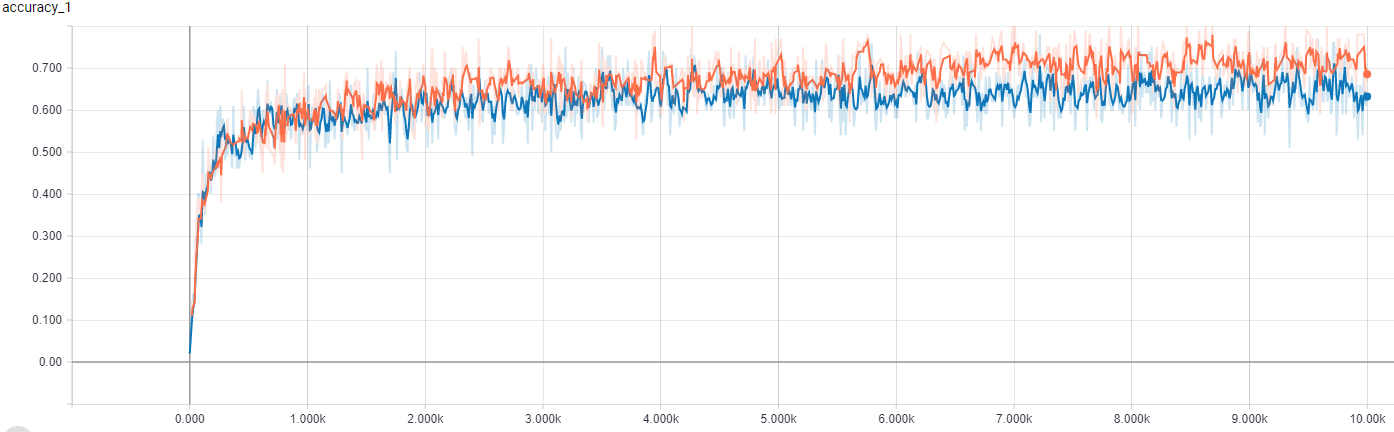
\includegraphics[scale=0.4]{test_val_accuracy}
     \caption{Comparison of accuracy}
     \label{fig:test_val_accuracy}
\end{figure}

\begin{figure}[h]
    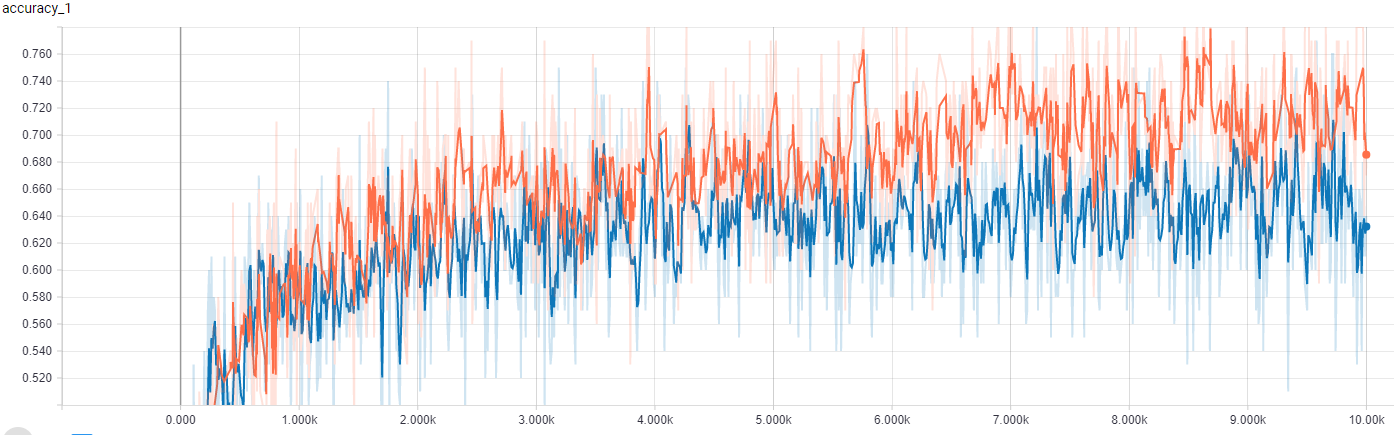
\includegraphics[scale=0.4]{test_val_accuracy_refined}
     \caption{Comparison of accuracy}
     \label{fig:test_val_accuracy_refined}
\end{figure}


\begin{table}[]
	\centering
	\caption{Comparison of parameters}
	\label{parameter_tuning_table}
	\begin{tabular}{|p{3cm}|l|l|l|l|l|}
  \hline
		\textbf{Parameter Tuning} & \textbf{Steps} & \textbf{Learning Rate} & \textbf{Test} \% & \textbf{Validation} \% &
		\textbf{Results} \\ \hline
		Configuration 1  & 8,000  & 0.01       & 10 & 10       &
		59.1\%  \\ \hline
		Configuration 2  & 8,000  & 0.10           & 10 & 10       &
		65.8\%  \\ \hline
		Configuration 3  & 10,000 & 0.10           & 10 & 10       &
		66.3\%  \\ \hline
		Configuration 4  & 12,000 & 0.10           & 10 & 10       &
		66.6\%  \\ \hline
		Configuration 5  & 10,000 & 0.20           & 10 & 10       &
		66.0\%  \\ \hline
		Configuration 6  & 10,000 & 0.10           & 15      & 15            &
		66.3\%  \\ \hline
	\end{tabular}
\end{table}

\tocless\subsection{Results}
The results of each set of parameters can be seen in Table
\ref{parameter_tuning_table}.
Using the parameters of 10,000 steps, and a learning rate of 0.1 and therefore a final test accuracy of 66.3\%, the model achieved a Top 5 accuracy of 85.96\%.
This Top-5 accuracy was calculated from 1090 images in the test dataset and the average probability of the predictions were at 0.62.
The 95\% confidence interval of the Top-1 accuracy of this model is between 57.4\% and 75.2\%.


\tocless\subsection{Analysis}
The set of parameters that seem to be the most
effective are 10,000 steps with a 0.1 learning rate. Graphs of this model can be
seen in Figures \ref{fig:model_train_val} and \ref{fig:model_train_test}. These
are based on the validation set and then the test set respectively. A side by
side comparison can also be seen in Figures \ref{fig:test_val_accuracy} and
\ref{fig:test_val_accuracy_refined} where orange is for during training and blue
for the validation set.

There were two separate factors that each increased classification accuracy of
about 5\% each. These were training steps and learning rate.

Training steps are related to the number of images so before, when the training
steps were at 4,000, not all of the training images were being used. As the steps were increased
twofold we saw a 3.8\% increase in accuracy.

Another parameter that increased accuracy significantly was learning rate. The
default learning rate is 0.01 which was increased to 0.1. This resulted in an
increase of 6.7\%. This is most likely since we are only
looking at the last layer, we can afford to change the weights more
significantly.

The Top 5 accuracy of the model was quite good but it was not run on the same number of images as the final test accuracy.
This is beacuse TensorFlow does not have an API for calculating Top 5 accuracy.
As a result, it had to be calculated manually and this is very time intensive.
The average probability of 0.62 is also quite close to the overall Top 1 accuracy which may imply some correlation between the two but this is merely speculation.

\afterpage{\clearpage}


\section{MobileNet}
\label{mobilenet}
\tocless\subsection{Objective}
Since the end goal for this project is to have a smartphone
application that a user can use to keep track of their calorie measurement,
there are a couple of options in how to achieve this. Firstly, an image can be
taken on the phone and sent to a server to run a classification algorithm.
Secondly, a model can be stored on the phone for computation. Transfer learning was once again used but on a different, smaller architecture called MobileNet \parencite{mobilenet}.

\begin{table}[h]
\centering
\caption{MobileNet}
\label{my-label}
\begin{tabular}{|l|p{8cm}|}
\hline
\textbf{Network Architecture} & MobileNet           \\ \hline
\textbf{Dataset}              & Food-101+ dataset \\ \hline
\textbf{APIs and Libraries}   & TensorFlow and NumPy                                                       \\ \hline
\end{tabular}
\end{table}

\tocless\subsection{Script}
The retrain.py script \parencite{retrainInception} was used, with a different
command parameter.

\begin{lstlisting}[style=Command]
python tensorflow/examples/image_retraining/retrain.py \ --image_dir
~/dataset_directory \ --architecture mobilenet_1.0_224 \
--how_many_training_steps 10000 \ --learning_rate 0.1
\end{lstlisting}

\tocless\subsection{Results}
The final test accuracy of this model came to 50.2\%.

\tocless\subsection{Analysis}
There was a decrease of 16.1\% in this model to the highest accuracy from
\ref{mobilenet}. This is due to the smaller architecture which is aimed to be faster
and smaller with an expected decrease in accuracy.


\section{Food 101 subset}
\label{subset}
\subsection*{Objective}
In many of the papers that have been researched where food image classification was carried out, they attempted to classify a lot less than 108 food types as has been the case for experiments previously shown.
\parencite{novelSVM} used 12 classes, \parencite{pouladzadeh2014measuring} had 15, \parencite{LSL_2015} attempted to classify 11 classes of food, 20 classes were used in \parencite{chen2010toward} and \parencite{snap} predicted 15 classes.
Due to the lower number of classes in these papers, it was decided to retrain inception on a subset of the food-101 extended dataset to benchmark results.
13 classes were selected from food-101 for training.

\subsection*{Network Architecture}
Retrained Inception model.

\subsection*{Dataset}
A subset of the Food 101 dataset was used for this experiment \parencite{food101}.

\subsection*{Results}
A Final test Accuracy of 92.6\% was recorded for this experiment which performs quite high in comparison to the data in Table \ref{classes_accuracy}.
A Top 5 accuracy of 100\% was calculated with an average prediction probability of 0.89 using 130 images.
This was calculated using the script defined in \ref{parameterTuning}.

\begin{table}[]
\centering
\caption{Accuracy of other studies}
\label{classes_accuracy}
\begin{tabular}{|l|l|l|}
\hline
\textbf{Reference}                       & \textbf{Classes} & \textbf{Accuracy}      \\ \hline
Novel SVM                       & 12      & 92.6\%        \\ \hline
Measuring Calorie and Nutrition & 15      & 90.4\%       \\ \hline
Large Scale Learning            & 11      & 78.0\%          \\ \hline
Toward Dietary Assessment       & 20      & 91.7\% \\ \hline
Snap-n-eat                      & 15      & 85.0\%         \\ \hline
\end{tabular}
\end{table}

\subsection*{Analysis}
It would make sense the accuracy of our model would increase when the number of classes are reduced as the margin of error is decreased.
The Top 5 accuracy of the model was very successful.
There were only 10 images per class tested though, totaling at 130 images so if the number of images increased, this accuracy would probably decrease slightly.
If the code is run again, the same results cannot even be replicated for sure.
On another run of this code a Top 5 accuracy of 96\% was recorded.
While this is still a very good accuracy, it does not compare to the first run of the script.

\chapter{Analysing the Trained Model}

\section{Sliding Window}
\label{slidingWindow}
\subsection*{Overview}
In the preious experiments, I have looked at the one-shot approach to food image
classification. That is, the model will give a prediction of the most likely
food item in that image. This is a problem when there are multiple food in an
image, see \ref{fig:fruit}. There are a few options to combat this problem. Firstly, I could detect
objects in the image, segment the image according to these objects and then run
each segment through the model. A simple approach to this would be to segment
the image into a number of sections and then run each section through the model.
In order to follow the latter approach, I used a sliding window approach. This
sliding window would move across the image and classify the segment of the image
in the window. I had three options for window sliding shape as defined by a
command line argument.

\begin{lstlisting}
python sliding_window.py --image=~/image_dir --window_shape grid
\end{lstlisting}

There are three options for window shape:
\begin{itemize}
	\item{Grid based window as per \ref{fig:fruitGrid}}
	\item{Row based window as per \ref{fig:fruitRow}}
	\item{Column based window as per \ref{fig:fruitColumn}}
\end{itemize}

\begin{figure}
    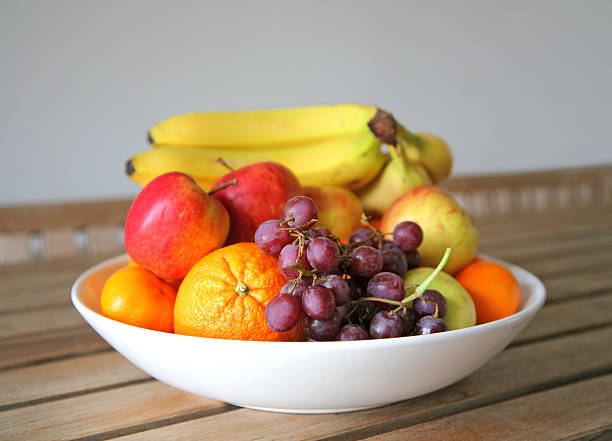
\includegraphics[scale=0.5]{fruit}
    \caption{Bowl of fruit}
    \label{fig:fruit}
\end{figure}

\begin{figure}
    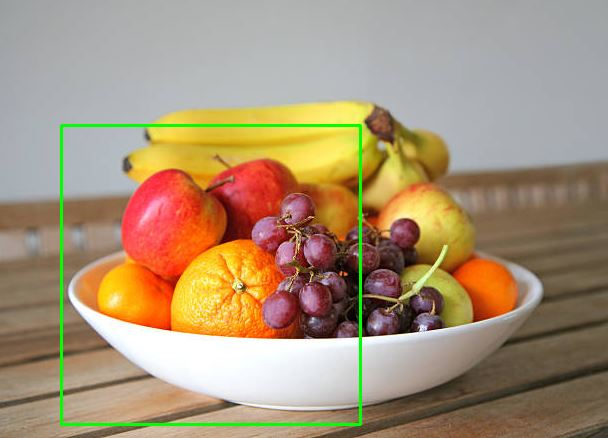
\includegraphics[scale=0.5]{fruitGrid}
	\caption{Grid based window}
    \label{fig:fruitGrid}
\end{figure}

\begin{figure}
    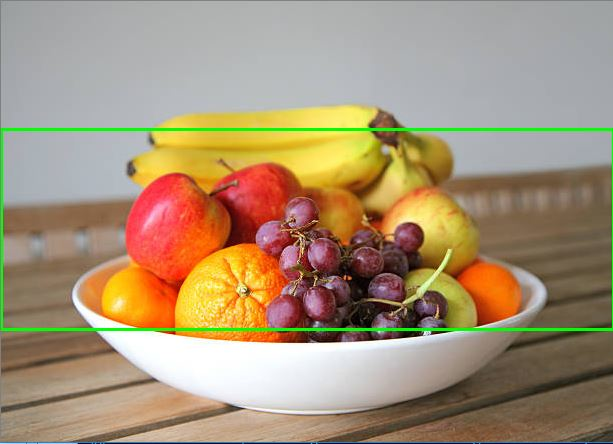
\includegraphics[scale=0.5]{fruitRow}
    \caption{Row based window}
    \label{fig:fruitRow}
\end{figure}

\begin{figure}
    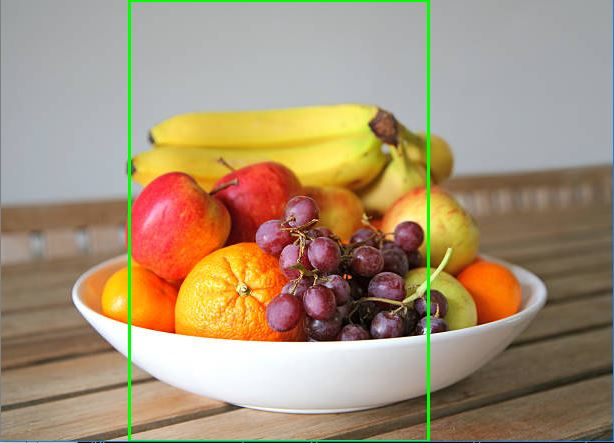
\includegraphics[scale=0.5]{fruitColumn}
    \caption{Column Based Window}
    \label{fig:fruitColumn}
\end{figure}

\begin{figure}
    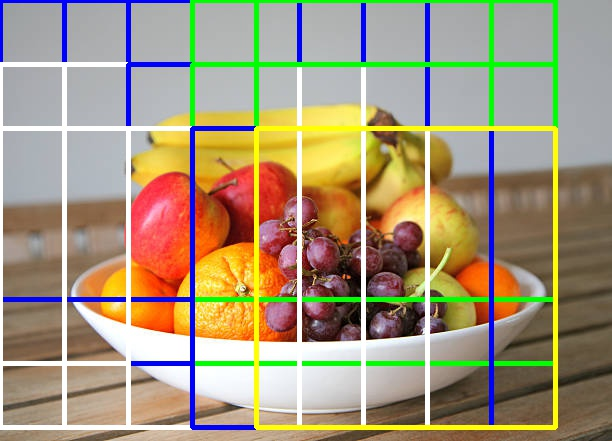
\includegraphics[scale=0.5]{fruitCO}
    \caption{Fruit with Color Overlay}
    \label{fig:fruitOverlay}
\end{figure}

\subsection*{Libraries}
For this experiment Tensorflow provided the classification of each segment while
also helping with resizing along with Numpy. OpenCv was used to implement the
sliding window as per \textcite{slidingWindowTut}

\subsection*{Script}
There were four main elements to the script. Firstly, extracting a window to be
classified. Secondly, resizing the image to be compatible with the Tensorflow
model. Thirdly, running the window through the Tensorflow model and finally
saving a new image with a coloured overlay of classifications.

\subsubsection*{Extracting the window from the image}
\begin{lstlisting}
# loop over the image pyramid
for resized in pyramid(image, scale=1.5):
		# loop over the sliding window for each layer of the pyramid
		for (x, y, window) in sliding_window(resized, stepSize=32, windowSize=(winW, winH)):
			# if the window does not meet our desired window size, ignore it
				if window.shape[0] != winH or window.shape[1] !=winW:
					continue
\end{lstlisting}


\begin{lstlisting}
def sliding_window(image, stepSize, windowSize):
	# slide a window across the image
	for y in xrange(0, image.shape[0], stepSize):
		for x in xrange(0, image.shape[1], stepSize):
			# yield the current window
			yield (x, y, image[y:y + windowSize[1], x:x + windowSize[0]])
\end{lstlisting}

\subsubsection*{Resizing the window}
\begin{lstlisting}
window = cv2.resize(window, (299, 299))
\end{lstlisting}

\begin{lstlisting}
resized_image = tf.reshape(image, [1, input_height, input_width, 3])
resized = tf.image.resize_area(resized_image, [input_height, input_width])
normalized = tf.divide(tf.subtract(resized, [input_mean]), [input_std])
\end{lstlisting}

\subsubsection*{Running the Tensorflow model}
\begin{lstlisting}
with tf.Session() as sess:
	numpy_image = sess.run(normalized)

with tf.Session(graph=graph) as sess:
    results = sess.run(output_operation.outputs[0],
                      {input_operation.outputs[0]: numpy_image})
	probabilities = np.squeeze(results)
\end{lstlisting}

\subsubsection*{Saving the image with colour overlay}
As seen in Figure \ref{fig:fruitOverlay}, each square represents a window and
each colour is for a different classification. Blue is for an apple, yellow for
banana, green for grape, white for orange and black if an unexpected prediction
is made.

\begin{lstlisting}
cv2.rectangle(display_image, (x, y), (x + winW, y + winH), colour_dict.get(top1,
(0,0,0)), 4)
\end{lstlisting}

\subsection*{Results}
\subsubsection*{Grid based window}
The grid based window resulted in fifteen separate classification. As seen in
\ref{fig:fruit}, there are multiple fruits in the image. Of these fruits, our
model is trained on four, apple, banana, orange and grapes. This method
classified all four to Top-1 accuracy at least once each. This method took 42.8
seconds to run.

\begin{table}[]
	\centering
	\caption{My caption}
	\label{my-label}
	\begin{tabular}{ll}
		Food type & No. of Top-1 Classifications \\
		Apple     & 5                      \\
		Banana    & 1                      \\
		Grape     & 4                      \\
		Orange    & 5                     
	\end{tabular}
\end{table}

\begin{table}[]
	\centering
	\caption{My caption}
	\label{rowWindowTable}
	\begin{tabular}{ll}
		Food type & No. of Top-1 Classifications \\
		Apple     & 1                      \\
		Banana    & 0                      \\
		Grape     & 0                      \\
		Orange    & 0                      \\
		Other     & 3                     
	\end{tabular}
\end{table}

\begin{table}[]
	\centering
	\caption{My caption}
	\label{colWindowTable}
	\begin{tabular}{ll}
		Food type & No. of Top-1 Classifications \\
		Apple     & 3                      \\
		Banana    & 1                      \\
		Grape     & 0                      \\
		Orange    & 0                      \\
		Other     & 1                     
	\end{tabular}
\end{table}

\subsubsection*{Row based window}
The row based method resulted in four predictions as follows in
\ref{rowWindowTable}. Out of these four predictions, only one classified a known
fruit at Top-1 accuracy, an apple. An apple was also predicted to Top-5 accuracy
in another instance. The runtime of this method was 16.1 seconds.

\subsubsection*{Column based window}
The column based window approach had five total predictions and ran for a total
of 13 seconds. As seen in \ref{colWindowTable}, two out of four known fruits
were classified to a Top-1 accuracy with all other fruits predicted to Top-5
accuracy. Only one Top-1 prediction did not contain a correct fruit.

\subsection*{Empirical Analysis}
These results are very interesting because while a banana was only predicted to
Top-1 accuracy once in grid based, once in column based and zero times in row
based, if the whole image is ran through the model, a banana is at the Top-1 accuracy.


























\section{Recursive Refinement}
\label{RR}
\tocless\subsection{Objective}
After the sliding window code was run on Figure \ref{fig:fruit} in \ref{slidingWindow},
it was observed that a sliding window was predicting grapes correctly in
regions that contained a bunch of grapes. Since it would make sense that the
model would be able detect an individual grape, it was decided that
recursive refinement would be ran on a window that contained a grape. Due to the model
requiring a 299 x 299 image size, the window could only be refined once as
very small segments could not be resized up to 299 x 299. A window of 70 x 70 size was used.

\tocless\subsection{Script}
As you would think with recursive refinement, a recursive function would be used,
but this was unnecessary due to image size restrictions. Instead, a
conditional for loop was added to the existing code to break a window down further i.e. perform a sliding window approach on a window.
This can be seen in Figure \ref{lst:rrCode}.

\begin{figure}[h]
\caption{Recursive Refinement Code}
\label{lst:rrCode}
\begin{lstlisting}[style=Python]
if top1 == "grape" and window_shape == "grid" and rr_grape:
			for (x_grape, y_grape, grape_window) in sliding_window(window_resized, stepSize=64, windowSize=(70, 70)):
				#reshape to square
				grape_window_resized = cv2.resize(grape_window, (299, 299))
				top1_grape = subSample.classify(grape_window_resized, window_shape)
				if top1_grape == "grape":
					cv2.rectangle(display_image, (x_grape + x, y_grape + y), (x_grape + x + 70, y_grape + y + 70), colour_dict.get(top1, (0,0,0)), 4)
					#cv2.imshow("Window", grape_window_resized)
					cv2.waitKey(1)
time.sleep(0.025)
\end{lstlisting}
\end{figure}

\begin{figure}[h]
\centering
    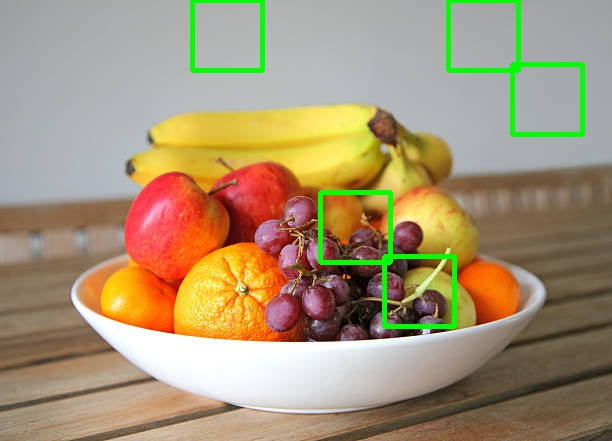
\includegraphics[scale=0.4]{fruit_rr}
      \caption{Recursive refinement 1}
      \label{fig:rr1}
\end{figure}

\tocless\subsection{Results}
Some very similar results were recorded on three separate images. Two new images are seen
here which we will explore in future experiments. In all three images, while the script
is calculating some expected predictions, grapes are being classified in locations
that have nothing resembling a grape. These can be viewed in Figures
\ref{fig:rr1}, \ref{fig:rr2} and \ref{fig:rr3}.

\tocless\subsection{Analysis}
The instances where false positives were recorded may indicate issues with the recursive refinement approach as every window must be classified and it is possible that this just happens to be a grape in some instances.
Further analysis to why this may be occurring is outlined in the section \ref{rrAnalyse}.

\begin{figure}
\centering
    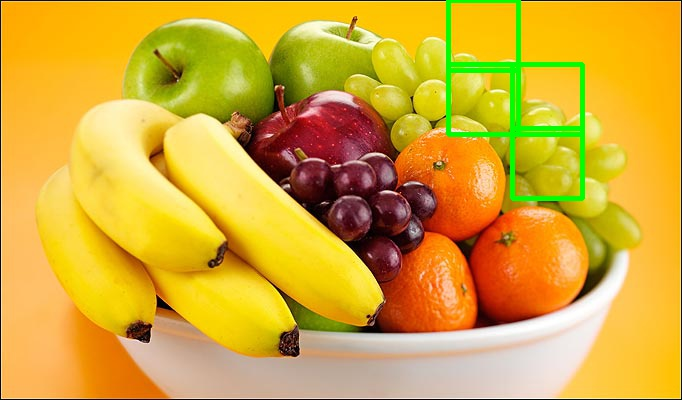
\includegraphics[scale=0.2]{newfruit_rr_grid}
      \caption{Recursive refinement 2 - sourced from http://www.travispta.org/}
      \label{fig:rr2}
\end{figure}

\begin{figure}
\centering
    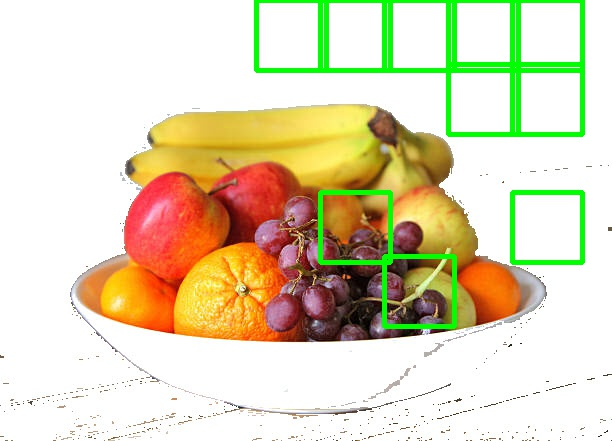
\includegraphics[scale=0.3]{processed_image}
      \caption{Recursive refinement 3}
      \label{fig:rr3}
\end{figure}



\section{Impact of Backround}
\label{background}
\tocless\subsection{Objective}
As we can see in section \ref{slidingWindow}, using sliding windows to classify many sections
of an image, there were some cases where some unexpected predictions were made.
Due to this, the decision was made to analyse the effect the background of the
image on its classification. The sliding window code was then ran on a new
image. This new image was the same fruit bowl as used previously but the
background was filled in as white as per Figure \ref{fig:filledFruit}.

\begin{figure}[h]
\centering
    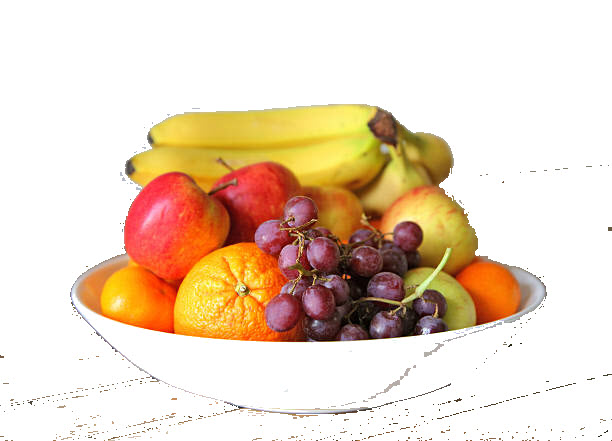
\includegraphics[scale=0.75]{fruitFillBg}
    \caption{Bowl of fruit with background removed}
    \label{fig:filledFruit}
\end{figure}

\begin{table}[h]
    \centering
    \caption{Comparison of fruit image sliding window results with and without
    background}
    \label{comparisionFruitTable}
    \begin{tabular}{|l|l|l|l|p{1.25cm}|p{1.25cm}|p{2cm}|}
    \hline
        \textbf{Food type} & \textbf{Grid} & \textbf{Row} & \textbf{Column} & \textbf{White Grid} & \textbf{White Row} & \textbf{White Column} \\ \hline
        Apple     & 5    & 1   & 3      & 10          & 0          & 4
        \\ \hline
        Banana    & 1    & 0   & 1      & 0           & 0          & 0
        \\ \hline
        Grape     & 4    & 0   & 0      & 1           & 0          & 1
        \\ \hline
        Orange    & 5    & 0   & 0      & 3           & 0          & 0
        \\ \hline
        Other     & 0    & 3   & 1      & 1           & 4          & 0  \\ \hline           
    \end{tabular}
\end{table}

\tocless\subsection{Results}
\tocless\subsubsection{Grid}
For grid-based sliding window approach, the results turned out to be less
successful than with the background. In this experiment, fourteen out of fifteen
of top-1 classification were of an expected food type rather than fifteen out of
fifteen with the background present. We expected the food types of apple,
orange, grape and banana to appear in this image but while a banana was detected
to a top-5 accuracy on a few occasions it was never predicted to a top-1
accuracy. The contrast between the image results can be seen in Table
\ref{comparisionFruitTable}.

\tocless\subsubsection{Row}
The row-based sliding window again had worse result than its counterpart, with
zero out of four correct classifications as opposed to one. In this case, an
orange appeared at top-5 accuracy once. The most common prediction was ice-cream
which appeared at top-1 accuracy in three out of four instances.

\tocless\subsubsection{Column}
In contrast to our previous two methods of sliding window, this method
outperformed its counterpart with correct predictions of all five windows while
before we only had four out of five. In this experiment, an apple was predicted
four times and a grape once, with all correct fruits appearing to top-5
accuracy.

\tocless\subsection{Analysis}
Surprisingly, removing the background of the image reduced the prediction
accuracy.
Many white foods were classified instead which makes sense due
the impact of colour expected.


\section{Alternative Test Image}
\label{alternative}
\begin{figure}
    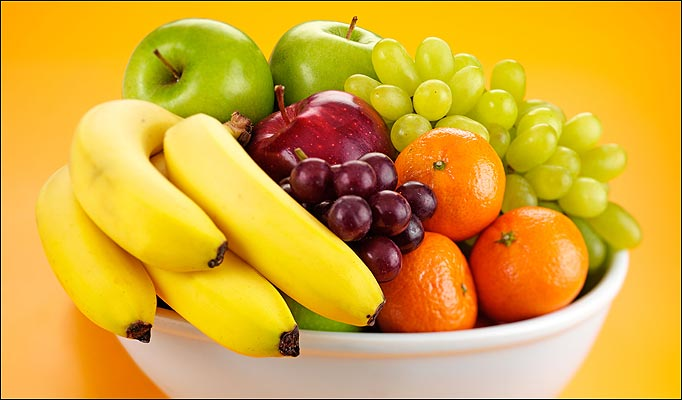
\includegraphics[scale=0.5]{fruitbowl2}
    \caption{Alternative Bowl of fruit}
    \label{fig:newFruit}
\end{figure}

\begin{table}[]
    \centering
    \caption{Comparison of fruit bowl images}
    \label{newFruitTable}
    \begin{tabular}{|l|l|l|l|l|l|l|}
    \hline
        \textbf{Food type} & \textbf{Grid} & \textbf{Row} & \textbf{Column} & \textbf{New Grid} & \textbf{New Row} & \textbf{New Column} \\ \hline
        Apple     & 5    & 1   & 3      & 4        & 1       & 0          \\ \hline
        Banana    & 1    & 0   & 1      & 5        & 0       & 5          \\ \hline
        Grape     & 4    & 0   & 0      & 2        & 1       & 0          \\ \hline
        Orange    & 5    & 0   & 0      & 0        & 0       & 0          \\ \hline
        Other     & 0    & 3   & 1      & 1        & 2       & 1         \\ \hline
    \end{tabular}
\end{table}

\subsection*{Overview}
In our previous sliding window oriented experiments, we had only used a
single image. In order to see whether this image had biases unknown
to us, another fruit bowl image had to be tested. This image was selected as
fruit took up a larger portion of the image as seen in Figure \ref{fig:newFruit}.

\subsection*{Results}
\subsubsection*{Grid}
The performance of this experiment was slightly worse than with the previously
used image. When the grid based sliding window was executed on Figure
\ref{fig:newFruit}, fourteen out of fifteen predictions had an expected value.
Out of the fourteen predictions orange was not predicted to top-1 accuracy at
all. This can be seen, in comparison to previously used image, in Table
\ref{newFruitTable}.

\subsubsection*{Row}
In the column based window for the new fruit image, the results were not very
successful as has been the trend for most row based classification. Two out of
four predictions had an expected value at top-1 accuracy.

\subsubsection*{Column}
The column based approach had a similar result to its counterpart in that only
one of its predictions was unexpected. Although, due  to the size of the new
image, another column was created and thus has a better overall accuracy.

\subsection*{Empirical Analysis}
A possible reason that an orange was not classified in any of these images is
because in Figure \ref{fig:newFruit}, a more mandarin food is displayed.


\section{Analysing Results of Recursive Refinement Further}
\label{rrAnalyse}
\tocless\subsection{Objective}
In Section \ref{RR}, some false positives were obtained when attempting to run recursive refinement on an image with grapes in it.
Originally it was meant to see if individual grapes could be recognised.
On evaluation of the images used for training, it was found that bunches of grapes were used for training, not individual grapes.
Therefore, the results expected where never feasibly going to be obtained.
Even though this was the case, the script resulted in finding grapes in portions of the background, as seen in Figure \ref{fig:rr1}.
The purpose of this experiment is to investigate why this is occurring.
A new image of a fruit bowl (Figure \ref{fig:fruitFromPhone}), taken on a mobile phone was selected for this experiment.
The image was used to run the script as defined in \ref{RR} but on two separate models.
The model with tuned parameters, trained on 108 classes, with a final test accuracy of 66.3\% and the model trained on 13 classes, with a final accuracy of 92.6\%.

\begin{figure}[h]
\centering
    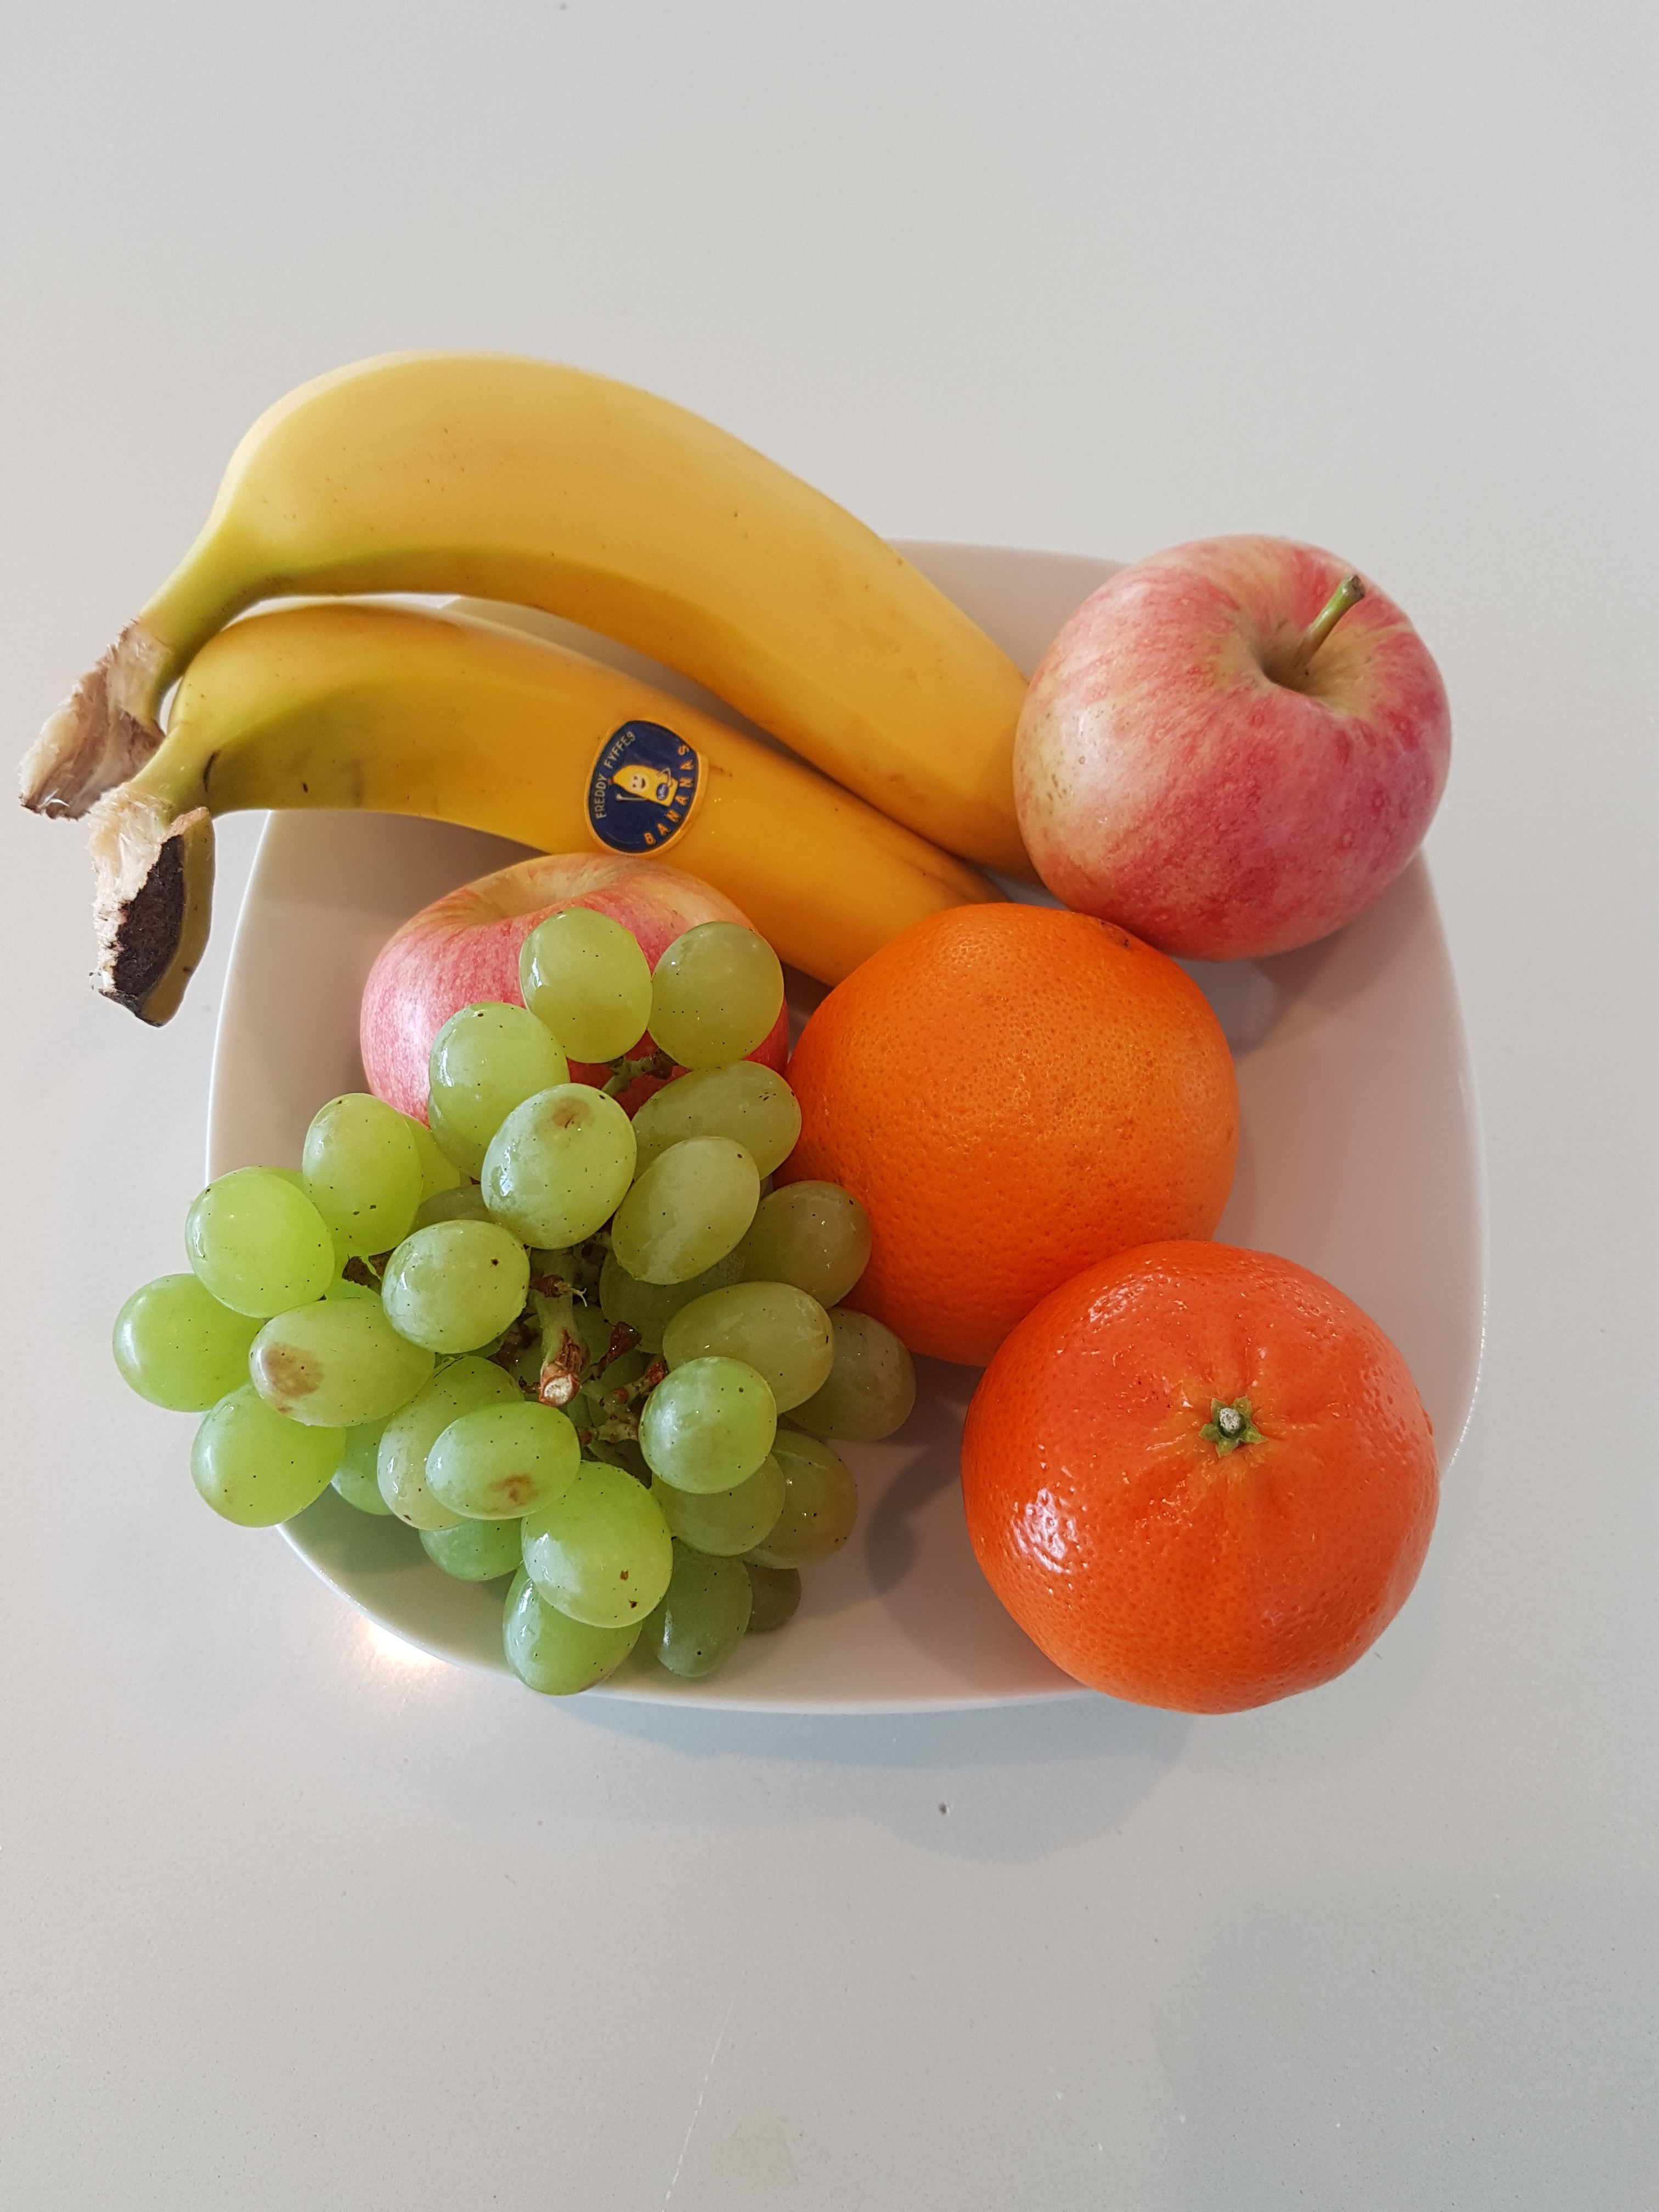
\includegraphics[scale=0.05]{fruitFromPhone}
      \caption{Fruit image taken on a mobile phone}
      \label{fig:fruitFromPhone}
\end{figure}

\tocless\subsection{Results}
The outputs of the script can be seen in Figure \ref{fig:fruitRR13} and Figure \ref{fig:fruitRR108}. The output using the model trained on 13 classes had less false positive predictions. As the script ran (on both models), the segments predicted as grapes were saved to disk and then were each classified using 'label\_image.py'. The probabilities of the predictions were recorded with results as seen in Table \ref{RR_result_table}.

\begin{figure}[h]
\centering
    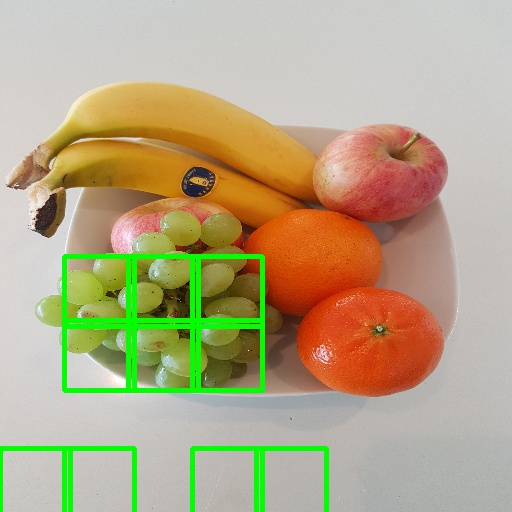
\includegraphics[scale=0.4]{fruitFromPhoneRR_13Classes}
      \caption{Image after sliding window - 13 classes}
      \label{fig:fruitRR13}
\end{figure}

\begin{figure}[h]
	\centering
    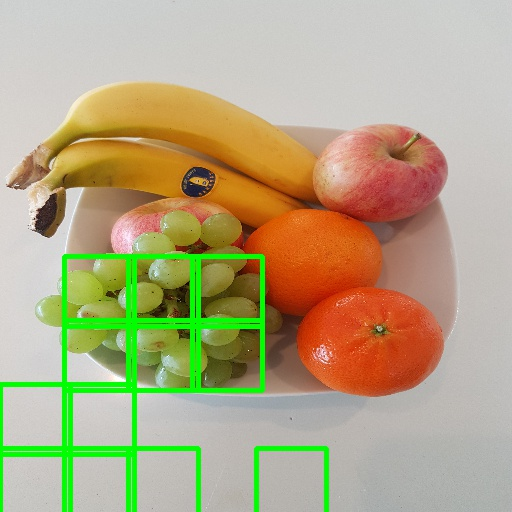
\includegraphics[scale=0.4]{fruitFromPhoneRR_108Classes}
      \caption{Image after sliding window - 108 classes}
      \label{fig:fruitRR108}
\end{figure}

\begin{table}[]
\centering
\caption{Results of recursive refinement segment classifications using two models}
\label{RR_result_table}
\begin{tabular}{|l|l|l|}
\hline
\textbf{Fruitbowl Segment} & \textbf{13 class model}                                                                                                                                       & \textbf{108 class model}                                                                                                                                   \\ \hline
False Positive 1                 & \begin{tabular}[c]{@{}l@{}}grape 0.31476045\\ apple 0.25866747\\ orange 0.11228518\\ apple pie 0.10234257\\ chocolate cake 0.09062083\end{tabular}   & \begin{tabular}[c]{@{}l@{}}grape 0.31820437\\ panna cotta 0.091400646\\ macarons 0.08560496\\ roll 0.08188102\\ apple 0.03981942\end{tabular}     \\ \hline
False Positive 2                 & \begin{tabular}[c]{@{}l@{}}grape 0.29391274\\ apple 0.2371384\\ orange 0.16196558\\ chocolate cake 0.10039616\\ apple pie 0.096121624\end{tabular}   & \begin{tabular}[c]{@{}l@{}}panna cotta 0.21783036\\ grape 0.105718106\\ apple 0.087030284\\ macarons 0.07753955\\ orange 0.037592527\end{tabular} \\ \hline
False Positive 3                 & \begin{tabular}[c]{@{}l@{}}grape 0.22402291\\ chocolate cake 0.16412543\\ apple 0.14523567\\ orange 0.12525927\\ apple pie 0.099948086\end{tabular}  & \begin{tabular}[c]{@{}l@{}}grape 0.2835378\\ panna cotta 0.088551655\\ macarons 0.06166248\\ orange 0.041896477\\ roll 0.040348493\end{tabular}   \\ \hline
False Positive 4                 & \begin{tabular}[c]{@{}l@{}}apple 0.37422368\\ grape 0.28592423\\ orange 0.10230055\\ chocolate cake 0.085367255\\ apple pie 0.053731006\end{tabular} & \begin{tabular}[c]{@{}l@{}}grape 0.20476209\\ macarons 0.17529227\\ panna cotta 0.16139281\\ roll 0.04359601\\ orange 0.036991216\end{tabular}    \\ \hline
False Positive 5                 & N/A                                                                                                                                                  & \begin{tabular}[c]{@{}l@{}}grape 0.22574392\\ macarons 0.14840269\\ panna cotta 0.08670294\\ roll 0.08650105\\ orange 0.046900786\end{tabular}    \\ \hline
False Positive 6                 & N/A                                                                                                                                                  & \begin{tabular}[c]{@{}l@{}}grape 0.31369162\\ panna cotta 0.11833602\\ macarons 0.09010604\\ apple 0.057512555\\ roll 0.047116004\end{tabular}    \\ \hline
\end{tabular}
\end{table}

\tocless\subsection{Analysis}
\tocless\subsubsection{Comparing the two models}
As we can see evidence of in Table \ref{RR_result_table}, along with Figure \ref{fig:fruitRR13} and Figure \ref{fig:fruitRR108}, the model trained on 13 classes predicted only four false positives while the larger model predicted 6.
This is most likely due to the larger model not being able to separate grapes as well as the smaller model.
It is worth mentioning that the grape class has the lowest number of training images of all the other classes.

\tocless\subsubsection{Analysing Probabilities}
The probabilities of predictions for grapes in these false positive classifications are all low, in both models.
In contrast, some of the correctly classified segments were run through the model and the results all had probabilities in the high nineties.
When these background segments are run through the model, some prediction has to be made and none of these false predictions have a probability of over 0.4.
The average probability of these segments being grapes is in fact 0.257 (rounded to three decimal places).
A counter measure to this problem could be to disregard any predictions with a probability under a certain threshold, perhaps 0.4.



\section{Scaling Down Images}
\label{scale}
\begin{figure}
    \includegraphics[scale=0.5]{fruitbowl2}
    \caption{Alternative Bowl of fruit}
    \label{fig:newFruit}
\end{figure}

\subsection*{Overview}
In our three previous sliding window oriented experiments, we had only used a
single image. In order to see whether this image had biases unknown
to us, I decided to use another fruit bowl image. This image was selected as
fruit took up a larger portion of the image as seen in Figure \ref{fig:newFruit}

\subsection*{Results}
\subsubsection*{Grid}
\subsubsection*{Row}
\subsubsection*{Column}

\subsection*{Analysis}


\section{Effect of Colour}
\label{colour}
\tocless\subsection{Objective}
As seen in the last experiment, it is possible that colour plays a significant part in the overall classification of some food types, along with shape and texture. Due to this, what would happen if colour was removed from the image? The three images, Figure \ref{fig:bananaPreRes}, Figure \ref{fig:apple_piePreRes} and Figure \ref{fig:pizzaPreRes}, were all converted to greyscale to test this and the resulting images can be seen in Figure \ref{fig:bananaGrey}, Figure \ref{fig:applePieGrey} and Figure \ref{fig:pizzaGrey}. Each of these images were ran through the model before and after converting to greyscale and the results were recorded.

\begin{figure}[h]
	\centering
    \includegraphics[scale=0.05]{banana_grey}
    \caption{Banana Image Greyscale}
    \label{fig:bananaGrey}
\end{figure}

\begin{figure}[h]
	\centering
    \includegraphics[scale=0.25]{pie_grey}
    \caption{Apple Pie Image Greyscale}
    \label{fig:applePieGrey}
\end{figure}

\begin{figure}[h]
	\centering
    \includegraphics[scale=0.05]{pizza_grey}
    \caption{Pizza Image Greyscale}
    \label{fig:pizzaGrey}
\end{figure}

\tocless\subsection{Results}
The results for this experiment can be seen in Table \ref{colour}.
The 'Top 1' notation in the table suggests that the food was predicted as the number one prediction. The decimal value is the probability of that food type being the correct classification.

\begin{table}[]
\centering
\caption{Effect of Colour}
\label{colour}
\begin{tabular}{|l|l|l|}
\hline
\textbf{Food Image} & \textbf{Pre-Scaled Image} & \textbf{Greyscale}      \\ \hline
Banana     & Top 1 : 0.9971   & Top 1 : 0.9986 \\ \hline
Apple Pie  & Top 1 : 0.7986   & Top 1 : 0.3462   \\ \hline
Pizza      & Top 1 : 0.9753   & Top 2 : 0.1299 \\ \hline
\end{tabular}
\end{table}

\tocless\subsection{Analysis}
\tocless\subsubsection{Colour}
In regard to the images of the banana (Figure \ref{fig:bananaPreRes} and Figure \ref{fig:bananaGrey}), there is very little difference in classification. They were both classified to a Top 1 accuracy and their probabilities differing by only 0.0015 with the grey scale image being of a higher probability. This would indicate that colour is not an important factor for classifying bananas and the coloured image may even have noise. This can be seen in Table \ref{colour}.

The apple pie images (Figure \ref{fig:apple_piePreRes} and Figure \ref{fig:applePieGrey}) were also both classified correctly but with a large gap in the likelihood of that classification being correct. As per Table \ref{colour}, the coloured image had a probability of 0.7986 as opposed to one of 0.3462. This would indicate that while colour is important, there is enough unique data from the rest of the image to result in correct classification.

Finally, the pizza images (Figure \ref{fig:pizzaPreRes} and Figure \ref{fig:pizzaGrey}) were the most contrasting in their results. While the original image was classified to Top 1 accuracy with a likelihood of 0.9753, the coloured image was classified to Top 2 accuracy with a probability of 0.1299. From this we can deduce that colour is vital for the classification of pizza.

Since this experiment only compared three images, we cannot say for sure if this analysis is biased or not.

\tocless\subsubsection{Colour vs Scale}
In the last experiment, it was seen that the pizza and banana images (Figure \ref{fig:pizzaPreRes} and Figure \ref{fig:bananaPreRes}) were not really affected by image quality. While this seems to be true, the image of apple pie, Figure \ref{fig:apple_piePreRes}, was greatly influenced by only being classified to a Top 5 accuracy when down scaled.

For the greyscale images, bananas were not effected greatly and neither was an apple pie but a pizza was greatly influenced.

From this, it can be said that the prominent unique features for each of these food types are different. The banana (Figure \ref{fig:bananaPreRes}) may have focus on shape and texture, the pie (Figure \ref{fig:apple_piePreRes}) on image quality and some influence of colour while the pizza (Figure \ref{fig:pizzaPreRes}) may have a focus on shape, texture and colour.



\section{Visualising Images Through the Network}
\label{visualise}
\tocless\subsection{Overview}
\tocless\subsection{Network Architecture}
\tocless\subsection{Dataset}
\tocless\subsection{API's}
\tocless\subsection{Script}
\tocless\subsection{Results}
\tocless\subsection{Empirical Analysis}



\chapter{Prototype Application}
\label{prototype}
In order to demonstrate practical use of the models trained in Chapter 4, a prototype application was developed.
This application was developed for a smartphone running on the Android operating system in the Java programming language.
A backend service was created to receive an image from the smartphone
application, process the image using the CNN previously developed and return a
response to the application in the form of a prediction.

\section{Requirements}
Lightweight requirements elicitation was carried out for this FYP.
Since prototyping itself is an elicitation technique \parencite{reqs}, the requirements for this prototype application did not need to be extensive.
Myself and my supervisor acted as stakeholders for this project as users of the system.
Two methods of elicitation were used for this project sourced from \parencite{reqs}.
These elicitation techniques were data gathering from an existing system and brain storming.

In a previous FYP, a mobile application was developed for nutritional assessment.
The use of this application provided the opportunity to elicit requirements based on data gathered from this system. Brainstorming also took place between the stakeholders for requirements elicitation.

\tocless\subsection{Functional Requirements}
The functional requirements for this application can be seen in Table \ref{requirements}.

\begin{longtable}{|p{.75cm}|p{3.5cm}|p{6cm}|p{2.5cm}|}
\hline
\textbf{ID} & \textbf{Title}                                              & \textbf{Description}                                                                                    & Dependencies                                   \\ \hline
R1          & Open application from Android phone                         & A user can open the application from a list of applications on their Android phone.                     &                                                \\ \hline
R2          & Choose to take a photo                                      & A user can choose to take a photo of a food item.                                                       & R1                                             \\ \hline
R3          & Take a photo                                                & A user can take a photo using the application.                                                          & R1, R2                                         \\ \hline
R4          & Confirm the photo                                           & A user can confirm the photo captured is sufficient.                                                    & R1, R2, R3                                     \\ \hline
R5          & Retry photo capture                                         & A user can retry the capturing of an image.                                                             & R1, R2, R3                                     \\ \hline
R6          & Send the image to be classified                             & A user can send an image of a food item to be classified.                                               & R1, R2, R3, R4                                 \\ \hline
R7          & Cancel sending an image                                     & A user can cancel sending an image.                                                                    & R1, R2, R3, R4                                 \\ \hline
R8          & Classify the food image                                     & The system can classify an image as a food type.                                                        & R1, R2, R3, R4, R6                             \\ \hline
R9          & View the food image classification                          & A user can view the classification made of the image.                                                   & R1, R2, R3, R4, R6, R8                         \\ \hline
R10         & View the calorie information of the food classification     & A user can view the calorie information of the classified food type.                                    & R1, R2, R3, R4, R6, R8                         \\ \hline
R11         & Change the food classification data                         & A user can change the food classification data if they are unhappy with it.                             & R1, R2, R3, R4, R6, R8, R9                     \\ \hline
R12         & Change the calorie information                              & A user can change the calorie information if they are unhappy with it.                                  & R1, R2, R3, R4, R6, R8, 10                     \\ \hline
R13         & Submit the food classification and calorie data for logging & A user can submit the data calculated such as classification data and calorie information to be logged. & R1, R2, R3, R4, R6, R8, R9, R10                \\ \hline
R14         & Save food log data                                          & The system can save information for logging.                                                            & R1, R2, R3, R4, R6, R8, R9, R10, R13           \\ \hline
R15         & Choose to classify an image from the phone's storage        & A user can choose to select an image from the phone's storage to be classified.                         & R1                                             \\ \hline
R16         & Choose an image from phone's storage                        & A user can choose an image from the phone's storage to classify.                                        & R1, R14                                        \\ \hline
R17         & Choose to view food logs                                    & A user can choose to view the food logs saved on their device.                                          & R1                                             \\ \hline
R18         & View food logs by day                                       & A user can view the food logs saved on the device by day.                                               & R1, R2, R3, R4, R6, R8, R9, R10, R13, R17      \\ \hline
R19         & View food logs by week                                      & A user can view the food logs saved on the device by week.                                              & R1, R2, R3, R4, R6, R8, R9, R10, R13, R17      \\ \hline
R20         & View food logs by month                                     & A user can view the food logs saved on the device by month.                                             & R1, R2, R3, R4, R6, R8, R9, R10, R13, R17      \\ \hline
R21         & View total calories recorded per day                        & A user can view the total calorie count recorded per day.                                               & R1, R2, R3, R4, R6, R8, R9, R10, R13, R17      \\ \hline
R22         & View total calories recorded per week                       & A user can view the total calorie count recorded per week.                                              & R1, R2, R3, R4, R6, R8, R9, R10, R13, R17      \\ \hline
R23         & View total calories recorded per month                      & A user can view the total calorie count recorded per month.                                             & R1, R2, R3, R4, R6, R8, R9, R10, R13, R17      \\ \hline
R24         & Delete a food log                                           & A user can delete an individual food log.                                                               & R1, R2, R3, R4, R6, R8, R9, R10, R13, R17, R18 \\ \hline
\caption{Functional Requirements}
\label{requirements}
\end{longtable}

\tocless\subsection{Non-Functional Requirements}
The nature of a prototype application does not call for non-functional requirements.
Despite this, some non-functional requirements were kept in mind during the development of this application such as:
\begin{itemize}
	\item{Performance - for example, how long it takes for an image to be classified.}
	\item{Extensibility - is it easy to extend the functionality of the system.}
	\item{Maintainability - how easy it is to maintain the system.}
	\item{Usability - how easy it is to use the system.}
\end{itemize}

\clearpage

\section{Design}
The design process for this prototype application consisted of user interface design, android application system design and the activity of choosing resources for a backend host.

\subsection*{User Interface}
The user interface mock ups were created using \parencite{fluid}.
The aim of this design was to provide a simple, easy to use interface so that a user could use the application with minimal effort.
The main benefit of using computer vision for this type of application is to
reduce the effort of the user or dietician keeping track of food intake.
Therefore, this application had to be very quick and easy to use.
The application is called NutriLog.

Three main activities were needed for this application.
The first activity, as seen in Figure \ref{fig:page1}, would consist of options to either take an image of food or to view the food logs of the user.
If the user decides to take an image of food, they will be brought to the second activity which can be seen in Figure \ref{fig:page2}.
The user is required to take a picture before reaching the activity in Figure \ref{fig:page2}.
Once the user presses the send button the image is classified and the content of the activity changes to display the classification and calorie count as in Figure \ref{fig:page3}.
Alternatively, the user can cancel the process and return to the first activity.
The user would then submit the food classification for logging and automatically return to the first activity.
The final activity is displayed when a user views their food logs.
This activity has the ability to view a list of the food logs taken by the user by day, week or month.
The calorie count of the selected time frame is to be displayed on this activity also.

\begin{figure}[h] 
  \label{ fig7} 
  \begin{minipage}[b]{0.5\linewidth}
    \centering
    \includegraphics[width=.75\linewidth]{Mockup1} 
    \caption{Landing Activity} 
  \label{fig:page1}
    \vspace{4ex}
  \end{minipage}%%
  \begin{minipage}[b]{0.5\linewidth}
    \centering
    \includegraphics[width=.75\linewidth]{Mockup2} 
    \caption{Image Submission Activity} 
  \label{fig:page2}
    \vspace{4ex}
  \end{minipage} 
  \begin{minipage}[b]{0.5\linewidth}
    \centering
    \includegraphics[width=.75\linewidth]{Mockup3} 
    \caption{Classification Activity} 
    \label{fig:page3}
    \vspace{4ex}
  \end{minipage}%% 
  \begin{minipage}[b]{0.5\linewidth}
    \centering
    \includegraphics[width=.75\linewidth]{Mockup4} 
    \caption{Food Logs Activity} 
    \label{fig:page4}
    \vspace{4ex}
  \end{minipage} 
\end{figure}
\afterpage{\clearpage}

\subsection*{System Architecture}

\begin{figure}[h]
    \centering
    \includegraphics[scale=0.15]{packageDiagram}
    \caption{Package Diagram}
    \label{fig:packageDiagram}
\end{figure}

\subsubsection*{Architectural Patterns}
The Model-View-Presenter (MVP) architectural pattern was adapted for this application \parencite{mvp}.
This pattern is very similar to the Model-View-Controller (MVC) architecture which is quite popular in the software development industry.
The main difference between MVC and MVP is that whereas in MVC the controller is responsible for which view is used, in MPV the presenter is called through the view.
This is due to the architecture of Android applications in general, where the view takes primary control.
In the view classes, there should be no logic whatsoever in an MVP architecture and all logic should be called in the presenters.
There is also a one to one dependency between views and presenters.

As illustrated in Figure \ref{fig:packageDiagram}, the views in the application
have a dependency only on their corresponding presenter.
The presenters contain the business logic of the  application and have a dependency on all other packages.
The packages of backgroundProcesses, calorieEstimation and storage have a dependancy on the presenters package for callback purposes and also database creation in Android requires context of the activity information.

\subsubsection*{Marchitecture}
In Figure \ref{fig:market}, a marchitecture diagram can be seen.
This diagram represents the architecture of the system.
NutriLog is an Android application that send an image to an AWS (Amazon Web Services) instance using the API OkHttp. The AWS instance is running a Python FLASK application that classifies the image using a TensorFlow model and sends a response back to NutriLog. The Nutritionix API is used to collect nutritional information of this classification.

\begin{figure}[h]
    \centering
    \includegraphics[scale=0.15]{market}
    \caption{Marchitecture Diagram}
    \label{fig:market}
\end{figure}

The technologies used for this appliction were used for the following reasons:

\textbf{AWS}
\linebreak
Past experience was a large factor when it came to choosing a cloud provider to host the backend instance for this prototype application.
AWS instances are very easy to set up once the process has been carried out a few times and this was a contributing factror to why AWS was chosen.
AWS also has a free tier which provides all the necessary server space to host the backend service for this application.

\textbf{OkHttp}
\linebreak
OkHttp seemed to be popular for Android applications as seen on websites such as Stack Overflow.
OkHttp also has extensive documentation and is a very simple API to import into Android.
The learning curve for OkHttp is quite small and it doesn't require much code to carry out a simple task like sending a HTTP POST request to a backend instance.

\textbf{FLASK}
\linebreak
Python FLASK was used for the backend service in this FYP due to past experience and its simplicity.

\textbf{TensorFlow}
\linebreak
TensorFlow was chosen as the library to create neural networks for this FYP mostly because of its reputation.
TensorFlow has been used by many researches in the computer vision industry.
TensirFlow also has extensive documentation and a wide array or resources and tutorials.

\textbf{Nutritionix}
\linebreak
Nutrionix was the best nutrional information API that was also free to use and this is why it was chosen.

\section{Implementation}
Outlined below are some coding fragments categorised under: Design Patterns, Asynchronous Tasks, Presenters, Views and Interesting Coding Fragments.

\tocless\subsection{Design Patterns}
Various design patterns were used in the implementation of this application such as the Factory, the Builder and the Singleton which are outlined below.

The Factory design pattern was used to retrieve a DAO (Data Access Object) as seen in Figure \ref{lst:daoFactory}.
This was used so that if at a future time the storage type of the application is to be changed, the developer would only have to change one instance of the codebase and return a new implementation of the DAO interface in the method getDAO().
\begin{figure}[h]
\caption{DAO Factory Class}
\label{lst:daoFactory}
\begin{lstlisting}[style=Java]
public class DAOFactory {

    public DAO getDAO(Context context){
        return SqlLiteDAO.getInstance(context);
    }
}
\end{lstlisting}
\end{figure}

A Host builder was used to create a Host object.
This builder is a static inner class in the Host class file as documented in Figure \ref{lst:hostBuilder}
\begin{figure}[h]
\caption{HostBuilder Class}
\label{lst:hostBuilder}
\begin{lstlisting}[style=Java]
public static class HostBuilder {
    private final String ipv4;
    private String dns;
    private int port;
    private String route;

    public HostBuilder(String ipv4) {
        this.ipv4 = ipv4;
    }

    public HostBuilder withDns(String dns) {
        this.dns = dns;
        return this;
    }

    public HostBuilder withPort(int port) {
        this.port = port;
        return this;
    }

    public HostBuilder withRoute(String route) {
        this.route = route;
        return this;
    }

    public Host build() {
        return new Host(this);
    }

}
\end{lstlisting}
\end{figure}

A Singleton instance of the DAO implementation was used in this application.
This was mainly due to the best practice of keeping database access objects as singleton instances.
This class can be seen in Figure \ref{lst:singletonDao}.

\begin{figure}[h]
\caption{Singleton DAO Object}
\label{lst:singletonDao}
\begin{lstlisting}[style=Java]
public static DAO getInstance(Context context) {
    if(instance == null) {
        instance = new SqlLiteDAO(context);
    }
    return instance;
}
\end{lstlisting}
\end{figure}

\tocless\subsection{Asynchronous Tasks}
Asynchronous Tasks in Android are used to run tasks in the background or are sometimes used to simply distribute processes off the main thread.
The AsyncTask class must be extended on creation of the background processes.
An AsyncTask was used to send the food image to the backend host as in Figure \ref{lst:rrCode}.
\begin{figure}[h]
\caption{UploadImage Class}
\label{lst:rrCode}
\begin{lstlisting}[style=Java]
@Override
protected String doInBackground(Void... params) {
    String result = "";
    OkHttpClient client = new OkHttpClient();
    String imageToSend = image;
    RequestBody requestBody = new MultipartBody.Builder()
            .setType(MultipartBody.FORM)
            .addFormDataPart("image", imageToSend)
            .build();

    Request request = new Request.Builder().url(host.getUrl())
            .post(requestBody).build();

    Response response = null;
    try {
        response = client.newCall(request).execute();
        result = response.body().string();
        response.body().close();
    } catch (IOException e) {
        e.printStackTrace();
    }

    return result;
}
\end{lstlisting}
\end{figure}

\tocless\subsection{Presenters}
In the MPV architecture as described earlier, the presenter for each activity contains all the logic for that view.
The presenter in Figure \ref{lst:pres} was tasked with creating intents to new activities (views).
\begin{figure}[h]
\caption{MainPresenter Class}
\label{lst:pres}
\begin{lstlisting}[style=Java]
public class MainPresenter {

    private Intent intent;
    private Context context;

    public MainPresenter(Context context) {
        this.context=context;
    }

    public void takePhoto() {
        intent = new Intent(context, CaptureImageActivity.class);
        context.startActivity(intent);
    }

    public void userLogs() {
        intent = new Intent(context, FoodLogsActivity.class);
        context.startActivity(intent);
    }

}
\end{lstlisting}
\end{figure}

\tocless\subsection{Views}
In the MPV architecture that this application uses, the views are responsible for interacting directly with the user interface.
The view for the MainActivity in Figure \ref{lst:mainView} responds to button clicks and calls to its presenter to carry out the logic of the required task.
\begin{figure}[h]
\caption{MainActivity Class}
\label{lst:mainView}
\begin{lstlisting}[style=Java]
public class MainActivity extends AppCompatActivity {

    private MainPresenter mainPresenter;

    @Override
    protected void onCreate(Bundle savedInstanceState) {
        super.onCreate(savedInstanceState);
        setContentView(R.layout.activity_main);

        mainPresenter = new MainPresenter(this);
    }

    public void onClickTakePhoto(View view) {
        mainPresenter.takePhoto();
    }

    public void onClickUserLogs(View view) {
        mainPresenter.userLogs();
    }
}
\end{lstlisting}
\end{figure}

\tocless\subsection{Storage}
SQLite was used for storing data in this application and the class that handled creation, input and output to this database implemented the DAO interface.
An interface for storage devices was created so that each implementation would have the ability to add food logs, retrieve food logs, delete food logs and remove the data store completely.
This is documented in Figure \ref{lst:daoInterface}.
\begin{figure}[h]
\caption{DAO Interface}
\label{lst:daoInterface}
\begin{lstlisting}[style=Java]
public interface DAO {
    void addFoodLog(FoodLog foodLog);
    List<FoodLog> getLogsByDay(Date date);
    List<FoodLog> getLogsByWeek(Date date);
    List<FoodLog> getLogsByMonth(Date date);
    void deleteFoodLogs(List<FoodLog> foodLogs);
    void deleteDb();
}
\end{lstlisting}
\end{figure}

The method in Figure \ref{lst:getLogs} was used to execute a query and return a List of FoodLog objects.
\begin{figure}[h]
\caption{Get Food Logs Per Date}
\label{lst:getLogs}
\begin{lstlisting}[style=Java]
@Override
private List<FoodLog> selectQuery(String query) {
        foodLogs = new ArrayList<>();
        Cursor resultSet = database.rawQuery(query, null);
        while(resultSet.moveToNext()) {
            try {
                foodLogs.add(new FoodLogImpl
                .FoodLogBuilder(resultSet.getString(1))
                .withId(resultSet.getInt(0))
                .withCalories(resultSet.getDouble(2))
                .withTimestamp(dateFormat
                    .parse(resultSet.getString(3)))
                .build());
            } catch (ParseException e) {
                e.printStackTrace();
            }
        }
    return foodLogs;
}
\end{lstlisting}
\end{figure}

\tocless\subsection{Interesting Coding Fragments}
Some interesting coding fragments are outlined below which merit inclusion in this report.

The method in Figure \ref{lst:encodeBitmap} was used to encode the image taken on the phone to a string.
This was used to send the image to the backend with minimal latency.
The bitmap size was also reduced as in line 8 to decrease response time also.
\begin{figure}[h]
\caption{Encode Bitmap to base64 String}
\label{lst:encodeBitmap}
\begin{lstlisting}[style=Java]
public String toBase64() {
    BitmapFactory.Options options = new BitmapFactory.Options();
    options.inSampleSize = 8;

    Bitmap imageBitmap = BitmapFactory.decodeFile(image.getAbsolutePath(), options);

    //resize image for faster upload to server
    Bitmap.createScaledBitmap(imageBitmap, 300, 400, false);
    
    ByteArrayOutputStream byteArrayOutputStream = new ByteArrayOutputStream();
    imageBitmap.compress(Bitmap.CompressFormat.PNG, 100, byteArrayOutputStream);
    byte[] byteArray = byteArrayOutputStream.toByteArray();

    return Base64.encodeToString(byteArray, Base64.DEFAULT);
}
\end{lstlisting}
\end{figure}

A map of strings to runnables was used to query the database for food logs as documented in Figure \ref{lst:map}.
This was used as the select query for the database had to dynamically change depending on how the food logs were being viewed, by day, week, or month.
\begin{figure}[h]
\caption{Map of Runnables}
\label{lst:map}
\begin{lstlisting}[style=Java]
listViewOptions = new HashMap<>();
listViewOptions.put("Day", () -> getLogsByDay());
listViewOptions.put("Week",() -> getLogsByWeek());
listViewOptions.put("Month", () -> getLogsByMonth());
\end{lstlisting}
\end{figure}

\tocless\subsection{User Interface}
User interface implementation as in Figures \ref{fig:gallery}, \ref{fig:ui2}, \ref{fig:ui3}, \ref{fig:ui5}, \ref{fig:ui8}, \ref{fig:ui6}, \ref{fig:ui7} and \ref{fig:delete}.

\begin{figure}
  \label{uiDesign1} 
  \begin{minipage}[b]{0.5\linewidth}
    \centering
    \includegraphics[width=.75\linewidth]{gallery} 
    \caption{Landing Activity} 
  \label{fig:gallery}
    \vspace{4ex}
  \end{minipage}%%
  \begin{minipage}[b]{0.5\linewidth}
    \centering
    \includegraphics[width=.75\linewidth]{ui2} 
    \caption{Image Capture Activity} 
  \label{fig:ui2}
    \vspace{4ex}
  \end{minipage} 
  \begin{minipage}[b]{0.5\linewidth}
    \centering
    \includegraphics[width=.75\linewidth]{ui3} 
    \caption{Image Send Activity} 
    \label{fig:ui3}
    \vspace{4ex}
  \end{minipage}%% 
  \begin{minipage}[b]{0.5\linewidth}
    \centering
    \includegraphics[width=.75\linewidth]{ui5} 
    \caption{Image Submit Activity} 
    \label{fig:ui5}
    \vspace{4ex}
  \end{minipage} 
\end{figure}

\begin{figure}
  \label{uiDesign2} 
  \begin{minipage}[b]{0.5\linewidth}
    \centering
    \includegraphics[width=.75\linewidth]{ui8} 
    \caption{FoodLog Month Activity} 
    \label{fig:ui8}
    \vspace{4ex}
  \end{minipage}
  \begin{minipage}[b]{0.5\linewidth}
    \centering
    \includegraphics[width=.75\linewidth]{ui6} 
    \caption{FoodLog Day Activity} 
  \label{fig:ui6}
    \vspace{4ex}
  \end{minipage} 
  \begin{minipage}[b]{0.5\linewidth}
    \centering
    \includegraphics[width=.75\linewidth]{ui7} 
    \caption{FoodLog Week Activity} 
    \label{fig:ui7}
    \vspace{4ex}
  \end{minipage}%% 
  \begin{minipage}[b]{0.5\linewidth}
    \centering
    \includegraphics[width=.75\linewidth]{delete} 
    \caption{Food Log Deletion} 
  \label{fig:delete}
    \vspace{4ex} 
    \end{minipage}%% 
\end{figure}
\clearpage

\tocless\subsection{Technologies}

\tocless\subsubsection{GitHub}
GitHub was used as the version control backup system for this project.
Commit history can be seen in Figure \ref{fig:git}

\begin{figure}[h]
    \includegraphics[scale=0.5]{git}
    \caption{GitHub Contributions to Master}
    \label{fig:git}
\end{figure}

\tocless\subsubsection{JSON}
JSON (JavaScript Object Notation) is a text format used to store data \parencite{json}.
It is both easy for machines to parse and for humans to read and write.
It is a data-interchange format as it is language independent.
JSON data structures are built on key pairs values and are normally parsed into arrays, lists or vectors.

\tocless\subsubsection{OkHttp}
OkHttp is a HTTP client created specifically for Java and Android applications \parencite{okhttp}.
It is a very efficient HTTP client with inbuilt defense against troublesome networks (recovers from common problems silently).
Some of the efficiency components are as follows:
\begin{itemize}
    \item{HTTP/2 support.}
    \item{Reduced request latency due to connection pooling.}
    \item{Caching of responses.}
\end{itemize}

\tocless\subsubsection{Nutritionix API}
The Nutritionix API is an API used to collect nutritional information \parencite{nutritionix}.
This project used this API to collect calorie information on a food item.
The free 'Hacker' account can support up to 10 active users.

\tocless\subsection{Software Quality Attributes}
Two main software quality attributes were focused on during the implementation of this prototype application. These were extensibility and maintainability.

Extensibility defines how easy it is to extend the functionality of the system.
There were certain places where the system developed is highly extensible.
A factory class was used to get the data access object that was used to store information in the application.
This factory class has a factory method that returns a DAO object which is an interface.
If the developer of the system needs to create an alternative way to store data in the application, they can create an object that implements the DAO interface and replace one line of code in the factory class.
A factory class was also used to create a Host object with the same rationale.

Maintainability defines how easy it is to maintain a system.
The system is maintainable for many reasons.
These reasons include low coupling, high cohesion and readability.






\section{Testing}
JUnit tests were used to test this prototype application.
JUnit is a unit testing framework.
Mockito is a framework for JUnit that was also utilised.
Mockito makes mocks of objects for testing.
This is very useful to test database instances as you can mock an SQLite Database object.

\tocless\subsection{Unit Tests}
Evidence of some unit tests written for this prototype application can be seen in Figures \ref{lst:test1}, \ref{lst:test2} and \ref{lst:test3}.
Figure \ref{fig:unitTests} also displays the automated tests that were run from Android Studio.

\begin{figure}[h]
    \includegraphics[scale=0.5]{UnitTests}
    \caption{Automated Unit Tests}
    \label{fig:unitTests}
\end{figure}

\begin{figure}[h]
\caption{Test to ensure FoodLog object stores information correctly}
\label{lst:test1}
\begin{lstlisting}[style=Java]
@Before
public void setUp() {
    foodLog = new FoodLogImpl(0, "banana", 59.03, new Date());
}

@Test
public void shouldAssertCorrectValues() {
    assert food.equals(foodLog.getFood());
    assert calories == foodLog.getCalories();
    assert timestamp.equals(foodLog.getTimestamp());
    assert id == foodLog.getId();
}
\end{lstlisting}
\end{figure}

\begin{figure}[h]
\caption{Test to ensure Host object stores information correctly}
\label{lst:test2}
\begin{lstlisting}[style=Java]
@Before
    public void setUp() {
        host = new Host.HostBuilder("52.214.205.157")
                .withDns("ec2-52-214-205-157.eu-west-1.compute.amazonaws.com")
                .withPort(5000)
                .withRoute("/classifyImage/")
                .build();
    }

@Test
public void shouldAssertCorrectValues() {
    assert this.ip.equals(host.getIpv4());
    assert this.dns.equals(host.getDns());
    assert this.port == host.getPort();
    assert this.route.equals(host.getRoute());
    assert this.urlString.equals(host.getUrl());
}
\end{lstlisting}
\end{figure}

\begin{figure}[h]
\caption{Test to ensure DAO object stores and removes data correctly}
\label{lst:test3}
\begin{lstlisting}[style=Java]
@Before
public void setup() {
    dao = mock(SqlLiteDAO.class);
    date = new Date();
    foodLog = new FoodLogImpl(0, "test", 0.0, date);
}

@Test
public void shouldGetListOfFoodLogs() {
    foodLogs = dao.getLogsByDay(date);
    foodLogs = dao.getLogsByWeek(date);
    foodLogs = dao.getLogsByMonth(date);
}

@Test
public void shouldInsertFoodLogToDao() {
    dao.addFoodLog(foodLog);
    setTestLog();
    assert foodLogs.contains(testLog);
}

@Test
public void shouldDeleteFoodLog() {
    List<FoodLog> foodLogs = new ArrayList<>();
    foodLogs.add(testLog);
    dao.deleteFoodLogs(foodLogs);
    setTestLog();
    assert testLog.equals(null);
}

private void setTestLog() {
    foodLogs = dao.getLogsByDay(date);
    foodLogs.forEach(f -> {
        if(f.getFood().equals("test")) {
            testLog = f;
        }
    });
}
\end{lstlisting}
\end{figure}

\clearpage

\section{Backend}
\tocless\subsection{Python Flask}

\tocless\subsection{Implementation}
Figures \ref{lst:backendCode} and \ref{lst:labelBackend} document the code used to implement the backend service.

\begin{figure}[h]
\caption{Backend service code}
\label{lst:backendCode}
\begin{lstlisting}[style=Python]
import base64
import label_image
import time

app = Flask(_name_)

#add a route for the flask app and what HTTP methods are allowed
@app.route('/classifyImage/', methods=['POST'])
def classify():
    #decode image and save it
    imgdata = base64.b64decode(request.form.get('image'))
    filename = 'images/' + str(time.strftime("%Y%m%d-%H%M%S")) + '.jpg'
    with open(filename, 'wb') as f:
        f.write(imgdata)

    #classify the image
    results = label_image.runModel(filename)
    predictions = results[0]

    #retrun a String of the results
    result_String = ""
    for i in predictions :
        result_String += str(i) + ","
    return result_String

#runs the app on port 5000
if _name_ == '_main_':
    app.run(host='0.0.0.0', threaded=True)
\end{lstlisting}
\end{figure}

\begin{figure}[h]
\caption{Method called from 'label\_image.py' - adapted from \parencite{retrainInception}}
\label{lst:labelBackend}
\begin{lstlisting}[style=Python]
def runModel(file_name):
  #hardcoded values of image size and model path
  model_file = \
    "models/output_graph13.pb"
  label_file = "labels/output_labels13.txt"
  input_height = 299
  input_width = 299
  input_mean = 128
  input_std = 128
  input_layer = "Mul"
  output_layer = "final_result"

  #load the graph using load_graph() provided be Google
  graph = load_graph(model_file)
  #read in tensor
  t = read_tensor_from_image_file(file_name,
                                  input_height=input_height,
                                  input_width=input_width,
                                  input_mean=input_mean,
                                  input_std=input_std)

  input_name = "import/" + input_layer
  output_name = "import/" + output_layer
  input_operation = graph.get_operation_by_name(input_name)
  output_operation = graph.get_operation_by_name(output_name)

  #run the tensor through the graph
  with tf.Session(graph=graph) as sess:
    results = sess.run(output_operation.outputs[0],
                      {input_operation.outputs[0]: t})
  results = np.squeeze(results)

  #get the top 5 results
  top_k = results.argsort()[-5:][::-1]
  labels = load_labels(label_file)

  setIndex = False

  #return results
  top5_results = [None] * 5
  index = 0
  for i in top_k:
    top5_results[index] = labels[i]
    index += 1

  final_results = [top5_results, results]
  return final_results
\end{lstlisting}
\end{figure}

\tocless\subsection{Deployment}
In order to deploy the Flask application to an AWS EC2 instance the following steps had to be followed:

\begin{itemize}
    \item{Upload the output\_graph.pb file (TensorFlow model), the output\_labels.txt file and the source code to the server using SFTP.}
    \item{SSH into the server.}
    \item{Create a folder called 'images' in the home directory to store uploads images.}
    \item{Place model and label files into folders called 'models' and 'labels' respectively.}
    \item{Ensure TensorFlow, Python and Flask are installed on the server.}
    \item{Ensure no processes are running on port 5000 using the command 'lsof -i :5000'.}
    \item{Use the command 'screen'.}
    \item{Run the server.py code using the command 'python server.py'.}
    \item{Use the commands CTRL+A and CRTL+D to exit screen.}
\end{itemize}

\tocless\subsubsection{AWS Architecture}
The application interfaces with an Amazon Web Services (AWS) server called an EC2 instance.
To keep the application secure AWS was used to provide a secure architecture.
A Virtual Private Cloud (VPC) was created to host the instances.
In a production environment a load balancer could be used to evenly distribute traffic across a fleet of backend instances but for the purposes of this prototype application, a single instance as in Figure \ref{fig:aws} could be used.
In Figure \ref{fig:aws} the instance is located inside a subnet which is in turn located in a VPC.
The purpose of a VPC is to have a virtual network dedicated to a users individual account. 
\begin{figure}[h]
    \centering
    \includegraphics{aws}
    \caption{AWS Network Diagram}
    \label{fig:aws}
\end{figure}

Security groups were utilised to restrict the type of traffic that would be allowed to reach the instance, so that the instance would only receive HTTP requests at port 5000 and receive SSH connections at port 22 as per Figure \ref{fig:awsSecGroup}.
\begin{figure}[h]
    \centering
    \includegraphics{secGroups}
    \caption{AWS Security Group}
    \label{fig:awsSecGroup}
\end{figure}

% \begin{itemize}
%     \item{Upload the output_graph.pb file (Tensorflow model), the output_labels.txt file and the source code to the server using SFTP}
%     \item{SSH into the server}
%     \item{Create a folder called 'images' in the home directory to store uploads images}
%     \item{Place model and label files into folders called 'models' and 'labels' respectively}
%     \item{Ensure Tensorflow, NOHUP (Ignores the hangup signal in Linux) Python and Flask are installed on the server}
%     \item{Ensure no processes are running on port 5000 using the command 'lsof -i :5000'}
%     \item{Run the server.py code using the command 'nohup python server.py &'}
% \end{itemize}
\chapter{Discussion and Conclusion}
\section{Summary}
The purpose of this final year project was to explore the use of deep learning for nutritional assessment.
This exploration was carried firstly by conducting a comprehensive literature review of research already undertaken in the area of food image recognition and also some research into the methods used for object detection with CNNs.
Once this survey of literature was completed, a method from these papers was selected to be replicated.
The work done by \parencite{yanaiFood} yielded promising results in retraining models using transfer learning and because of this, their work was to be replicated.

Some deviations were made from \parencite{yanaiFood} in regard to the dataset used.
The Food-101 dataset was used for this FYP, in conjunction with some additional classes from ImageNet \parencite{imagenet}.
In contrast, \parencite{yanaiFood} used the UECFOOD100 dataset \parencite{uecFood}.
The change in dataset was used due to the availability of a larger dataset in Food-101 which has 1,000 images per class.

The Food-101+ dataset was created by adding seven additional classes to the Food-101 dataset.
This Food-101+ dataset was used to train a model with the final Top-1 accuracy of 66.6\% and a Top-5 accuracy of  85.96\%.
This model was created by retraining the final layer of the Inception-V3 \parencite{rethinkingInception} model using transfer learning and TensorFlow.
A subset of the Food-101+ dataset was also trained using 13 classes in the same way.
This model achieved a Top-1 accuracy of 92.6\% and a Top-5 accuracy of 100\%.

Once the models were trained, they were analysed under various topics such as
dealing with composite images using a sliding window approach, the effect of colour on classification of food types and the effect of image quality on the classification of food types.

After the above empirical studies had been carried out, a lightweight prototype application was created to demonstrate the use of the TensorFlow model for food image classification.
This prototype application was created for a smart phone running on Android.
This application is called NutriLog.
NutriLog is able to send an image of food (acquired either from the camera or gallery of the users phone) to a server to be analysed.
The server that the image is sent to is running a Python Flask application that runs the image through a TensorFlow model and returns a prediction to NutriLog.
NutriLog then collects nutritional information on the prediction using the Nutritionix API and logs information for user metrics.
The user can then view their daily, weekly or monthly calorie intake.
NutriLog could be very useful for those who wish to keep track of their calorie intake.

\section{Reflections}
The purpose of this section is to give a reflection upon the technologies I have used throughout this project.
I will outline my feelings on each of these technologies in the following sections.

\tocless\subsection{TensorFlow}
There are many alternative machine learning libraries used for the development of CNNs such as Caffe, Gluon and MXNet.
I used TensorFlow due to Google's reputation and prevalence on the Internet.
While TensorFlow has a large learning curve, I believe this is due to the complexity of CNNs and machine learning in general rather than the library.
I used Python in conjunction with TensorFlow in this project.

The online support for TensorFlow is superb.
From resources such as Stack Overflow to Google's forums for questions relating to the topic.
While I don't have experience with the other libraries, I would definitely recommend TensorFlow to beginners in machine learning as the documentation and support is outstanding.

\tocless\subsection{Python}
Python is a very simple and generic programming language supporting the paradigms of object oriented, functional, imperative and procedural.
I enjoyed working with the language for the most part.
It seems like the language is written to make things as easy as possible for the developer with many helpful in-built functions.

Python is a dynamically typed language meaning that type checking is carried out at runtime as opposed to statically typed when it is carried out at compile time.
Personally, I prefer statically typed languages.
This could be partly due to my experience in Java (which is statically typed) by I find when dealing with code that has been written by another developer, something as simple as knowing the types of function parameters is taken for granted.

\tocless\subsection{Flask}
Flask is a web framework that integrates with Python.
I cannot stress how nice it is to use.
It has a very small learning curve and its makes prototyping web services very easy.

\tocless\subsection{AWS}
I have had previous experience with Amazon Web Services on a summer internship and while working on college projects.
Due to this past experience, there was no hesitation in choosing a cloud provider for my prototype application.
A simple EC2 instance is very easy to setup using AWS.

\tocless\subsection{Android Studio}
Android Studio is the IDE used for the development of Android applications.
It is made by JetBrains who also developed the IDE InteliJ so there are many similarities there.
For the most part it is like InteliJ which is very nice to use for Java development.
The UI design in Android Studio is also very good as most of the UI development can be done in a drag and drop fashion which is very helpful for prototyping.

\tocless\subsection{Java}
I have been using Java for four years and it is a very nice language to use especially with the introduction of streams and other functional paradigms addition.

\tocless\subsection{Latex}
I used Latex for the report for this FYP due to the suggestion from my supervisor.
Overall, I find it a very good resource to use.
The fact that you focus more on content than presentation is very helpful for such a large report and the use of version control is very beneficial.
The positioning of images and tables is sometimes a bit frustrating, but I found Latex the most useful when I wanted to move sections around in the report and for references.

\section{Future Work}
While retraining the Inception-V3 model yielded promising results for food image classification there are some problems associated.
The model trained, does not deal well with composite image and while a sliding window could be used to classify different portions of the image, it is not a viable method as it is very time intensive.
Another issue is that there is a clear correlation between the number of classes and the accuracy of the model.
This is clearly seen in the 108 class model yielding a Top-1 accuracy of 66.6\% while the 13 class model yielded a Top-1 accuracy of 92.6\%.
Possible solutions to these issues are outlined below.

\tocless\subsection{Resolving Issues with Composite Images}
The model trained for this project relies on the one-shot approach where an image is passed straight to the model preferable containing only one food item.
A possible solution to this problem is to segment the image before using the classifier.
There has been extensive research into the segmentation of food images carried out, but it was out of scope for this FYP.
Colour and texture are the most common features to segment food images by.
If it was possible to separate each food item in a food image and feed each of these individual items through the classifier then the problem of composite image would be resolved.

Another option would be to take an object detection approach to food image classification.
In Chapter 2 there was a survey of literature carried about
using CNNs for object detection as in \parencite{maskRcnn}.
If the objects (food items) could be detected in this way and then passed through the classifier then dealing with composite images would not be such a challenge.

While both of these methods are promising approaches to solving this issue, the object detection seems to be a good approach. This is due to the success of \parencite{maskRcnn}, although the method has not been used for food images before.

\tocless\subsection{Resolving Issues with Class Size}
As stated above, the accuracy of Inception-V3 model declines the more classes are in the training set.
In order to solve this problem changes to the architecture of the model or
changes to the dataset may have to be introduced.
There are many CNN model architectures that could be viable options for food image recognition.
\parencite{nutrinet} created a model architecture aimed specifically towards food image recognition called Nutrinet and experiments on this architecture could be carried out.
The dataset used for training could also be extended with more images per class to increase the accuracy.


\nocite{*}

\printbibliography

\begin{appendices}
\chapter{Segmentation}
\section{Image Segmentation}
\subsection*{Fully Convolutional Neural Networks for Semantic Segmentation}
There has been a very interesting paper from UC Berkeley focused on using Full Convolutional
Networks for semantic segmentation \parencite{fcn}. Fully Convolutional Networks
(FCN)
do not have any fully connected layers. They are replaced with more filtering
layers. Nvidia Digits have a semantic segmentation implementation based off the
work of this paper.

They took this approach because "feedforward computation and backpropogation are
much more efficient when computer layer-by-layer over an entire image instead of
independently patch-by-patch" \parencite{fcn}. This was also because they
were focused on object detection. Normal classifiers do not work very well when
they are to classify more than one subject in an image and image segmentation
was a way to solve this.

There are a set of steps you can follow to turn a CNN into a FCN for semantic
segmentation as follows ie. change to a convolutional layer from a fully
connected one:
\begin{itemize}
    \item{The size of the filters must be set to the size of the input layers.}
    \item{For every neuron in the fully connected layer, have a filter.}
\end{itemize}

\begin{table}[]
\centering
\caption{FCN Resulys \parencite{fcn}}
\label{fcn}
\begin{tabular}{ll}
                        & FCN  \\
VOC11 mean IU           & 62.7 \\
VOC12 mean IU           & 62.2 \\
PASCAL VOC10 pixel acc. & 67.0 \\
PASCAL VOC10 mean acc.  & 50.7 \\
PASCAL VOC10 mean IU    & 37.8 \\
PASCAL VOC10 f.w. IU    & 52.5
\end{tabular}
\end{table}

\subsection*{Segmentation}
\subsubsection*{Graph Based Segmentation}
Graph cut segmentation has been used extensively  in image segmentation. OpenCV
has an implementation of a graph cut algorithm called grabcut which has been
used to segment food on occasion \textcite{graphCut}. 

According to \textcite{graphCut}, "Graph cut based method is well-known to be
efficient, robust, and capable of finding the best contour of objects in n
image, suggesting it to be a good method for separating food portions in a food
image for calorie measurement". Along with the graph cut segmentation algorithm,
this research team also used color and texture segmentation. Gabor filters were
used to measure texture features \textcite{graphCut}. When color and texture
segmentation was applied, the method came into difficulty with mixed foods but
by applying graph cut segmentation, clearer object boundaries were shown.

In conclusion, the accuracy of the classification increased when using graph
based segmentation rather than color and texture as seen in \ref{graphCT}.

\begin{table}[]
	\centering
	\caption{Results}
	\label{graphCT}
	\begin{tabular}{llll}
		                  & Single Food Portion & Non-mixed Food & Mixed Food
						  \\
						  Color and Texture & 92.21               & N/A
						  & N/A           \\
						  Graph Based       & 95 (3\% increase)   & 5\% increase
						  & 15\% increase
	\end{tabular}
\end{table}

\subsubsection*{Local Variation Framework}
Another paper was published in which the research team attempted to create a
food calorie extimation system \textcite{foodImageAnalysis}. This system would
compromise of three steps, image segmentation, image classification and weight
estimation. For the segmentation module, a local variation approach to
segmentation was performed. Local variation is by which intensity differences
between neighbouring pixels is measured. This is a type of graph based
segmentation.

The team also carried out some segmentation refinement when the segmentation
algorithm had been performed. This consisted of removed small segments (defined
as less than 50 pixels) and trying to prevent over and under segmentation. After
classification was performed on each segment, segments with low confidence
values were removed \textcite{foodImageAnalysis}.

\subsubsection*{Conclusion}
Both of the above papers of \textcite{graphCut} and \textcite{foodImageAnalysis}
used a graph based segmentation. The first paper used a more generic
implementation while the second used a local variation framework. Both methods
provided successful results in the image segmentation process.


\includepdf{tex/poster}

% \begin{figure}
%     \includegraphics[width=150mm,scale=0.5]{DAP}
%     \caption{Detection Average Precision \parencite{donahue}}
%     \label{fig:dap}
% \end{figure}

% \begin{figure}
%     \includegraphics[width=150mm,scale=0.5]{MAP}
%     \caption{Mean Average Precision \parencite{donahue}}
%     \label{fig:MAP}
% \end{figure}

% \begin{figure}
%     \includegraphics[width=150mm,scale=0.5]{DFP}
%     \caption{Distribution of top-ranked false positives
%     \parencite{donahue}}
%     \label{fig:DFP}
% \end{figure}

% \begin{figure}
%     \includegraphics[width=150mm,scale=0.5]{SMP}
%     \caption{Segmentation Mean Accuracy \parencite{donahue}}
%     \label{fig:SMP}
% \end{figure}

% \begin{figure}
%     \includegraphics[width=150mm,scale=0.5]{PCATSA}
%     \caption{Per-category segmentation accuracy \parencite{donahue}}
%     \label{fig:PCATSA}
% \end{figure}

% \begin{figure}
%     \includegraphics[width=150mm,scale=0.5]{PCLASSSA}
%     \caption{Per-class segmentation accuracy \parencite{donahue}}
%     \label{fig:PCLASSA}
% \end{figure}

% \begin{table}[]
%     \centering
%     \caption{Project Plan}
%     \label{pp}
%     \begin{tabular}{ll}
%         Task/Deliverable                     & Deadline \\
%         Interim Report                       & 21/12/17 \\
%         Select method and paper to replicate & 10/01/18 \\
%         Iteration 1                          & ???      \\
%         Iteration 2                          & ???      \\
%         Iteration 3                          & ???      \\
%         Draft Final Report                   & 08/03/18 \\
%         FYP Product                          & 10/04/18 \\
%         FYP Report                           & 17/04/18
%     \end{tabular}
% \end{table}


\chapter{Poster}
% \section{Demo Day Poster}
% A poster was created for the demo day for this FYP.
\includepdf{tex/poster}

\end{appendices}

\end{document}   
